\documentclass[a4paper]{book}
\usepackage{a4wide}
\usepackage{makeidx}
\usepackage{fancyhdr}
\usepackage{graphicx}
\usepackage{multicol}
\usepackage{float}
\usepackage{textcomp}
\usepackage{alltt}
\usepackage{doxygen}
\makeindex
\setcounter{tocdepth}{1}
\renewcommand{\footrulewidth}{0.4pt}
\begin{document}
\begin{titlepage}
\vspace*{7cm}
\begin{center}
{\Large Lib\-TIM Reference Manual}\\
\vspace*{1cm}
{\large Generated by Doxygen 1.4.4}\\
\vspace*{0.5cm}
{\small Fri Sep 8 12:19:22 2006}\\
\end{center}
\end{titlepage}
\clearemptydoublepage
\pagenumbering{roman}
\tableofcontents
\clearemptydoublepage
\pagenumbering{arabic}
\chapter{Lib\-TIM Module Index}
\section{Lib\-TIM Modules}
Here is a list of all modules:\begin{CompactList}
\item \contentsline{section}{Morphological Operators}{\pageref{group__Morpho}}{}
\begin{CompactList}
\item \contentsline{section}{Component-Tree Based Algorithms}{\pageref{group__ccTree}}{}
\item \contentsline{section}{Connected Components Labelling}{\pageref{group__ccLabelling}}{}
\item \contentsline{section}{Basis Functions}{\pageref{group__basisFunctions}}{}
\item \contentsline{section}{Regional Extrema Extraction}{\pageref{group__extremaExtraction}}{}
\item \contentsline{section}{Geodesic Reconstruction}{\pageref{group__reconstruction}}{}
\item \contentsline{section}{Connected Operators}{\pageref{group__connectedOperators}}{}
\item \contentsline{section}{Interval Operators}{\pageref{group__interval}}{}
\item \contentsline{section}{Region Growing Algorithms}{\pageref{group__regionGrowing}}{}
\item \contentsline{section}{Constrained Watershed Algorithms}{\pageref{group__constrainedWatershed}}{}
\item \contentsline{section}{Watershed-based Algorithms}{\pageref{group__watershed}}{}
\end{CompactList}
\item \contentsline{section}{Image Processing Basis Functions}{\pageref{group__ImageProcessing}}{}
\begin{CompactList}
\item \contentsline{section}{Distance Transform}{\pageref{group__DistanceTransform}}{}
\item \contentsline{section}{K-Means}{\pageref{group__kMeans}}{}
\item \contentsline{section}{Misc Functions}{\pageref{group__misc}}{}
\item \contentsline{section}{Tarjan's Union Find Algorithms}{\pageref{group__Tarjan}}{}
\item \contentsline{section}{Template Matching Based Algorithms}{\pageref{group__templateMatching}}{}
\item \contentsline{section}{Thresholding Functions}{\pageref{group__thresholding}}{}
\end{CompactList}
\item \contentsline{section}{Data Structures}{\pageref{group__DataStructures}}{}
\begin{CompactList}
\item \contentsline{section}{Flat Structuring Elements}{\pageref{group__FlatSE}}{}
\item \contentsline{section}{Histogram}{\pageref{group__Histogram}}{}
\item \contentsline{section}{Image}{\pageref{group__Image}}{}
\item \contentsline{section}{Non-flat structuring elements}{\pageref{group__NonFlatSE}}{}
\item \contentsline{section}{Point}{\pageref{group__Point}}{}
\end{CompactList}
\end{CompactList}

\chapter{Lib\-TIM Directory Hierarchy}
\section{Lib\-TIM Directories}
This directory hierarchy is sorted roughly, but not completely, alphabetically:\begin{CompactList}
\item \contentsline{section}{Algorithms}{\pageref{dir_000000}}{}
\item \contentsline{section}{Common}{\pageref{dir_000001}}{}
\end{CompactList}

\chapter{Lib\-TIM Namespace Index}
\section{Lib\-TIM Namespace List}
Here is a list of all namespaces with brief descriptions:\begin{CompactList}
\item\contentsline{section}{{\bf Lib\-TIM} (Lib\-TIM library )}{\pageref{namespaceLibTIM}}{}
\item\contentsline{section}{{\bf std} }{\pageref{namespacestd}}{}
\end{CompactList}

\chapter{Lib\-TIM Hierarchical Index}
\section{Lib\-TIM Class Hierarchy}
This inheritance list is sorted roughly, but not completely, alphabetically:\begin{CompactList}
\item \contentsline{section}{Lib\-TIM::Flat\-SE}{\pageref{classLibTIM_1_1FlatSE}}{}
\begin{CompactList}
\item \contentsline{section}{Lib\-TIM::Non\-Flat\-SE$<$ T $>$}{\pageref{classLibTIM_1_1NonFlatSE}}{}
\end{CompactList}
\item \contentsline{section}{Lib\-TIM::Histogram$<$ T $>$}{\pageref{classLibTIM_1_1Histogram}}{}
\item \contentsline{section}{Lib\-TIM::Image$<$ T $>$}{\pageref{classLibTIM_1_1Image}}{}
\item \contentsline{section}{Lib\-TIM::Image\-Iterator$<$ TImage, T $>$}{\pageref{classLibTIM_1_1ImageIterator}}{}
\begin{CompactList}
\item \contentsline{section}{Lib\-TIM::Image\-Iterator\-XYZ$<$ TImage, T $>$}{\pageref{classLibTIM_1_1ImageIteratorXYZ}}{}
\end{CompactList}
\item \contentsline{section}{Lib\-TIM::Image\-Regions\-Infos$<$ T, T2 $>$}{\pageref{classLibTIM_1_1ImageRegionsInfos}}{}
\item \contentsline{section}{Lib\-TIM::Node}{\pageref{structLibTIM_1_1Node}}{}
\item \contentsline{section}{Lib\-TIM::Ordered\-Queue$<$ T $>$}{\pageref{classLibTIM_1_1OrderedQueue}}{}
\item \contentsline{section}{Lib\-TIM::Ordered\-Queue\-Double$<$ T $>$}{\pageref{classLibTIM_1_1OrderedQueueDouble}}{}
\item \contentsline{section}{Lib\-TIM::Point$<$ T $>$}{\pageref{classLibTIM_1_1Point}}{}
\item \contentsline{section}{Lib\-TIM::Queue$<$ T $>$}{\pageref{classLibTIM_1_1Queue}}{}
\item \contentsline{section}{Random}{\pageref{classRandom}}{}
\item \contentsline{section}{Lib\-TIM::Region}{\pageref{structLibTIM_1_1Region}}{}
\item \contentsline{section}{Lib\-TIM::Table$<$ T, N $>$}{\pageref{structLibTIM_1_1Table}}{}
\end{CompactList}

\chapter{Lib\-TIM Class Index}
\section{Lib\-TIM Class List}
Here are the classes, structs, unions and interfaces with brief descriptions:\begin{CompactList}
\item\contentsline{section}{{\bf Lib\-TIM::Flat\-SE} (Container base class for flat structuring elements (or binary masks) )}{\pageref{classLibTIM_1_1FlatSE}}{}
\item\contentsline{section}{{\bf Lib\-TIM::Histogram$<$ T $>$} (Container for histograms )}{\pageref{classLibTIM_1_1Histogram}}{}
\item\contentsline{section}{{\bf Lib\-TIM::Image$<$ T $>$} (Container base for images of generic type T in {\bf Lib\-TIM}{\rm (p.\,\pageref{namespaceLibTIM})} )}{\pageref{classLibTIM_1_1Image}}{}
\item\contentsline{section}{{\bf Lib\-TIM::Image\-Iterator$<$ TImage, T $>$} }{\pageref{classLibTIM_1_1ImageIterator}}{}
\item\contentsline{section}{{\bf Lib\-TIM::Image\-Iterator\-XYZ$<$ TImage, T $>$} }{\pageref{classLibTIM_1_1ImageIteratorXYZ}}{}
\item\contentsline{section}{{\bf Lib\-TIM::Image\-Regions\-Infos$<$ T, T2 $>$} }{\pageref{classLibTIM_1_1ImageRegionsInfos}}{}
\item\contentsline{section}{{\bf Lib\-TIM::Node} }{\pageref{structLibTIM_1_1Node}}{}
\item\contentsline{section}{{\bf Lib\-TIM::Non\-Flat\-SE$<$ T $>$} (Non-flat structuring elements (or ponderated masks) )}{\pageref{classLibTIM_1_1NonFlatSE}}{}
\item\contentsline{section}{{\bf Lib\-TIM::Ordered\-Queue$<$ T $>$} (Ordered {\bf Queue}{\rm (p.\,\pageref{classLibTIM_1_1Queue})} )}{\pageref{classLibTIM_1_1OrderedQueue}}{}
\item\contentsline{section}{{\bf Lib\-TIM::Ordered\-Queue\-Double$<$ T $>$} (Ordered {\bf Queue}{\rm (p.\,\pageref{classLibTIM_1_1Queue})} with double priority )}{\pageref{classLibTIM_1_1OrderedQueueDouble}}{}
\item\contentsline{section}{{\bf Lib\-TIM::Point$<$ T $>$} ({\bf Point}{\rm (p.\,\pageref{classLibTIM_1_1Point})} Structure )}{\pageref{classLibTIM_1_1Point}}{}
\item\contentsline{section}{{\bf Lib\-TIM::Queue$<$ T $>$} }{\pageref{classLibTIM_1_1Queue}}{}
\item\contentsline{section}{{\bf Random} }{\pageref{classRandom}}{}
\item\contentsline{section}{{\bf Lib\-TIM::Region} }{\pageref{structLibTIM_1_1Region}}{}
\item\contentsline{section}{{\bf Lib\-TIM::Table$<$ T, N $>$} }{\pageref{structLibTIM_1_1Table}}{}
\end{CompactList}

\chapter{Lib\-TIM File Index}
\section{Lib\-TIM File List}
Here is a list of all files with brief descriptions:\begin{CompactList}
\item\contentsline{section}{Algorithms/{\bf Adaptative\-SE.h} }{\pageref{AdaptativeSE_8h}}{}
\item\contentsline{section}{Algorithms/{\bf Adaptative\-SE.hxx} }{\pageref{AdaptativeSE_8hxx}}{}
\item\contentsline{section}{Algorithms/{\bf Component\-Tree.h} }{\pageref{ComponentTree_8h}}{}
\item\contentsline{section}{Algorithms/{\bf Component\-Tree.hxx} }{\pageref{ComponentTree_8hxx}}{}
\item\contentsline{section}{Algorithms/{\bf Connected\-Components.h} }{\pageref{ConnectedComponents_8h}}{}
\item\contentsline{section}{Algorithms/{\bf Connected\-Components.hxx} }{\pageref{ConnectedComponents_8hxx}}{}
\item\contentsline{section}{Algorithms/{\bf Distance\-Transform.h} }{\pageref{DistanceTransform_8h}}{}
\item\contentsline{section}{Algorithms/{\bf Distance\-Transform.hxx} }{\pageref{DistanceTransform_8hxx}}{}
\item\contentsline{section}{Algorithms/{\bf KMeans.h} }{\pageref{KMeans_8h}}{}
\item\contentsline{section}{Algorithms/{\bf KMeans.hxx} }{\pageref{KMeans_8hxx}}{}
\item\contentsline{section}{Algorithms/{\bf Misc.h} }{\pageref{Misc_8h}}{}
\item\contentsline{section}{Algorithms/{\bf Misc.hxx} }{\pageref{Misc_8hxx}}{}
\item\contentsline{section}{Algorithms/{\bf Morphology.h} }{\pageref{Morphology_8h}}{}
\item\contentsline{section}{Algorithms/{\bf Morphology.hxx} }{\pageref{Morphology_8hxx}}{}
\item\contentsline{section}{Algorithms/{\bf random-singleton.cpp} }{\pageref{random-singleton_8cpp}}{}
\item\contentsline{section}{Algorithms/{\bf random-singleton.h} }{\pageref{random-singleton_8h}}{}
\item\contentsline{section}{Algorithms/{\bf Region\-Growing.h} }{\pageref{RegionGrowing_8h}}{}
\item\contentsline{section}{Algorithms/{\bf Region\-Growing.hxx} }{\pageref{RegionGrowing_8hxx}}{}
\item\contentsline{section}{Algorithms/{\bf Tarjan.h} }{\pageref{Tarjan_8h}}{}
\item\contentsline{section}{Algorithms/{\bf Tarjan.hxx} }{\pageref{Tarjan_8hxx}}{}
\item\contentsline{section}{Algorithms/{\bf Template\-Matching.h} }{\pageref{TemplateMatching_8h}}{}
\item\contentsline{section}{Algorithms/{\bf Template\-Matching.hxx} }{\pageref{TemplateMatching_8hxx}}{}
\item\contentsline{section}{Algorithms/{\bf Thresholding.h} }{\pageref{Thresholding_8h}}{}
\item\contentsline{section}{Algorithms/{\bf Thresholding.hxx} }{\pageref{Thresholding_8hxx}}{}
\item\contentsline{section}{Algorithms/{\bf Viscous\-Watershed.h} }{\pageref{ViscousWatershed_8h}}{}
\item\contentsline{section}{Algorithms/{\bf Viscous\-Watershed.hxx} }{\pageref{ViscousWatershed_8hxx}}{}
\item\contentsline{section}{Algorithms/{\bf Watershed.h} }{\pageref{Watershed_8h}}{}
\item\contentsline{section}{Algorithms/{\bf Watershed.hxx} }{\pageref{Watershed_8hxx}}{}
\item\contentsline{section}{Common/{\bf Flat\-SE.h} }{\pageref{FlatSE_8h}}{}
\item\contentsline{section}{Common/{\bf Flat\-SE.hxx} }{\pageref{FlatSE_8hxx}}{}
\item\contentsline{section}{Common/{\bf Histogram.h} }{\pageref{Histogram_8h}}{}
\item\contentsline{section}{Common/{\bf Histogram.hxx} }{\pageref{Histogram_8hxx}}{}
\item\contentsline{section}{Common/{\bf Image.h} }{\pageref{Image_8h}}{}
\item\contentsline{section}{Common/{\bf Image.hxx} }{\pageref{Image_8hxx}}{}
\item\contentsline{section}{Common/{\bf Image\-IO.hxx} }{\pageref{ImageIO_8hxx}}{}
\item\contentsline{section}{Common/{\bf Image\-Iterators.h} }{\pageref{ImageIterators_8h}}{}
\item\contentsline{section}{Common/{\bf Non\-Flat\-SE.h} }{\pageref{NonFlatSE_8h}}{}
\item\contentsline{section}{Common/{\bf Non\-Flat\-SE.hxx} }{\pageref{NonFlatSE_8hxx}}{}
\item\contentsline{section}{Common/{\bf Ordered\-Queue.h} }{\pageref{OrderedQueue_8h}}{}
\item\contentsline{section}{Common/{\bf Point.h} }{\pageref{Point_8h}}{}
\item\contentsline{section}{Common/{\bf Types.h} }{\pageref{Types_8h}}{}
\end{CompactList}

\chapter{Lib\-TIM Module Documentation}
\section{Component-Tree Based Algorithms}
\label{group__ccTree}\index{Component-Tree Based Algorithms@{Component-Tree Based Algorithms}}
\subsection*{Functions}
\begin{CompactItemize}
\item 
void {\bf Lib\-TIM::filter\-Area} ({\bf t\-Node} $\ast$root, int area)
\item 
void {\bf Lib\-TIM::print\-Tree} ({\bf t\-Node} $\ast$tree)
\item 
void {\bf Lib\-TIM::make\_\-father} ({\bf t\-Node} $\ast$$\ast$$\ast$index, int label1, int label2, int h1, int h2)
\item 
{\bf t\-Node} $\ast$ {\bf Lib\-TIM::init\_\-tree} (void)
\item 
Image$<$ {\bf U8} $>$ {\bf Lib\-TIM::reconstruct\-Image} ({\bf t\-Node} $\ast$tree, const {\bf TSize} $\ast$size)
\begin{CompactList}\small\item\em Reconstruct image from tree. \item\end{CompactList}\item 
template$<$class T$>$ {\bf t\-Node} $\ast$ {\bf Lib\-TIM::compute\-Component\-Tree} (Image$<$ T $>$ \&im, Flat\-SE \&se)
\item 
void {\bf Lib\-TIM::father} ({\bf t\-Node} $\ast$tree, {\bf t\-Node} $\ast$child)
\item 
{\bf t\-Node} $\ast$ {\bf Lib\-TIM::init\_\-tree} (int h, int n)
\item 
template$<$class T$>$ {\bf t\-Node} $\ast$ {\bf Lib\-TIM::compute\-Component\-Tree\-Bens\-Method} (Image$<$ T $>$ \&im, Flat\-SE \&se)
\item 
int {\bf Lib\-TIM::compute\-Area} ({\bf t\-Node} $\ast$tree)
\item 
template$<$class T$>$ int {\bf Lib\-TIM::flood} (Image$<$ T $>$ \&im, std::map$<$ int, std::queue$<$ int $>$ $>$ \&oq, int h, int h\-Min, vector$<$ int $>$ \&STATUS, vector$<$ int $>$ \&number\_\-nodes, vector$<$ bool $>$ \&node\_\-at\_\-level, Flat\-SE \&se, std::map$<$ T, std::map$<$ {\bf TLabel}, struct Node $\ast$ $>$ $>$ \&index)
\item 
template$<$class T$>$ int {\bf Lib\-TIM::flood2} (Image$<$ T $>$ \&im, std::map$<$ int, std::queue$<$ int $>$ $>$ \&oq, int h, int h\-Min, vector$<$ int $>$ \&STATUS, vector$<$ int $>$ \&number\_\-nodes, vector$<$ bool $>$ \&node\_\-at\_\-level, Flat\-SE \&se, std::map$<$ T, std::map$<$ {\bf TLabel}, struct Node $\ast$ $>$ $>$ \&index)
\begin{CompactList}\small\item\em New method to deal with neighbors. \item\end{CompactList}\item 
template$<$class T$>$ {\bf t\-Node} $\ast$ {\bf Lib\-TIM::compute\-Component\-Tree2V1} (Image$<$ T $>$ \&im, Flat\-SE \&se)
\begin{CompactList}\small\item\em Following Salembier recursive implementation... \item\end{CompactList}\item 
template$<$class T$>$ {\bf t\-Node} $\ast$ {\bf Lib\-TIM::compute\-Component\-Tree2} (Image$<$ T $>$ \&im, Flat\-SE \&se)
\begin{CompactList}\small\item\em Following Salembier recursive implementation... \item\end{CompactList}\end{CompactItemize}


\subsection{Function Documentation}
\index{ccTree@{cc\-Tree}!computeArea@{computeArea}}
\index{computeArea@{computeArea}!ccTree@{cc\-Tree}}
\subsubsection{\setlength{\rightskip}{0pt plus 5cm}int Lib\-TIM::compute\-Area ({\bf t\-Node} $\ast$ {\em tree})}\label{group__ccTree_ga9}


\index{ccTree@{cc\-Tree}!computeComponentTree@{computeComponentTree}}
\index{computeComponentTree@{computeComponentTree}!ccTree@{cc\-Tree}}
\subsubsection{\setlength{\rightskip}{0pt plus 5cm}template$<$class T$>$ {\bf t\-Node}$\ast$ Lib\-TIM::compute\-Component\-Tree (Image$<$ T $>$ \& {\em im}, Flat\-SE \& {\em se})}\label{group__ccTree_ga5}


Build the component tree of image im Return a structure containing the image max-tree For now: trivial algorithm \index{ccTree@{cc\-Tree}!computeComponentTree2@{computeComponentTree2}}
\index{computeComponentTree2@{computeComponentTree2}!ccTree@{cc\-Tree}}
\subsubsection{\setlength{\rightskip}{0pt plus 5cm}template$<$class T$>$ {\bf t\-Node}$\ast$ Lib\-TIM::compute\-Component\-Tree2 (Image$<$ T $>$ \& {\em im}, Flat\-SE \& {\em se})}\label{group__ccTree_ga13}


Following Salembier recursive implementation... 

\index{ccTree@{cc\-Tree}!computeComponentTree2V1@{computeComponentTree2V1}}
\index{computeComponentTree2V1@{computeComponentTree2V1}!ccTree@{cc\-Tree}}
\subsubsection{\setlength{\rightskip}{0pt plus 5cm}template$<$class T$>$ {\bf t\-Node}$\ast$ Lib\-TIM::compute\-Component\-Tree2V1 (Image$<$ T $>$ \& {\em im}, Flat\-SE \& {\em se})}\label{group__ccTree_ga12}


Following Salembier recursive implementation... 

\index{ccTree@{cc\-Tree}!computeComponentTreeBensMethod@{computeComponentTreeBensMethod}}
\index{computeComponentTreeBensMethod@{computeComponentTreeBensMethod}!ccTree@{cc\-Tree}}
\subsubsection{\setlength{\rightskip}{0pt plus 5cm}template$<$class T$>$ {\bf t\-Node}$\ast$ Lib\-TIM::compute\-Component\-Tree\-Bens\-Method (Image$<$ T $>$ \& {\em im}, Flat\-SE \& {\em se})}\label{group__ccTree_ga8}


\index{ccTree@{cc\-Tree}!father@{father}}
\index{father@{father}!ccTree@{cc\-Tree}}
\subsubsection{\setlength{\rightskip}{0pt plus 5cm}void Lib\-TIM::father ({\bf t\-Node} $\ast$ {\em tree}, {\bf t\-Node} $\ast$ {\em child})}\label{group__ccTree_ga6}


\index{ccTree@{cc\-Tree}!filterArea@{filterArea}}
\index{filterArea@{filterArea}!ccTree@{cc\-Tree}}
\subsubsection{\setlength{\rightskip}{0pt plus 5cm}void Lib\-TIM::filter\-Area ({\bf t\-Node} $\ast$ {\em root}, int {\em area})}\label{group__ccTree_ga0}


\index{ccTree@{cc\-Tree}!flood@{flood}}
\index{flood@{flood}!ccTree@{cc\-Tree}}
\subsubsection{\setlength{\rightskip}{0pt plus 5cm}template$<$class T$>$ int Lib\-TIM::flood (Image$<$ T $>$ \& {\em im}, std::map$<$ int, std::queue$<$ int $>$ $>$ \& {\em oq}, int {\em h}, int {\em h\-Min}, vector$<$ int $>$ \& {\em STATUS}, vector$<$ int $>$ \& {\em number\_\-nodes}, vector$<$ bool $>$ \& {\em node\_\-at\_\-level}, Flat\-SE \& {\em se}, std::map$<$ T, std::map$<$ {\bf TLabel}, struct Node $\ast$ $>$ $>$ \& {\em index})}\label{group__ccTree_ga10}


\index{ccTree@{cc\-Tree}!flood2@{flood2}}
\index{flood2@{flood2}!ccTree@{cc\-Tree}}
\subsubsection{\setlength{\rightskip}{0pt plus 5cm}template$<$class T$>$ int Lib\-TIM::flood2 (Image$<$ T $>$ \& {\em im}, std::map$<$ int, std::queue$<$ int $>$ $>$ \& {\em oq}, int {\em h}, int {\em h\-Min}, vector$<$ int $>$ \& {\em STATUS}, vector$<$ int $>$ \& {\em number\_\-nodes}, vector$<$ bool $>$ \& {\em node\_\-at\_\-level}, Flat\-SE \& {\em se}, std::map$<$ T, std::map$<$ {\bf TLabel}, struct Node $\ast$ $>$ $>$ \& {\em index})}\label{group__ccTree_ga11}


New method to deal with neighbors. 

\index{ccTree@{cc\-Tree}!init_tree@{init\_\-tree}}
\index{init_tree@{init\_\-tree}!ccTree@{cc\-Tree}}
\subsubsection{\setlength{\rightskip}{0pt plus 5cm}{\bf t\-Node}$\ast$ Lib\-TIM::init\_\-tree (int {\em h}, int {\em n})}\label{group__ccTree_ga7}


\index{ccTree@{cc\-Tree}!init_tree@{init\_\-tree}}
\index{init_tree@{init\_\-tree}!ccTree@{cc\-Tree}}
\subsubsection{\setlength{\rightskip}{0pt plus 5cm}{\bf t\-Node}$\ast$ Lib\-TIM::init\_\-tree (void)}\label{group__ccTree_ga3}


\index{ccTree@{cc\-Tree}!make_father@{make\_\-father}}
\index{make_father@{make\_\-father}!ccTree@{cc\-Tree}}
\subsubsection{\setlength{\rightskip}{0pt plus 5cm}void Lib\-TIM::make\_\-father ({\bf t\-Node} $\ast$$\ast$$\ast$ {\em index}, int {\em label1}, int {\em label2}, int {\em h1}, int {\em h2})}\label{group__ccTree_ga2}


\index{ccTree@{cc\-Tree}!printTree@{printTree}}
\index{printTree@{printTree}!ccTree@{cc\-Tree}}
\subsubsection{\setlength{\rightskip}{0pt plus 5cm}void Lib\-TIM::print\-Tree ({\bf t\-Node} $\ast$ {\em tree})}\label{group__ccTree_ga1}


\index{ccTree@{cc\-Tree}!reconstructImage@{reconstructImage}}
\index{reconstructImage@{reconstructImage}!ccTree@{cc\-Tree}}
\subsubsection{\setlength{\rightskip}{0pt plus 5cm}Image$<${\bf U8}$>$ Lib\-TIM::reconstruct\-Image ({\bf t\-Node} $\ast$ {\em tree}, const {\bf TSize} $\ast$ {\em size})\hspace{0.3cm}{\tt  [inline]}}\label{group__ccTree_ga4}


Reconstruct image from tree. 


\section{Connected Components Labelling}
\label{group__ccLabelling}\index{Connected Components Labelling@{Connected Components Labelling}}
\subsection*{Functions}
\begin{CompactItemize}
\item 
template$<$class T$>$ Image$<$ {\bf TLabel} $>$ {\bf Lib\-TIM::label\-Connected\-Components} (Image$<$ T $>$ \&img, Flat\-SE \&se)
\item 
void {\bf Lib\-TIM::keep\-Iest\-Largest\-Component} (Image$<$ {\bf TLabel} $>$ \&img, Flat\-SE \&se, int Iest)
\end{CompactItemize}


\subsection{Detailed Description}
/$\ast$$\ast$

\subsection{Function Documentation}
\index{ccLabelling@{cc\-Labelling}!keepIestLargestComponent@{keepIestLargestComponent}}
\index{keepIestLargestComponent@{keepIestLargestComponent}!ccLabelling@{cc\-Labelling}}
\subsubsection{\setlength{\rightskip}{0pt plus 5cm}void Lib\-TIM::keep\-Iest\-Largest\-Component (Image$<$ {\bf TLabel} $>$ \& {\em img}, Flat\-SE \& {\em se}, int {\em Iest})\hspace{0.3cm}{\tt  [inline]}}\label{group__ccLabelling_ga1}


Sort the connected components by their size and keep only the iest largest one(s) Largest one = 1 (not 0)

Map CC number to its size

Map CC size to its corresponding label Multiple CC can have the same size so we use multimap \index{ccLabelling@{cc\-Labelling}!labelConnectedComponents@{labelConnectedComponents}}
\index{labelConnectedComponents@{labelConnectedComponents}!ccLabelling@{cc\-Labelling}}
\subsubsection{\setlength{\rightskip}{0pt plus 5cm}template$<$class T$>$ Image$<${\bf TLabel}$>$ Lib\-TIM::label\-Connected\-Components (Image$<$ T $>$ \& {\em img}, Flat\-SE \& {\em se})}\label{group__ccLabelling_ga0}


Labelisation of connected components img is considered as a binary image with two values: foreground $>$0 and background = 0 
\section{Distance Transform}
\label{group__DistanceTransform}\index{Distance Transform@{Distance Transform}}
\subsection*{Functions}
\begin{CompactItemize}
\item 
template$<$class T, class T2$>$ Image$<$ {\bf U16} $>$ {\bf Lib\-TIM::chamfer\-Distance\-Transform} (Image$<$ T $>$ \&im, Non\-Flat\-SE$<$ T2 $>$ \&mask)
\end{CompactItemize}


\subsection{Function Documentation}
\index{DistanceTransform@{Distance\-Transform}!chamferDistanceTransform@{chamferDistanceTransform}}
\index{chamferDistanceTransform@{chamferDistanceTransform}!DistanceTransform@{Distance\-Transform}}
\subsubsection{\setlength{\rightskip}{0pt plus 5cm}template$<$class T, class T2$>$ Image$<${\bf U16}$>$ Lib\-TIM::chamfer\-Distance\-Transform (Image$<$ T $>$ \& {\em im}, Non\-Flat\-SE$<$ T2 $>$ \& {\em mask})}\label{group__DistanceTransform_ga0}


Distance transform Compute distance transform from non-zero pixels of im from the chamfer mask mask

Raster scan

Anti-raster scan 
\section{K-Means}
\label{group__kMeans}\index{K-Means@{K-Means}}
\subsection*{Functions}
\begin{CompactItemize}
\item 
template$<$class T$>$ Image$<$ {\bf TLabel} $>$ {\bf Lib\-TIM::k\-Means\-Scalar\-Image} (const Image$<$ T $>$ \&img, std::vector$<$ double $>$ \&centroids)
\end{CompactItemize}


\subsection{Function Documentation}
\index{kMeans@{k\-Means}!kMeansScalarImage@{kMeansScalarImage}}
\index{kMeansScalarImage@{kMeansScalarImage}!kMeans@{k\-Means}}
\subsubsection{\setlength{\rightskip}{0pt plus 5cm}template$<$class T$>$ Image$<${\bf TLabel}$>$ Lib\-TIM::k\-Means\-Scalar\-Image (const Image$<$ T $>$ \& {\em img}, std::vector$<$ double $>$ \& {\em centroids})}\label{group__kMeans_ga0}


K-means segmentation Take image and a vector containing centroids initialization (size of vector gives number of classes) Return classification result 
\section{Misc Functions}
\label{group__misc}\index{Misc Functions@{Misc Functions}}
\subsection*{Functions}
\begin{CompactItemize}
\item 
template$<$class T$>$ void {\bf Lib\-TIM::adjust\-Contrast} (Image$<$ T $>$ \&im)
\item 
template$<$class T$>$ void {\bf Lib\-TIM::adjust\-Contrast} (Image$<$ T $>$ \&im, T A, T B)
\begin{CompactList}\small\item\em Same thing but with A and B given in parameters. \item\end{CompactList}\item 
template$<$class T, class T2$>$ Image$<$ T $>$ {\bf Lib\-TIM::compute\-Marker\-Mean} (Image$<$ T $>$ \&src, Image$<$ T2 $>$ \&marker)
\begin{CompactList}\small\item\em For each marker compute the mean of the points on original image. \item\end{CompactList}\item 
template$<$class T, class T2$>$ Image$<$ T $>$ {\bf Lib\-TIM::compute\-Marker\-Mean\-Fast} (Image$<$ T $>$ \&src, Image$<$ T2 $>$ \&marker)
\begin{CompactList}\small\item\em For each marker compute the mean of the points on original image. \item\end{CompactList}\item 
template$<$class T$>$ void {\bf Lib\-TIM::decimate\-Template} (Image$<$ T $>$ \&im, int nx=1, int ny=1, int nz=1)
\begin{CompactList}\small\item\em {\bf Image}{\rm (p.\,\pageref{classLibTIM_1_1Image})} decimation by imposing a regular grid -$>$ useful for simplifying structuring elements. \item\end{CompactList}\item 
std::map$<$ {\bf TLabel}, Point$<$ double $>$ $>$ {\bf Lib\-TIM::centroids} (Image$<$ {\bf TLabel} $>$ \&im)
\begin{CompactList}\small\item\em compute the centroids of labelled objects (first moments) in 2D images \item\end{CompactList}\item 
template$<$class T$>$ void {\bf Lib\-TIM::draw\-Contour} (Image$<$ T $>$ \&im, const Image$<$ {\bf U8} $>$ \&mask, const T val)
\end{CompactItemize}


\subsection{Function Documentation}
\index{misc@{misc}!adjustContrast@{adjustContrast}}
\index{adjustContrast@{adjustContrast}!misc@{misc}}
\subsubsection{\setlength{\rightskip}{0pt plus 5cm}template$<$class T$>$ void Lib\-TIM::adjust\-Contrast (Image$<$ T $>$ \& {\em im}, T {\em A}, T {\em B})}\label{group__misc_ga1}


Same thing but with A and B given in parameters. 

\index{misc@{misc}!adjustContrast@{adjustContrast}}
\index{adjustContrast@{adjustContrast}!misc@{misc}}
\subsubsection{\setlength{\rightskip}{0pt plus 5cm}template$<$class T$>$ void Lib\-TIM::adjust\-Contrast (Image$<$ T $>$ \& {\em im})}\label{group__misc_ga0}


Scale image intensity according to the linear relation: x  [a,b], f(x)  [A,B] f(x)=A+(x-a)(B-A)/(b-a) In this version a=im.get\-Min(), b=im.get\-Max(), A=type\-Min(), B=type\-Max \index{misc@{misc}!centroids@{centroids}}
\index{centroids@{centroids}!misc@{misc}}
\subsubsection{\setlength{\rightskip}{0pt plus 5cm}std::map$<${\bf TLabel},Point$<$double$>$ $>$ Lib\-TIM::centroids (Image$<$ {\bf TLabel} $>$ \& {\em im})\hspace{0.3cm}{\tt  [inline]}}\label{group__misc_ga5}


compute the centroids of labelled objects (first moments) in 2D images 

\index{misc@{misc}!computeMarkerMean@{computeMarkerMean}}
\index{computeMarkerMean@{computeMarkerMean}!misc@{misc}}
\subsubsection{\setlength{\rightskip}{0pt plus 5cm}template$<$class T, class T2$>$ Image$<$T$>$ Lib\-TIM::compute\-Marker\-Mean (Image$<$ T $>$ \& {\em src}, Image$<$ T2 $>$ \& {\em marker})}\label{group__misc_ga2}


For each marker compute the mean of the points on original image. 

\index{misc@{misc}!computeMarkerMeanFast@{computeMarkerMeanFast}}
\index{computeMarkerMeanFast@{computeMarkerMeanFast}!misc@{misc}}
\subsubsection{\setlength{\rightskip}{0pt plus 5cm}template$<$class T, class T2$>$ Image$<$T$>$ Lib\-TIM::compute\-Marker\-Mean\-Fast (Image$<$ T $>$ \& {\em src}, Image$<$ T2 $>$ \& {\em marker})}\label{group__misc_ga3}


For each marker compute the mean of the points on original image. 

\index{misc@{misc}!decimateTemplate@{decimateTemplate}}
\index{decimateTemplate@{decimateTemplate}!misc@{misc}}
\subsubsection{\setlength{\rightskip}{0pt plus 5cm}template$<$class T$>$ void Lib\-TIM::decimate\-Template (Image$<$ T $>$ \& {\em im}, int {\em nx} = {\tt 1}, int {\em ny} = {\tt 1}, int {\em nz} = {\tt 1})}\label{group__misc_ga4}


{\bf Image}{\rm (p.\,\pageref{classLibTIM_1_1Image})} decimation by imposing a regular grid -$>$ useful for simplifying structuring elements. 

\index{misc@{misc}!drawContour@{drawContour}}
\index{drawContour@{drawContour}!misc@{misc}}
\subsubsection{\setlength{\rightskip}{0pt plus 5cm}template$<$class T$>$ void Lib\-TIM::draw\-Contour (Image$<$ T $>$ \& {\em im}, const Image$<$ {\bf U8} $>$ \& {\em mask}, const T {\em val})}\label{group__misc_ga6}



\section{Morphological Operators}
\label{group__Morpho}\index{Morphological Operators@{Morphological Operators}}
\subsection*{Modules}
\begin{CompactItemize}
\item 
{\bf Component-Tree Based Algorithms}
\item 
{\bf Connected Components Labelling}
\item 
{\bf Basis Functions}
\item 
{\bf Regional Extrema Extraction}
\item 
{\bf Geodesic Reconstruction}
\item 
{\bf Connected Operators}
\item 
{\bf Interval Operators}
\item 
{\bf Region Growing Algorithms}
\item 
{\bf Constrained Watershed Algorithms}
\item 
{\bf Watershed-based Algorithms}
\end{CompactItemize}


\subsection{Detailed Description}
Mathematical morphology operators
\section{Basis Functions}
\label{group__basisFunctions}\index{Basis Functions@{Basis Functions}}
\subsection*{Functions}
\begin{CompactItemize}
\item 
template$<$class T$>$ void {\bf Lib\-TIM::add\-Borders} (Image$<$ T $>$ \&im, {\bf TCoord} $\ast$pre\-Width, {\bf TCoord} $\ast$post\-Width, T value)
\item 
template$<$class T$>$ void {\bf Lib\-TIM::add\-Borders} (Image$<$ T $>$ \&im, Flat\-SE \&se, T value)
\item 
template$<$class T$>$ Image$<$ T $>$ {\bf Lib\-TIM::dilation} (Image$<$ T $>$ im, Flat\-SE se)
\begin{CompactList}\small\item\em Basic flat-dilation algorithm. \item\end{CompactList}\item 
template$<$class T$>$ Image$<$ T $>$ {\bf Lib\-TIM::erosion} (Image$<$ T $>$ im, Flat\-SE se)
\begin{CompactList}\small\item\em Basic flat-erosion algorithm. \item\end{CompactList}\item 
template$<$class T$>$ Image$<$ T $>$ {\bf Lib\-TIM::dilation\-Border\-Max} (Image$<$ T $>$ im, Flat\-SE se)
\begin{CompactList}\small\item\em Border max version of dilation. \item\end{CompactList}\item 
template$<$class T$>$ Image$<$ T $>$ {\bf Lib\-TIM::erosion\-Border\-Min} (Image$<$ T $>$ im, Flat\-SE se)
\begin{CompactList}\small\item\em Border min version of erosion. \item\end{CompactList}\item 
template$<$class T$>$ Image$<$ T $>$ {\bf Lib\-TIM::opening} (Image$<$ T $>$ im, Flat\-SE se)
\begin{CompactList}\small\item\em Opening. \item\end{CompactList}\item 
template$<$class T$>$ Image$<$ T $>$ {\bf Lib\-TIM::closing} (Image$<$ T $>$ im, Flat\-SE se)
\begin{CompactList}\small\item\em Closing. \item\end{CompactList}\item 
template$<$class T$>$ Image$<$ T $>$ {\bf Lib\-TIM::morphological\-Gradient} (Image$<$ T $>$ im, Flat\-SE se)
\begin{CompactList}\small\item\em Morphological gradient. \item\end{CompactList}\item 
template$<$class T$>$ Image$<$ T $>$ {\bf Lib\-TIM::internal\-Morphological\-Gradient} (Image$<$ T $>$ im, Flat\-SE se)
\begin{CompactList}\small\item\em Internal morphological gradient. \item\end{CompactList}\item 
template$<$class T$>$ Image$<$ T $>$ {\bf Lib\-TIM::external\-Morphological\-Gradient} (Image$<$ T $>$ im, Flat\-SE se)
\begin{CompactList}\small\item\em External morphological gradient. \item\end{CompactList}\item 
template$<$class T$>$ Image$<$ T $>$ {\bf Lib\-TIM::rank\-Filter} (Image$<$ T $>$ im, Flat\-SE se, int rank)
\begin{CompactList}\small\item\em Rank filter. \item\end{CompactList}\end{CompactItemize}


\subsection{Function Documentation}
\index{basisFunctions@{basis\-Functions}!addBorders@{addBorders}}
\index{addBorders@{addBorders}!basisFunctions@{basis\-Functions}}
\subsubsection{\setlength{\rightskip}{0pt plus 5cm}template$<$class T$>$ void Lib\-TIM::add\-Borders (Image$<$ T $>$ \& {\em im}, Flat\-SE \& {\em se}, T {\em value})}\label{group__basisFunctions_ga1}


\index{basisFunctions@{basis\-Functions}!addBorders@{addBorders}}
\index{addBorders@{addBorders}!basisFunctions@{basis\-Functions}}
\subsubsection{\setlength{\rightskip}{0pt plus 5cm}template$<$class T$>$ void Lib\-TIM::add\-Borders (Image$<$ T $>$ \& {\em im}, {\bf TCoord} $\ast$ {\em pre\-Width}, {\bf TCoord} $\ast$ {\em post\-Width}, T {\em value})}\label{group__basisFunctions_ga0}


\index{basisFunctions@{basis\-Functions}!closing@{closing}}
\index{closing@{closing}!basisFunctions@{basis\-Functions}}
\subsubsection{\setlength{\rightskip}{0pt plus 5cm}template$<$class T$>$ Image$<$T$>$ Lib\-TIM::closing (Image$<$ T $>$ {\em im}, Flat\-SE {\em se})}\label{group__basisFunctions_ga7}


Closing. 

Computes the closing of im by se\index{basisFunctions@{basis\-Functions}!dilation@{dilation}}
\index{dilation@{dilation}!basisFunctions@{basis\-Functions}}
\subsubsection{\setlength{\rightskip}{0pt plus 5cm}template$<$class T$>$ Image$<$T$>$ Lib\-TIM::dilation (Image$<$ T $>$ {\em im}, Flat\-SE {\em se})}\label{group__basisFunctions_ga2}


Basic flat-dilation algorithm. 

Computes the dilation of im by flat structuring element se according to Heijman's definition (different from Soille)\index{basisFunctions@{basis\-Functions}!dilationBorderMax@{dilationBorderMax}}
\index{dilationBorderMax@{dilationBorderMax}!basisFunctions@{basis\-Functions}}
\subsubsection{\setlength{\rightskip}{0pt plus 5cm}template$<$class T$>$ Image$<$T$>$ Lib\-TIM::dilation\-Border\-Max (Image$<$ T $>$ {\em im}, Flat\-SE {\em se})}\label{group__basisFunctions_ga4}


Border max version of dilation. 

Computes the dilation but with border set to the maximum possible value of the image type Useful for template matching, when one not want to detect something when hitting the border\index{basisFunctions@{basis\-Functions}!erosion@{erosion}}
\index{erosion@{erosion}!basisFunctions@{basis\-Functions}}
\subsubsection{\setlength{\rightskip}{0pt plus 5cm}template$<$class T$>$ Image$<$T$>$ Lib\-TIM::erosion (Image$<$ T $>$ {\em im}, Flat\-SE {\em se})}\label{group__basisFunctions_ga3}


Basic flat-erosion algorithm. 

Computes the erosion of im by flat structuring element se.\index{basisFunctions@{basis\-Functions}!erosionBorderMin@{erosionBorderMin}}
\index{erosionBorderMin@{erosionBorderMin}!basisFunctions@{basis\-Functions}}
\subsubsection{\setlength{\rightskip}{0pt plus 5cm}template$<$class T$>$ Image$<$T$>$ Lib\-TIM::erosion\-Border\-Min (Image$<$ T $>$ {\em im}, Flat\-SE {\em se})}\label{group__basisFunctions_ga5}


Border min version of erosion. 

Computes the erosion but with border set to the minimum possible value of the image type Useful for template matching, when one not want to detect something when hitting the border\index{basisFunctions@{basis\-Functions}!externalMorphologicalGradient@{externalMorphologicalGradient}}
\index{externalMorphologicalGradient@{externalMorphologicalGradient}!basisFunctions@{basis\-Functions}}
\subsubsection{\setlength{\rightskip}{0pt plus 5cm}template$<$class T$>$ Image$<$T$>$ Lib\-TIM::external\-Morphological\-Gradient (Image$<$ T $>$ {\em im}, Flat\-SE {\em se})}\label{group__basisFunctions_ga10}


External morphological gradient. 

Computes the external morphological gradient \begin{Desc}
\item[Parameters:]
\begin{description}
\item[{\em im}]The source image (not modified) \item[{\em se}]The structuring element (not modified) \end{description}
\end{Desc}
\begin{Desc}
\item[Returns:]The external morphological gradient of im\end{Desc}
\index{basisFunctions@{basis\-Functions}!internalMorphologicalGradient@{internalMorphologicalGradient}}
\index{internalMorphologicalGradient@{internalMorphologicalGradient}!basisFunctions@{basis\-Functions}}
\subsubsection{\setlength{\rightskip}{0pt plus 5cm}template$<$class T$>$ Image$<$T$>$ Lib\-TIM::internal\-Morphological\-Gradient (Image$<$ T $>$ {\em im}, Flat\-SE {\em se})}\label{group__basisFunctions_ga9}


Internal morphological gradient. 

Computes the internal morphological gradient \begin{Desc}
\item[Parameters:]
\begin{description}
\item[{\em im}]The source image (not modified) \item[{\em se}]The structuring element (not modified) \end{description}
\end{Desc}
\begin{Desc}
\item[Returns:]The internal morphological gradient of im\end{Desc}
\index{basisFunctions@{basis\-Functions}!morphologicalGradient@{morphologicalGradient}}
\index{morphologicalGradient@{morphologicalGradient}!basisFunctions@{basis\-Functions}}
\subsubsection{\setlength{\rightskip}{0pt plus 5cm}template$<$class T$>$ Image$<$T$>$ Lib\-TIM::morphological\-Gradient (Image$<$ T $>$ {\em im}, Flat\-SE {\em se})}\label{group__basisFunctions_ga8}


Morphological gradient. 

Computes the morphological gradient (or Beucher gradient) \begin{Desc}
\item[Parameters:]
\begin{description}
\item[{\em im}]The source image (not modified) \item[{\em se}]The structuring element (not modified) \end{description}
\end{Desc}
\begin{Desc}
\item[Returns:]The morphological gradient of im\end{Desc}
\index{basisFunctions@{basis\-Functions}!opening@{opening}}
\index{opening@{opening}!basisFunctions@{basis\-Functions}}
\subsubsection{\setlength{\rightskip}{0pt plus 5cm}template$<$class T$>$ Image$<$T$>$ Lib\-TIM::opening (Image$<$ T $>$ {\em im}, Flat\-SE {\em se})}\label{group__basisFunctions_ga6}


Opening. 

Computes the opening of im by se\index{basisFunctions@{basis\-Functions}!rankFilter@{rankFilter}}
\index{rankFilter@{rankFilter}!basisFunctions@{basis\-Functions}}
\subsubsection{\setlength{\rightskip}{0pt plus 5cm}template$<$class T$>$ Image$<$T$>$ Lib\-TIM::rank\-Filter (Image$<$ T $>$ {\em im}, Flat\-SE {\em se}, int {\em rank})}\label{group__basisFunctions_ga11}


Rank filter. 

Computes the rank filter. \begin{Desc}
\item[Parameters:]
\begin{description}
\item[{\em im}]The source image \item[{\em se}]The structuring element \item[{\em rank}]The rank of the filter(rank=0 is equivalent to erosion; rank=se.get\-Nb\-Points()-1 is equivalent to dilation) \end{description}
\end{Desc}
\begin{Desc}
\item[Returns:]The filtered image.\end{Desc}

\section{Regional Extrema Extraction}
\label{group__extremaExtraction}\index{Regional Extrema Extraction@{Regional Extrema Extraction}}
\subsection*{Functions}
\begin{CompactItemize}
\item 
template$<$class T$>$ Image$<$ {\bf U8} $>$ {\bf Lib\-TIM::regional\-Minima} (Image$<$ T $>$ img, Flat\-SE se)
\begin{CompactList}\small\item\em Regional Minima Extraction. \item\end{CompactList}\item 
template$<$class T$>$ Image$<$ {\bf U8} $>$ {\bf Lib\-TIM::regional\-Maxima} (Image$<$ T $>$ img, Flat\-SE se)
\begin{CompactList}\small\item\em Regional Maxima Extraction. \item\end{CompactList}\end{CompactItemize}


\subsection{Function Documentation}
\index{extremaExtraction@{extrema\-Extraction}!regionalMaxima@{regionalMaxima}}
\index{regionalMaxima@{regionalMaxima}!extremaExtraction@{extrema\-Extraction}}
\subsubsection{\setlength{\rightskip}{0pt plus 5cm}template$<$class T$>$ Image$<${\bf U8}$>$ Lib\-TIM::regional\-Maxima (Image$<$ T $>$ {\em img}, Flat\-SE {\em se})}\label{group__extremaExtraction_ga1}


Regional Maxima Extraction. 

Compute the regional maxima of the source image. Returns a {\em binary\/} $<$U8$>$ image with: \begin{itemize}
\item 0 : not maxima \item 255: is maxima\end{itemize}
Usually, you need to labelise the result with the {\bf label\-Connected\-Components()}{\rm (p.\,\pageref{group__ccLabelling_ga0})} function. \begin{Desc}
\item[Parameters:]
\begin{description}
\item[{\em img}]Source {\bf Image}{\rm (p.\,\pageref{classLibTIM_1_1Image})} \item[{\em se}]Connexity used (use for example 4- or 8- connexity in 2D, see the {\bf Flat\-SE}{\rm (p.\,\pageref{classLibTIM_1_1FlatSE})} documentation) \end{description}
\end{Desc}
\begin{Desc}
\item[Returns:]$<$U8$>$ binary image (0=not maxima, 255=maxima)\end{Desc}
Algorithm of Vincent\index{extremaExtraction@{extrema\-Extraction}!regionalMinima@{regionalMinima}}
\index{regionalMinima@{regionalMinima}!extremaExtraction@{extrema\-Extraction}}
\subsubsection{\setlength{\rightskip}{0pt plus 5cm}template$<$class T$>$ Image$<${\bf U8}$>$ Lib\-TIM::regional\-Minima (Image$<$ T $>$ {\em img}, Flat\-SE {\em se})}\label{group__extremaExtraction_ga0}


Regional Minima Extraction. 

Compute the regional minima of the source image. Returns a {\em binary\/} $<$U8$>$ image with: \begin{itemize}
\item 0 : not minima \item 255: is minima\end{itemize}
Usually, you need to labelise the result with the {\bf label\-Connected\-Components()}{\rm (p.\,\pageref{group__ccLabelling_ga0})} function. \begin{Desc}
\item[Parameters:]
\begin{description}
\item[{\em img}]Source {\bf Image}{\rm (p.\,\pageref{classLibTIM_1_1Image})} \item[{\em se}]Connexity used (use for example 4- or 8- connexity in 2D, see the {\bf Flat\-SE}{\rm (p.\,\pageref{classLibTIM_1_1FlatSE})} documentation) \end{description}
\end{Desc}
\begin{Desc}
\item[Returns:]$<$U8$>$ binary image (0=not minima, 255=minima)\end{Desc}
Algorithm of Vincent
\section{Geodesic Reconstruction}
\label{group__reconstruction}\index{Geodesic Reconstruction@{Geodesic Reconstruction}}
\subsection*{Functions}
\begin{CompactItemize}
\item 
template$<$class T$>$ void {\bf Lib\-TIM::geodesic\-Reconstruction\-By\-Erosion} (Image$<$ T $>$ \&marker, Image$<$ T $>$ mask, Flat\-SE \&se)
\begin{CompactList}\small\item\em Geodesic reconstruction by erosion. \item\end{CompactList}\item 
template$<$class T$>$ void {\bf Lib\-TIM::geodesic\-Reconstruction\-By\-Dilation} (Image$<$ T $>$ \&marker, Image$<$ T $>$ mask, Flat\-SE \&se)
\begin{CompactList}\small\item\em Geodesic reconstruction by dilation. \item\end{CompactList}\end{CompactItemize}


\subsection{Function Documentation}
\index{reconstruction@{reconstruction}!geodesicReconstructionByDilation@{geodesicReconstructionByDilation}}
\index{geodesicReconstructionByDilation@{geodesicReconstructionByDilation}!reconstruction@{reconstruction}}
\subsubsection{\setlength{\rightskip}{0pt plus 5cm}template$<$class T$>$ void Lib\-TIM::geodesic\-Reconstruction\-By\-Dilation (Image$<$ T $>$ \& {\em marker}, Image$<$ T $>$ {\em mask}, Flat\-SE \& {\em se})}\label{group__reconstruction_ga1}


Geodesic reconstruction by dilation. 

Marker must be under the mask \begin{Desc}
\item[Parameters:]
\begin{description}
\item[{\em marker}]The marker image. At the end of function marker is modified and contains the result of reconstruction. \item[{\em mask}]The mask image (not modified).\end{description}
\end{Desc}
Vincent's algorithm. In this implementation {\em all\/} points are inserted in the priority queue\index{reconstruction@{reconstruction}!geodesicReconstructionByErosion@{geodesicReconstructionByErosion}}
\index{geodesicReconstructionByErosion@{geodesicReconstructionByErosion}!reconstruction@{reconstruction}}
\subsubsection{\setlength{\rightskip}{0pt plus 5cm}template$<$class T$>$ void Lib\-TIM::geodesic\-Reconstruction\-By\-Erosion (Image$<$ T $>$ \& {\em marker}, Image$<$ T $>$ {\em mask}, Flat\-SE \& {\em se})}\label{group__reconstruction_ga0}


Geodesic reconstruction by erosion. 

Marker must be above the mask \begin{Desc}
\item[Parameters:]
\begin{description}
\item[{\em marker}]The marker image. At the end of function marker is modified and contains the result of reconstruction. \item[{\em mask}]The mask image (not modified).\end{description}
\end{Desc}
Vincent's algorithm. In this implementation {\em all\/} points are inserted in the priority queue
\section{Connected Operators}
\label{group__connectedOperators}\index{Connected Operators@{Connected Operators}}
\subsection*{Functions}
\begin{CompactItemize}
\item 
template$<$class T$>$ void {\bf Lib\-TIM::h\-Min\-Filter} (Image$<$ T $>$ \&img, Flat\-SE \&se, int h)
\begin{CompactList}\small\item\em h-Min filter \item\end{CompactList}\item 
template$<$class T$>$ void {\bf Lib\-TIM::h\-Max\-Filter} (Image$<$ T $>$ \&img, Flat\-SE \&se, int h)
\begin{CompactList}\small\item\em h-Max filter \item\end{CompactList}\end{CompactItemize}


\subsection{Function Documentation}
\index{connectedOperators@{connected\-Operators}!hMaxFilter@{hMaxFilter}}
\index{hMaxFilter@{hMaxFilter}!connectedOperators@{connected\-Operators}}
\subsubsection{\setlength{\rightskip}{0pt plus 5cm}template$<$class T$>$ void Lib\-TIM::h\-Max\-Filter (Image$<$ T $>$ \& {\em img}, Flat\-SE \& {\em se}, int {\em h})}\label{group__connectedOperators_ga1}


h-Max filter 

\begin{Desc}
\item[Parameters:]
\begin{description}
\item[{\em img}]Source {\bf Image}{\rm (p.\,\pageref{classLibTIM_1_1Image})}. At the end of function, img is modified and contains the result \item[{\em h}]h parameter of filter\end{description}
\end{Desc}
Warning: potential overflow problem due to type limitation (when using U8).\index{connectedOperators@{connected\-Operators}!hMinFilter@{hMinFilter}}
\index{hMinFilter@{hMinFilter}!connectedOperators@{connected\-Operators}}
\subsubsection{\setlength{\rightskip}{0pt plus 5cm}template$<$class T$>$ void Lib\-TIM::h\-Min\-Filter (Image$<$ T $>$ \& {\em img}, Flat\-SE \& {\em se}, int {\em h})}\label{group__connectedOperators_ga0}


h-Min filter 

\begin{Desc}
\item[Parameters:]
\begin{description}
\item[{\em img}]Source {\bf Image}{\rm (p.\,\pageref{classLibTIM_1_1Image})}. At the end of function, img is modified and contains the result \item[{\em h}]h parameter of filter\end{description}
\end{Desc}
Warning: potential overflow problem due to type limitation (when using U8).
\section{Interval Operators}
\label{group__interval}\index{Interval Operators@{Interval Operators}}
\subsection*{Functions}
\begin{CompactItemize}
\item 
template$<$class T$>$ Image$<$ int $>$ {\bf Lib\-TIM::hit\-Or\-Miss\-Difference\-Image} (Image$<$ T $>$ \&im, Flat\-SE \&se\-A, Flat\-SE \&se\-B)
\begin{CompactList}\small\item\em Hit-or-miss difference {\bf Image}{\rm (p.\,\pageref{classLibTIM_1_1Image})}. \item\end{CompactList}\item 
template$<$class T$>$ int {\bf Lib\-TIM::hit\-Or\-Miss\-Maximum\-Difference} (Image$<$ T $>$ im, Flat\-SE \&se\-A, Flat\-SE \&se\-B)
\begin{CompactList}\small\item\em Maximum of the hit\-Or\-Miss\-Difference\-Image. \item\end{CompactList}\item 
template$<$class T$>$ Image$<$ T $>$ {\bf Lib\-TIM::hit\-Or\-Miss\-Integral\-K} (Image$<$ T $>$ \&im, Flat\-SE \&se\-A, Flat\-SE \&se\-B)
\begin{CompactList}\small\item\em Grey-level hit-or-miss: Soille's version. \item\end{CompactList}\item 
template$<$class T$>$ Image$<$ T $>$ {\bf Lib\-TIM::hit\-Or\-Miss\-Supremal\-H} (Image$<$ T $>$ \&im, Flat\-SE \&se\-A, Flat\-SE \&se\-B)
\begin{CompactList}\small\item\em Grey-level hit-or-miss: Ronse's version. \item\end{CompactList}\item 
template$<$class T$>$ Image$<$ T $>$ {\bf Lib\-TIM::hit\-Or\-Miss\-Supremal\-K} (Image$<$ T $>$ \&im, Flat\-SE \&se\-A, Flat\-SE \&se\-B)
\begin{CompactList}\small\item\em Supremal K version of grey-level hit-or-miss. \item\end{CompactList}\item 
template$<$class T$>$ Image$<$ T $>$ {\bf Lib\-TIM::hit\-Or\-Miss\-Integral\-KOpening} (Image$<$ T $>$ \&im, Flat\-SE \&se\-A, Flat\-SE \&se\-B)
\begin{CompactList}\small\item\em Grey-level hit-or-miss opening: Soille's version. \item\end{CompactList}\item 
template$<$class T$>$ Image$<$ T $>$ {\bf Lib\-TIM::hit\-Or\-Miss\-Supremal\-KOpening} (Image$<$ T $>$ \&im, Flat\-SE \&se\-A, Flat\-SE \&se\-B)
\begin{CompactList}\small\item\em Grey-level hit-or-miss opening: Supremal K version. \item\end{CompactList}\item 
template$<$class T$>$ Image$<$ T $>$ {\bf Lib\-TIM::hit\-Or\-Miss\-Supremal\-HOpening} (Image$<$ T $>$ \&im, Flat\-SE \&se\-A, Flat\-SE \&se\-B)
\begin{CompactList}\small\item\em Grey-level hit-or-miss opening: Ronse's version. \item\end{CompactList}\end{CompactItemize}


\subsection{Function Documentation}
\index{interval@{interval}!hitOrMissDifferenceImage@{hitOrMissDifferenceImage}}
\index{hitOrMissDifferenceImage@{hitOrMissDifferenceImage}!interval@{interval}}
\subsubsection{\setlength{\rightskip}{0pt plus 5cm}template$<$class T$>$ Image$<$int$>$ Lib\-TIM::hit\-Or\-Miss\-Difference\-Image (Image$<$ T $>$ \& {\em im}, Flat\-SE \& {\em se\-A}, Flat\-SE \& {\em se\-B})}\label{group__interval_ga0}


Hit-or-miss difference {\bf Image}{\rm (p.\,\pageref{classLibTIM_1_1Image})}. 

\begin{Desc}
\item[Parameters:]
\begin{description}
\item[{\em im}]The source image (not modified) \item[{\em se\-A}]The first (foreground) structuring element \item[{\em se\-B}]The second (background) structuring element \end{description}
\end{Desc}
\begin{Desc}
\item[Returns:]An image of type $<$int$>$ being the arithmetic difference: $I=(im\ominus seA)-(im\oplus seB) $\end{Desc}
\index{interval@{interval}!hitOrMissIntegralK@{hitOrMissIntegralK}}
\index{hitOrMissIntegralK@{hitOrMissIntegralK}!interval@{interval}}
\subsubsection{\setlength{\rightskip}{0pt plus 5cm}template$<$class T$>$ Image$<$T$>$ Lib\-TIM::hit\-Or\-Miss\-Integral\-K (Image$<$ T $>$ \& {\em im}, Flat\-SE \& {\em se\-A}, Flat\-SE \& {\em se\-B})}\label{group__interval_ga2}


Grey-level hit-or-miss: Soille's version. 

This function implements the Soille's version of the grey-level hit-or-miss.\index{interval@{interval}!hitOrMissIntegralKOpening@{hitOrMissIntegralKOpening}}
\index{hitOrMissIntegralKOpening@{hitOrMissIntegralKOpening}!interval@{interval}}
\subsubsection{\setlength{\rightskip}{0pt plus 5cm}template$<$class T$>$ Image$<$T$>$ Lib\-TIM::hit\-Or\-Miss\-Integral\-KOpening (Image$<$ T $>$ \& {\em im}, Flat\-SE \& {\em se\-A}, Flat\-SE \& {\em se\-B})}\label{group__interval_ga5}


Grey-level hit-or-miss opening: Soille's version. 

\begin{Desc}
\item[Note:]For details, see article: B.Naegel N.Passat C.Ronse.Grey-level hit-or-miss transforms - Part I: Unified theory Pattern Recognition, In Press.\end{Desc}
\index{interval@{interval}!hitOrMissMaximumDifference@{hitOrMissMaximumDifference}}
\index{hitOrMissMaximumDifference@{hitOrMissMaximumDifference}!interval@{interval}}
\subsubsection{\setlength{\rightskip}{0pt plus 5cm}template$<$class T$>$ int Lib\-TIM::hit\-Or\-Miss\-Maximum\-Difference (Image$<$ T $>$ {\em im}, Flat\-SE \& {\em se\-A}, Flat\-SE \& {\em se\-B})}\label{group__interval_ga1}


Maximum of the hit\-Or\-Miss\-Difference\-Image. 

This function returns the maximum (scalar )of the hit-or-miss difference image: $I=(im\ominus seA)-(im\oplus seB) $\index{interval@{interval}!hitOrMissSupremalH@{hitOrMissSupremalH}}
\index{hitOrMissSupremalH@{hitOrMissSupremalH}!interval@{interval}}
\subsubsection{\setlength{\rightskip}{0pt plus 5cm}template$<$class T$>$ Image$<$T$>$ Lib\-TIM::hit\-Or\-Miss\-Supremal\-H (Image$<$ T $>$ \& {\em im}, Flat\-SE \& {\em se\-A}, Flat\-SE \& {\em se\-B})}\label{group__interval_ga3}


Grey-level hit-or-miss: Ronse's version. 

This function implements the Ronse's version of the grey-level hit-or-miss.\index{interval@{interval}!hitOrMissSupremalHOpening@{hitOrMissSupremalHOpening}}
\index{hitOrMissSupremalHOpening@{hitOrMissSupremalHOpening}!interval@{interval}}
\subsubsection{\setlength{\rightskip}{0pt plus 5cm}template$<$class T$>$ Image$<$T$>$ Lib\-TIM::hit\-Or\-Miss\-Supremal\-HOpening (Image$<$ T $>$ \& {\em im}, Flat\-SE \& {\em se\-A}, Flat\-SE \& {\em se\-B})}\label{group__interval_ga7}


Grey-level hit-or-miss opening: Ronse's version. 

\begin{Desc}
\item[Note:]For details, see article: B.Naegel N.Passat C.Ronse.Grey-level hit-or-miss transforms - Part I: Unified theory Pattern Recognition, In Press.\end{Desc}
\index{interval@{interval}!hitOrMissSupremalK@{hitOrMissSupremalK}}
\index{hitOrMissSupremalK@{hitOrMissSupremalK}!interval@{interval}}
\subsubsection{\setlength{\rightskip}{0pt plus 5cm}template$<$class T$>$ Image$<$T$>$ Lib\-TIM::hit\-Or\-Miss\-Supremal\-K (Image$<$ T $>$ \& {\em im}, Flat\-SE \& {\em se\-A}, Flat\-SE \& {\em se\-B})}\label{group__interval_ga4}


Supremal K version of grey-level hit-or-miss. 

\begin{Desc}
\item[Note:]For details, see article: B.Naegel N.Passat C.Ronse.Grey-level hit-or-miss transforms - Part I: Unified theory Pattern Recognition, In Press.\end{Desc}
\index{interval@{interval}!hitOrMissSupremalKOpening@{hitOrMissSupremalKOpening}}
\index{hitOrMissSupremalKOpening@{hitOrMissSupremalKOpening}!interval@{interval}}
\subsubsection{\setlength{\rightskip}{0pt plus 5cm}template$<$class T$>$ Image$<$T$>$ Lib\-TIM::hit\-Or\-Miss\-Supremal\-KOpening (Image$<$ T $>$ \& {\em im}, Flat\-SE \& {\em se\-A}, Flat\-SE \& {\em se\-B})}\label{group__interval_ga6}


Grey-level hit-or-miss opening: Supremal K version. 

\begin{Desc}
\item[Note:]For details, see article: B.Naegel N.Passat C.Ronse.Grey-level hit-or-miss transforms - Part I: Unified theory Pattern Recognition, In Press.\end{Desc}

\section{Region Growing Algorithms}
\label{group__regionGrowing}\index{Region Growing Algorithms@{Region Growing Algorithms}}
\subsection*{Functions}
\begin{CompactItemize}
\item 
template$<$class T, class T2$>$ void {\bf Lib\-TIM::Region\-Growing\-Criterion} (Image$<$ T $>$ \&src, Image$<$ T2 $>$ \&marker, Flat\-SE \&se, bool observe=false)
\item 
template$<$class T$>$ void {\bf Lib\-TIM::seeded\-Region\-Growing\-Exact\-Algorithm} (Image$<$ T $>$ \&im, Image$<$ {\bf TLabel} $>$ \&marker, Flat\-SE \&se, bool observe=false)
\begin{CompactList}\small\item\em Seeded region-growing algorithm: non-biased implementation. \item\end{CompactList}\item 
template$<$class T, class T2$>$ void {\bf Lib\-TIM::seeded\-Region\-Growing} (Image$<$ T $>$ \&img, Image$<$ T2 $>$ \&marker, Flat\-SE \&se, bool observe=false)
\item 
template$<$class T, class T2$>$ void {\bf Lib\-TIM::seeded\-Region\-Growing0} (Image$<$ T $>$ \&img, Image$<$ T2 $>$ \&marker, Flat\-SE \&se, bool observe=false)
\end{CompactItemize}


\subsection{Function Documentation}
\index{regionGrowing@{region\-Growing}!RegionGrowingCriterion@{RegionGrowingCriterion}}
\index{RegionGrowingCriterion@{RegionGrowingCriterion}!regionGrowing@{region\-Growing}}
\subsubsection{\setlength{\rightskip}{0pt plus 5cm}template$<$class T, class T2$>$ void Lib\-TIM::Region\-Growing\-Criterion (Image$<$ T $>$ \& {\em src}, Image$<$ T2 $>$ \& {\em marker}, Flat\-SE \& {\em se}, bool {\em observe} = {\tt false})}\label{group__regionGrowing_ga0}


\index{regionGrowing@{region\-Growing}!seededRegionGrowing@{seededRegionGrowing}}
\index{seededRegionGrowing@{seededRegionGrowing}!regionGrowing@{region\-Growing}}
\subsubsection{\setlength{\rightskip}{0pt plus 5cm}template$<$class T, class T2$>$ void Lib\-TIM::seeded\-Region\-Growing (Image$<$ T $>$ \& {\em img}, Image$<$ T2 $>$ \& {\em marker}, Flat\-SE \& {\em se}, bool {\em observe} = {\tt false})}\label{group__regionGrowing_ga2}


Seeded region growing algorithm : work of Adams and Bischof with the following implementation: Points can be inserted several times in the queue Each time a point is inserted, its neighbors are scanned and their priority is recomputed and eventually reinserted in the queue if their priority has been lowered

{\bf Image}{\rm (p.\,\pageref{classLibTIM_1_1Image})} containing the priority of points in the queue. Max if not in the queue BORDER=-1 if border point \index{regionGrowing@{region\-Growing}!seededRegionGrowing0@{seededRegionGrowing0}}
\index{seededRegionGrowing0@{seededRegionGrowing0}!regionGrowing@{region\-Growing}}
\subsubsection{\setlength{\rightskip}{0pt plus 5cm}template$<$class T, class T2$>$ void Lib\-TIM::seeded\-Region\-Growing0 (Image$<$ T $>$ \& {\em img}, Image$<$ T2 $>$ \& {\em marker}, Flat\-SE \& {\em se}, bool {\em observe} = {\tt false})}\label{group__regionGrowing_ga3}


Same thing but each point is inserted with a fixed priority in the queue This gives slightly altered results

{\bf Image}{\rm (p.\,\pageref{classLibTIM_1_1Image})} containing the priority of points in the queue. Max if not in the queue \index{regionGrowing@{region\-Growing}!seededRegionGrowingExactAlgorithm@{seededRegionGrowingExactAlgorithm}}
\index{seededRegionGrowingExactAlgorithm@{seededRegionGrowingExactAlgorithm}!regionGrowing@{region\-Growing}}
\subsubsection{\setlength{\rightskip}{0pt plus 5cm}template$<$class T$>$ void Lib\-TIM::seeded\-Region\-Growing\-Exact\-Algorithm (Image$<$ T $>$ \& {\em im}, Image$<$ {\bf TLabel} $>$ \& {\em marker}, Flat\-SE \& {\em se}, bool {\em observe} = {\tt false})}\label{group__regionGrowing_ga1}


Seeded region-growing algorithm: non-biased implementation. 

Seeded region-growing (see works of Adams-Bischhof, Mehnert-Jackway, Salembier,...) is usually implemented by using hierarchical queues containing points to be processed. Each point is put in the queue with a priority given by some measure of distance. In the first implementation (Adams-Bischhof, and Salembier seems to have the same implementation) a point is put once in the queue with a fixed priority. That is to say that even if in the future these points are found to have a lesser priority (because a neighbor having a similar grey-level is processed, for example), their priority is not updated. Mehnert-Jackway pointed out the two bias present in the SRG, and proposed an unbiased region-growing algorithms, (ISRG= improved seeded region growing). However, they don't talk of the bias induced by the use of hierarchical queues without the recomputation of priorities. The function {\bf seeded\-Region\-Growing()}{\rm (p.\,\pageref{group__regionGrowing_ga2})} implements SRG with the recomputation of priorities (see function for details) based on HQ. The function implemented here don't use anymore HQ: it is based on the trivial formulation of RG. The aim is to see if there is any difference with the RG based on HQ with recomputation of priorities. That is why the function is called \char`\"{}Exact\-Algorithm\char`\"{}, because the result should be the reference. It is based on this trivial algorithm: \begin{itemize}
\item INIT: each region with the given seeds \item 1) For each region: process sequentially the neighbors, compute the distance and keep the neighbor having the least distance. STOP if there is no avalaible neighbors \item 2) Aggregate the point with the corresponding region and recompute the region characteristics \item 3) GOTO 1)\end{itemize}

\section{Tarjan's Union Find Algorithms}
\label{group__Tarjan}\index{Tarjan's Union Find Algorithms@{Tarjan's Union Find Algorithms}}
\subsection*{Typedefs}
\begin{CompactItemize}
\item 
typedef vector$<$ int $>$ {\bf Lib\-TIM::tree\-Type}
\end{CompactItemize}
\subsection*{Functions}
\begin{CompactItemize}
\item 
void {\bf Lib\-TIM::Make\-Set} ({\bf tree\-Type} \&tree, const int \&offset)
\item 
int {\bf Lib\-TIM::Find} ({\bf tree\-Type} \&tree, const int \&offset)
\item 
int {\bf Lib\-TIM::Find\-Simple} ({\bf tree\-Type} \&tree, const int \&offset)
\item 
int {\bf Lib\-TIM::Link} ({\bf tree\-Type} \&tree, int \&x, int \&y)
\item 
void {\bf Lib\-TIM::Make\-Set} (int $\ast$tree, const int \&offset)
\item 
int {\bf Lib\-TIM::Find} (int $\ast$tree, const int \&offset)
\item 
int {\bf Lib\-TIM::Link} (int $\ast$tree, int \&x, int \&y)
\item 
template$<$class T$>$ Image$<$ {\bf TLabel} $>$ {\bf Lib\-TIM::label\-Connected\-Components\-Tarjan} (const Image$<$ T $>$ \&im, const Flat\-SE \&se)
\item 
template$<$class T$>$ Image$<$ {\bf TLabel} $>$ {\bf Lib\-TIM::label\-Connected\-Components\-Tarjan2} (const Image$<$ T $>$ \&im, const Flat\-SE \&se)
\end{CompactItemize}


\subsection{Detailed Description}
Procedures implementing Tarjan's union-find algorithm

Tarjan's Union Find based routines, and algorithms. Mostly research code.

\subsection{Typedef Documentation}
\index{Tarjan@{Tarjan}!treeType@{treeType}}
\index{treeType@{treeType}!Tarjan@{Tarjan}}
\subsubsection{\setlength{\rightskip}{0pt plus 5cm}typedef vector$<$int$>$ {\bf Lib\-TIM::tree\-Type}}\label{group__Tarjan_ga0}




\subsection{Function Documentation}
\index{Tarjan@{Tarjan}!Find@{Find}}
\index{Find@{Find}!Tarjan@{Tarjan}}
\subsubsection{\setlength{\rightskip}{0pt plus 5cm}int Lib\-TIM::Find (int $\ast$ {\em tree}, const int \& {\em offset})}\label{group__Tarjan_ga6}


\index{Tarjan@{Tarjan}!Find@{Find}}
\index{Find@{Find}!Tarjan@{Tarjan}}
\subsubsection{\setlength{\rightskip}{0pt plus 5cm}int Lib\-TIM::Find ({\bf tree\-Type} \& {\em tree}, const int \& {\em offset})}\label{group__Tarjan_ga2}


\index{Tarjan@{Tarjan}!FindSimple@{FindSimple}}
\index{FindSimple@{FindSimple}!Tarjan@{Tarjan}}
\subsubsection{\setlength{\rightskip}{0pt plus 5cm}int Lib\-TIM::Find\-Simple ({\bf tree\-Type} \& {\em tree}, const int \& {\em offset})}\label{group__Tarjan_ga3}


\index{Tarjan@{Tarjan}!labelConnectedComponentsTarjan@{labelConnectedComponentsTarjan}}
\index{labelConnectedComponentsTarjan@{labelConnectedComponentsTarjan}!Tarjan@{Tarjan}}
\subsubsection{\setlength{\rightskip}{0pt plus 5cm}template$<$class T$>$ Image$<${\bf TLabel}$>$ Lib\-TIM::label\-Connected\-Components\-Tarjan (const Image$<$ T $>$ \& {\em im}, const Flat\-SE \& {\em se})}\label{group__Tarjan_ga8}


\index{Tarjan@{Tarjan}!labelConnectedComponentsTarjan2@{labelConnectedComponentsTarjan2}}
\index{labelConnectedComponentsTarjan2@{labelConnectedComponentsTarjan2}!Tarjan@{Tarjan}}
\subsubsection{\setlength{\rightskip}{0pt plus 5cm}template$<$class T$>$ Image$<${\bf TLabel}$>$ Lib\-TIM::label\-Connected\-Components\-Tarjan2 (const Image$<$ T $>$ \& {\em im}, const Flat\-SE \& {\em se})}\label{group__Tarjan_ga9}


Second version, using implementation described in ISMM'05 Tests showed that labeling with the method of breadth scan (propagation) is faster (in our implementation) \index{Tarjan@{Tarjan}!Link@{Link}}
\index{Link@{Link}!Tarjan@{Tarjan}}
\subsubsection{\setlength{\rightskip}{0pt plus 5cm}int Lib\-TIM::Link (int $\ast$ {\em tree}, int \& {\em x}, int \& {\em y})}\label{group__Tarjan_ga7}


\index{Tarjan@{Tarjan}!Link@{Link}}
\index{Link@{Link}!Tarjan@{Tarjan}}
\subsubsection{\setlength{\rightskip}{0pt plus 5cm}int Lib\-TIM::Link ({\bf tree\-Type} \& {\em tree}, int \& {\em x}, int \& {\em y})}\label{group__Tarjan_ga4}


\index{Tarjan@{Tarjan}!MakeSet@{MakeSet}}
\index{MakeSet@{MakeSet}!Tarjan@{Tarjan}}
\subsubsection{\setlength{\rightskip}{0pt plus 5cm}void Lib\-TIM::Make\-Set (int $\ast$ {\em tree}, const int \& {\em offset})}\label{group__Tarjan_ga5}


\index{Tarjan@{Tarjan}!MakeSet@{MakeSet}}
\index{MakeSet@{MakeSet}!Tarjan@{Tarjan}}
\subsubsection{\setlength{\rightskip}{0pt plus 5cm}void Lib\-TIM::Make\-Set ({\bf tree\-Type} \& {\em tree}, const int \& {\em offset})}\label{group__Tarjan_ga1}



\section{Template Matching Based Algorithms}
\label{group__templateMatching}\index{Template Matching Based Algorithms@{Template Matching Based Algorithms}}
\subsection*{Functions}
\begin{CompactItemize}
\item 
template$<$class T$>$ Image$<$ int $>$ {\bf Lib\-TIM::template\-Matching\-L2} (const Image$<$ T $>$ \&im, const Non\-Flat\-SE$<$ {\bf U8} $>$ \&mask)
\item 
template$<$class T, class T2$>$ Image$<$ T $>$ {\bf Lib\-TIM::print\-Best\-Template} (const Image$<$ T2 $>$ \&res\-TM, const Image$<$ T $>$ \&im, const Flat\-SE \&A, T2 value)
\begin{CompactList}\small\item\em Same thing but with two templates: one for foreground (255), the other for background (0). \item\end{CompactList}\item 
template$<$class T$>$ Image$<$ double $>$ {\bf Lib\-TIM::template\-Matching\-Correlation} (const Image$<$ T $>$ \&im, const Non\-Flat\-SE$<$ {\bf U8} $>$ \&mask)
\end{CompactItemize}


\subsection{Function Documentation}
\index{templateMatching@{template\-Matching}!printBestTemplate@{printBestTemplate}}
\index{printBestTemplate@{printBestTemplate}!templateMatching@{template\-Matching}}
\subsubsection{\setlength{\rightskip}{0pt plus 5cm}template$<$class T, class T2$>$ Image$<$T$>$ Lib\-TIM::print\-Best\-Template (const Image$<$ T2 $>$ \& {\em res\-TM}, const Image$<$ T $>$ \& {\em im}, const Flat\-SE \& {\em A}, T2 {\em value})}\label{group__templateMatching_ga1}


Same thing but with two templates: one for foreground (255), the other for background (0). 

\index{templateMatching@{template\-Matching}!templateMatchingCorrelation@{templateMatchingCorrelation}}
\index{templateMatchingCorrelation@{templateMatchingCorrelation}!templateMatching@{template\-Matching}}
\subsubsection{\setlength{\rightskip}{0pt plus 5cm}template$<$class T$>$ Image$<$double$>$ Lib\-TIM::template\-Matching\-Correlation (const Image$<$ T $>$ \& {\em im}, const Non\-Flat\-SE$<$ {\bf U8} $>$ \& {\em mask})}\label{group__templateMatching_ga2}


Correlation between template and image point by point Correlation score is regularized with respect to the product of the vector norms Here, we correlate a template of size L with a subimage of size L When template hits border, we set correlation score to 0 Regularized correlation score is comprised between -1 (anti-correlation) and 1 (correlation).

Mask size \index{templateMatching@{template\-Matching}!templateMatchingL2@{templateMatchingL2}}
\index{templateMatchingL2@{templateMatchingL2}!templateMatching@{template\-Matching}}
\subsubsection{\setlength{\rightskip}{0pt plus 5cm}template$<$class T$>$ Image$<$int$>$ Lib\-TIM::template\-Matching\-L2 (const Image$<$ T $>$ \& {\em im}, const Non\-Flat\-SE$<$ {\bf U8} $>$ \& {\em mask})}\label{group__templateMatching_ga0}


Compute point by point the mean euclidian distance (L2 norm) between the image and the template To avoid false detections we set to max the distance when the template hits the image border 
\section{Image Processing Basis Functions}
\label{group__ImageProcessing}\index{Image Processing Basis Functions@{Image Processing Basis Functions}}
\subsection*{Modules}
\begin{CompactItemize}
\item 
{\bf Distance Transform}
\item 
{\bf K-Means}
\item 
{\bf Misc Functions}
\item 
{\bf Tarjan's Union Find Algorithms}
\item 
{\bf Template Matching Based Algorithms}
\item 
{\bf Thresholding Functions}
\end{CompactItemize}

\section{Thresholding Functions}
\label{group__thresholding}\index{Thresholding Functions@{Thresholding Functions}}
\subsection*{Functions}
\begin{CompactItemize}
\item 
template$<$class T$>$ Image$<$ T $>$ {\bf Lib\-TIM::threshold} (Image$<$ T $>$ \&im, T t\-Low, T t\-High)
\begin{CompactList}\small\item\em Thresholding. \item\end{CompactList}\item 
template$<$class T$>$ Image$<$ T $>$ {\bf Lib\-TIM::threshold} (Image$<$ T $>$ \&im, int t\-Low, int t\-High)
\begin{CompactList}\small\item\em Thresholding (overloaded). \item\end{CompactList}\item 
template$<$class T$>$ Image$<$ {\bf U8} $>$ {\bf Lib\-TIM::binarize} (Image$<$ T $>$ \&im)
\begin{CompactList}\small\item\em Binarization: 0-$>$0, !=0 -$>$ 255. \item\end{CompactList}\end{CompactItemize}


\subsection{Function Documentation}
\index{thresholding@{thresholding}!binarize@{binarize}}
\index{binarize@{binarize}!thresholding@{thresholding}}
\subsubsection{\setlength{\rightskip}{0pt plus 5cm}template$<$class T$>$ Image$<${\bf U8}$>$ Lib\-TIM::binarize (Image$<$ T $>$ \& {\em im})}\label{group__thresholding_ga2}


Binarization: 0-$>$0, !=0 -$>$ 255. 

\index{thresholding@{thresholding}!threshold@{threshold}}
\index{threshold@{threshold}!thresholding@{thresholding}}
\subsubsection{\setlength{\rightskip}{0pt plus 5cm}template$<$class T$>$ Image$<$T$>$ Lib\-TIM::threshold (Image$<$ T $>$ \& {\em im}, int {\em t\-Low}, int {\em t\-High})}\label{group__thresholding_ga1}


Thresholding (overloaded). 

\index{thresholding@{thresholding}!threshold@{threshold}}
\index{threshold@{threshold}!thresholding@{thresholding}}
\subsubsection{\setlength{\rightskip}{0pt plus 5cm}template$<$class T$>$ Image$<$T$>$ Lib\-TIM::threshold (Image$<$ T $>$ \& {\em im}, T {\em t\-Low}, T {\em t\-High})}\label{group__thresholding_ga0}


Thresholding. 


\section{Constrained Watershed Algorithms}
\label{group__constrainedWatershed}\index{Constrained Watershed Algorithms@{Constrained Watershed Algorithms}}
\subsection*{Functions}
\begin{CompactItemize}
\item 
template$<$class T$>$ void {\bf Lib\-TIM::viscous\-Closing\-Mercury\-Basic} (Image$<$ T $>$ \&src, double r0)
\item 
template$<$class T$>$ void {\bf Lib\-TIM::viscous\-Closing\-Mercury} (Image$<$ T $>$ \&src, double r0)
\begin{CompactList}\small\item\em Version two: we try to optimize a little. \item\end{CompactList}\end{CompactItemize}


\subsection{Function Documentation}
\index{constrainedWatershed@{constrained\-Watershed}!viscousClosingMercury@{viscousClosingMercury}}
\index{viscousClosingMercury@{viscousClosingMercury}!constrainedWatershed@{constrained\-Watershed}}
\subsubsection{\setlength{\rightskip}{0pt plus 5cm}template$<$class T$>$ void Lib\-TIM::viscous\-Closing\-Mercury (Image$<$ T $>$ \& {\em src}, double {\em r0})}\label{group__constrainedWatershed_ga1}


Version two: we try to optimize a little. 

First we close the image src with all possible structuring elements We put each closing into a map referenced by the parameter r of the structuring element

element r is not yet in the map \index{constrainedWatershed@{constrained\-Watershed}!viscousClosingMercuryBasic@{viscousClosingMercuryBasic}}
\index{viscousClosingMercuryBasic@{viscousClosingMercuryBasic}!constrainedWatershed@{constrained\-Watershed}}
\subsubsection{\setlength{\rightskip}{0pt plus 5cm}template$<$class T$>$ void Lib\-TIM::viscous\-Closing\-Mercury\-Basic (Image$<$ T $>$ \& {\em src}, double {\em r0})}\label{group__constrainedWatershed_ga0}


Viscous closing according to Vachier's definition. This function defines the mercury viscous closing on the gradient image src

First closing with maximal disk 
\section{Watershed-based Algorithms}
\label{group__watershed}\index{Watershed-based Algorithms@{Watershed-based Algorithms}}
\subsection*{Functions}
\begin{CompactItemize}
\item 
template$<$class T, class T2$>$ void {\bf Lib\-TIM::watershed\-Meyer} (Image$<$ T $>$ \&img, Image$<$ T2 $>$ \&marker, Flat\-SE \&se, bool observe=false)
\end{CompactItemize}


\subsection{Function Documentation}
\index{watershed@{watershed}!watershedMeyer@{watershedMeyer}}
\index{watershedMeyer@{watershedMeyer}!watershed@{watershed}}
\subsubsection{\setlength{\rightskip}{0pt plus 5cm}template$<$class T, class T2$>$ void Lib\-TIM::watershed\-Meyer (Image$<$ T $>$ \& {\em img}, Image$<$ T2 $>$ \& {\em marker}, Flat\-SE \& {\em se}, bool {\em observe} = {\tt false})}\label{group__watershed_ga0}



\section{Flat Structuring Elements}
\label{group__FlatSE}\index{Flat Structuring Elements@{Flat Structuring Elements}}
\subsection*{Classes}
\begin{CompactItemize}
\item 
class {\bf Lib\-TIM::Flat\-SE}
\begin{CompactList}\small\item\em Container base class for flat structuring elements (or binary masks). \item\end{CompactList}\end{CompactItemize}

\section{Histogram}
\label{group__Histogram}\index{Histogram@{Histogram}}
\subsection*{Classes}
\begin{CompactItemize}
\item 
class {\bf Lib\-TIM::Histogram$<$ T $>$}
\begin{CompactList}\small\item\em Container for histograms. \item\end{CompactList}\end{CompactItemize}

\section{Data Structures}
\label{group__DataStructures}\index{Data Structures@{Data Structures}}
\subsection*{Modules}
\begin{CompactItemize}
\item 
{\bf Flat Structuring Elements}
\item 
{\bf Histogram}
\item 
{\bf Image}
\item 
{\bf Non-flat structuring elements}
\item 
{\bf Point}
\end{CompactItemize}

\section{Image}
\label{group__Image}\index{Image@{Image}}
\subsection*{Classes}
\begin{CompactItemize}
\item 
class {\bf Lib\-TIM::Image$<$ T $>$}
\begin{CompactList}\small\item\em Container base for images of generic type T in {\bf Lib\-TIM}{\rm (p.\,\pageref{namespaceLibTIM})}. \item\end{CompactList}\end{CompactItemize}
\subsection*{Typedefs}
\begin{CompactItemize}
\item 
typedef Image\-Iterator$<$ Image, T $>$ {\bf Lib\-TIM::Image::iterator}
\begin{CompactList}\small\item\em Iterators. \item\end{CompactList}\item 
typedef Image\-Iterator$<$ const Image, const T $>$ {\bf Lib\-TIM::Image::const\_\-iterator}
\item 
typedef Image\-Iterator\-XYZ$<$ Image, T $>$ {\bf Lib\-TIM::Image::iterator\-XYZ}
\item 
typedef Image\-Iterator\-XYZ$<$ const Image, const T $>$ {\bf Lib\-TIM::Image::const\_\-iterator\-XYZ}
\item 
typedef std::reverse\_\-iterator$<$ const\_\-iterator $>$ {\bf Lib\-TIM::Image::const\_\-reverse\_\-iterator}
\item 
typedef std::reverse\_\-iterator$<$ iterator $>$ {\bf Lib\-TIM::Image::reverse\_\-iterator}
\end{CompactItemize}
\subsection*{Functions}
\begin{CompactItemize}
\item 
static int {\bf Lib\-TIM::Image::load} (const char $\ast$filename, Image$<$ T $>$ \&im)
\begin{CompactList}\small\item\em {\bf Image}{\rm (p.\,\pageref{classLibTIM_1_1Image})} file loader. \item\end{CompactList}\item 
void {\bf Lib\-TIM::Image::save} (const char $\ast$filename)
\begin{CompactList}\small\item\em Save image file. \item\end{CompactList}\item 
{\bf Lib\-TIM::Image::Image} (const {\bf TSize} $\ast$size)
\begin{CompactList}\small\item\em Constructors. \item\end{CompactList}\item 
{\bf Lib\-TIM::Image::Image} (const {\bf TSize} x\-Size=1, const {\bf TSize} y\-Size=1, const {\bf TSize} z\-Size=1)
\item 
{\bf Lib\-TIM::Image::Image} (const {\bf TSize} $\ast$size, const {\bf TSpacing} $\ast$spacing, const T $\ast$data)
\item 
{\bf Lib\-TIM::Image::$\sim$Image} ()
\begin{CompactList}\small\item\em Destructor (delete the buffer). \item\end{CompactList}\item 
{\bf Lib\-TIM::Image::Image} (const Image$<$ T $>$ \&im)
\begin{CompactList}\small\item\em Copy constructor. \item\end{CompactList}\item 
Image$<$ T $>$ \& {\bf Lib\-TIM::Image::operator=} (const Image$<$ T $>$ \&im)
\begin{CompactList}\small\item\em Assignment operator. \item\end{CompactList}\item 
template$<$class T2$>$ {\bf Lib\-TIM::Image::Image} (const Image$<$ T2 $>$ \&im)
\begin{CompactList}\small\item\em Type conversion. \item\end{CompactList}\item 
{\bf TSize} $\ast$ {\bf Lib\-TIM::Image::get\-Size} () const 
\item 
{\bf TSize} {\bf Lib\-TIM::Image::get\-Size\-X} () const 
\item 
{\bf TSize} {\bf Lib\-TIM::Image::get\-Size\-Y} () const 
\item 
{\bf TSize} {\bf Lib\-TIM::Image::get\-Size\-Z} () const 
\item 
void {\bf Lib\-TIM::Image::set\-Size} ({\bf TSize} $\ast$size)
\item 
void {\bf Lib\-TIM::Image::set\-Size} ({\bf TSize} x, {\bf TSize} y, {\bf TSize} z)
\item 
{\bf TSpacing} $\ast$ {\bf Lib\-TIM::Image::get\-Spacing} ()
\item 
{\bf TSpacing} {\bf Lib\-TIM::Image::get\-Spacing\-X} () const 
\item 
{\bf TSpacing} {\bf Lib\-TIM::Image::get\-Spacing\-Y} () const 
\item 
{\bf TSpacing} {\bf Lib\-TIM::Image::get\-Spacing\-Z} () const 
\item 
void {\bf Lib\-TIM::Image::set\-Spacing\-X} ({\bf TSpacing} vx)
\item 
void {\bf Lib\-TIM::Image::set\-Spacing\-Y} ({\bf TSpacing} vy)
\item 
void {\bf Lib\-TIM::Image::set\-Spacing\-Z} ({\bf TSpacing} vz)
\item 
{\bf TOffset} {\bf Lib\-TIM::Image::get\-Buf\-Size} () const 
\item 
T $\ast$ {\bf Lib\-TIM::Image::get\-Data} ()
\item 
iterator {\bf Lib\-TIM::Image::begin} ()
\item 
const\_\-iterator {\bf Lib\-TIM::Image::begin} () const 
\item 
iterator {\bf Lib\-TIM::Image::end} ()
\item 
const\_\-iterator {\bf Lib\-TIM::Image::end} () const 
\item 
reverse\_\-iterator {\bf Lib\-TIM::Image::rbegin} ()
\item 
const\_\-reverse\_\-iterator {\bf Lib\-TIM::Image::rbegin} () const 
\item 
reverse\_\-iterator {\bf Lib\-TIM::Image::rend} ()
\item 
const\_\-reverse\_\-iterator {\bf Lib\-TIM::Image::rend} () const 
\item 
T \& {\bf Lib\-TIM::Image::operator()} ({\bf TCoord} x, {\bf TCoord} y, {\bf TCoord} z=0)
\begin{CompactList}\small\item\em Coordinates write version. \item\end{CompactList}\item 
T {\bf Lib\-TIM::Image::operator()} ({\bf TCoord} x, {\bf TCoord} y, {\bf TCoord} z=0) const 
\begin{CompactList}\small\item\em Coordinates read-only version. \item\end{CompactList}\item 
T \& {\bf Lib\-TIM::Image::operator()} ({\bf TOffset} offset)
\begin{CompactList}\small\item\em Offset write version. \item\end{CompactList}\item 
T {\bf Lib\-TIM::Image::operator()} ({\bf TOffset} offset) const 
\begin{CompactList}\small\item\em Offset read-only version. \item\end{CompactList}\item 
T \& {\bf Lib\-TIM::Image::operator()} (Point$<$ {\bf TCoord} $>$ p)
\begin{CompactList}\small\item\em {\bf Point}{\rm (p.\,\pageref{classLibTIM_1_1Point})} write version. \item\end{CompactList}\item 
T {\bf Lib\-TIM::Image::operator()} (Point$<$ {\bf TCoord} $>$ p) const 
\begin{CompactList}\small\item\em {\bf Point}{\rm (p.\,\pageref{classLibTIM_1_1Point})} read-only version. \item\end{CompactList}\item 
Image \& {\bf Lib\-TIM::Image::operator+=} (Image$<$ T $>$ \&op)
\begin{CompactList}\small\item\em {\bf Image}{\rm (p.\,\pageref{classLibTIM_1_1Image})} operators. \item\end{CompactList}\item 
Image \& {\bf Lib\-TIM::Image::operator-=} (Image$<$ T $>$ \&op)
\item 
Image \& {\bf Lib\-TIM::Image::operator $\ast$=} (Image$<$ T $>$ \&op)
\item 
Image \& {\bf Lib\-TIM::Image::operator/=} (Image$<$ T $>$ \&op)
\item 
Image \& {\bf Lib\-TIM::Image::operator \&=} (Image$<$ T $>$ \&op)
\begin{CompactList}\small\item\em Pointwise minimum and maximum. \item\end{CompactList}\item 
Image \& {\bf Lib\-TIM::Image::operator$|$=} (Image$<$ T $>$ \&op)
\item 
Image \& {\bf Lib\-TIM::Image::operator!} (void)
\begin{CompactList}\small\item\em Negative. \item\end{CompactList}\item 
bool {\bf Lib\-TIM::Image::operator==} (Image$<$ T $>$ \&op)
\item 
template$<$class T2$>$ void {\bf Lib\-TIM::Image::set\-Image\-Infos} (Image$<$ T2 $>$ \&im)
\item 
T {\bf Lib\-TIM::Image::get\-Max} () const 
\begin{CompactList}\small\item\em Min and max. \item\end{CompactList}\item 
T {\bf Lib\-TIM::Image::get\-Min} () const 
\item 
void {\bf Lib\-TIM::Image::fill} (const T value)
\begin{CompactList}\small\item\em {\bf Image}{\rm (p.\,\pageref{classLibTIM_1_1Image})} misc. \item\end{CompactList}\item 
Image$<$ T $>$ {\bf Lib\-TIM::Image::crop} (const {\bf TCoord} from\-X=0, const {\bf TCoord} to\-X=1, const {\bf TCoord} from\-Y=0, const {\bf TCoord} to\-Y=1, const {\bf TCoord} from\-Z=0, const {\bf TCoord} to\-Z=1)
\item 
void {\bf Lib\-TIM::Image::copy} (Image$<$ T $>$ \&im, {\bf TCoord} x1, {\bf TCoord} y1, {\bf TCoord} z1, {\bf TCoord} x2, {\bf TCoord} y2, {\bf TCoord} z2, {\bf TCoord} px, {\bf TCoord} py, {\bf TCoord} pz)
\item 
void {\bf Lib\-TIM::Image::copy\-Fast} (Image$<$ T $>$ \&im, int x1, int y1, int z1, int x2, int y2, int z2, int px, int py, int pz)
\item 
void {\bf Lib\-TIM::Image::copy\-Fast} (Image$<$ T $>$ \&im, {\bf TCoord} px, {\bf TCoord} py, {\bf TCoord} pz)
\item 
void {\bf Lib\-TIM::Image::copy} (Image$<$ T $>$ \&im, {\bf TCoord} px, {\bf TCoord} py, {\bf TCoord} pz)
\item 
void {\bf Lib\-TIM::Image::enlarge} ()
\item 
int {\bf Lib\-TIM::Image::get\-Offset} (int x, int y, int z)
\item 
Image$<$ T $>$ {\bf Lib\-TIM::Image::get\-Reflection} ()
\item 
void {\bf Lib\-TIM::Image::print} ()
\item 
bool {\bf Lib\-TIM::Image::is\-Pos\-Valid} ({\bf TCoord} x, {\bf TCoord} y, {\bf TCoord} z=0) const 
\item 
bool {\bf Lib\-TIM::Image::is\-Pos\-Valid} ({\bf TOffset} offset) const 
\item 
bool {\bf Lib\-TIM::Image::is\-Pos\-Valid} (Point$<$ {\bf TCoord} $>$ p) const 
\item 
template$<$class T$>$ Image$<$ T $>$ {\bf Lib\-TIM::operator+} (Image$<$ T $>$ \&a, Image$<$ T $>$ \&b)
\begin{CompactList}\small\item\em {\bf Image}{\rm (p.\,\pageref{classLibTIM_1_1Image})} operators. \item\end{CompactList}\item 
template$<$class T$>$ Image$<$ T $>$ {\bf Lib\-TIM::operator-} (Image$<$ T $>$ \&a, Image$<$ T $>$ \&b)
\item 
template$<$class T$>$ Image$<$ T $>$ {\bf Lib\-TIM::operator $\ast$} (Image$<$ T $>$ \&a, Image$<$ T $>$ \&b)
\item 
template$<$class T$>$ Image$<$ T $>$ {\bf Lib\-TIM::operator+} (Image$<$ T $>$ \&a, T s)
\begin{CompactList}\small\item\em Mixed mode arithmetic: operations with a scalar. \item\end{CompactList}\item 
template$<$class T$>$ Image$<$ T $>$ {\bf Lib\-TIM::operator-} (Image$<$ T $>$ \&a, T s)
\item 
template$<$class T$>$ Image$<$ T $>$ {\bf Lib\-TIM::operator $\ast$} (Image$<$ T $>$ \&a, T s)
\end{CompactItemize}


\subsection{Typedef Documentation}
\index{Image@{Image}!const_iterator@{const\_\-iterator}}
\index{const_iterator@{const\_\-iterator}!Image@{Image}}
\subsubsection{\setlength{\rightskip}{0pt plus 5cm}template$<$class T$>$ typedef Image\-Iterator$<$const Image, const T$>$ {\bf Lib\-TIM::Image}$<$ T $>$::const\_\-iterator\hspace{0.3cm}{\tt  [inherited]}}\label{group__Image_ga4}


\index{Image@{Image}!const_iteratorXYZ@{const\_\-iteratorXYZ}}
\index{const_iteratorXYZ@{const\_\-iteratorXYZ}!Image@{Image}}
\subsubsection{\setlength{\rightskip}{0pt plus 5cm}template$<$class T$>$ typedef Image\-Iterator\-XYZ$<$const Image, const T$>$ {\bf Lib\-TIM::Image}$<$ T $>$::const\_\-iterator\-XYZ\hspace{0.3cm}{\tt  [inherited]}}\label{group__Image_ga6}


\index{Image@{Image}!const_reverse_iterator@{const\_\-reverse\_\-iterator}}
\index{const_reverse_iterator@{const\_\-reverse\_\-iterator}!Image@{Image}}
\subsubsection{\setlength{\rightskip}{0pt plus 5cm}template$<$class T$>$ typedef std::reverse\_\-iterator$<$const\_\-iterator$>$ {\bf Lib\-TIM::Image}$<$ T $>$::const\_\-reverse\_\-iterator\hspace{0.3cm}{\tt  [inherited]}}\label{group__Image_ga7}


\index{Image@{Image}!iterator@{iterator}}
\index{iterator@{iterator}!Image@{Image}}
\subsubsection{\setlength{\rightskip}{0pt plus 5cm}template$<$class T$>$ typedef Image\-Iterator$<$Image,T$>$ {\bf Lib\-TIM::Image}$<$ T $>$::iterator\hspace{0.3cm}{\tt  [inherited]}}\label{group__Image_ga3}


Iterators. 

\index{Image@{Image}!iteratorXYZ@{iteratorXYZ}}
\index{iteratorXYZ@{iteratorXYZ}!Image@{Image}}
\subsubsection{\setlength{\rightskip}{0pt plus 5cm}template$<$class T$>$ typedef Image\-Iterator\-XYZ$<$Image,T$>$ {\bf Lib\-TIM::Image}$<$ T $>$::iterator\-XYZ\hspace{0.3cm}{\tt  [inherited]}}\label{group__Image_ga5}


\index{Image@{Image}!reverse_iterator@{reverse\_\-iterator}}
\index{reverse_iterator@{reverse\_\-iterator}!Image@{Image}}
\subsubsection{\setlength{\rightskip}{0pt plus 5cm}template$<$class T$>$ typedef std::reverse\_\-iterator$<$iterator$>$ {\bf Lib\-TIM::Image}$<$ T $>$::reverse\_\-iterator\hspace{0.3cm}{\tt  [inherited]}}\label{group__Image_ga8}




\subsection{Function Documentation}
\index{Image@{Image}!begin@{begin}}
\index{begin@{begin}!Image@{Image}}
\subsubsection{\setlength{\rightskip}{0pt plus 5cm}template$<$class T$>$ const\_\-iterator {\bf Lib\-TIM::Image}$<$ T $>$::begin () const\hspace{0.3cm}{\tt  [inline, inherited]}}\label{group__Image_ga34}


\index{Image@{Image}!begin@{begin}}
\index{begin@{begin}!Image@{Image}}
\subsubsection{\setlength{\rightskip}{0pt plus 5cm}template$<$class T$>$ iterator {\bf Lib\-TIM::Image}$<$ T $>$::begin ()\hspace{0.3cm}{\tt  [inline, inherited]}}\label{group__Image_ga33}


\index{Image@{Image}!copy@{copy}}
\index{copy@{copy}!Image@{Image}}
\subsubsection{\setlength{\rightskip}{0pt plus 5cm}template$<$class Voxel\-Type$>$ void {\bf Lib\-TIM::Image}$<$ Voxel\-Type $>$::copy ({\bf Image}$<$ T $>$ \& {\em im}, {\bf TCoord} {\em px}, {\bf TCoord} {\em py}, {\bf TCoord} {\em pz})\hspace{0.3cm}{\tt  [inherited]}}\label{group__Image_ga63}


\index{Image@{Image}!copy@{copy}}
\index{copy@{copy}!Image@{Image}}
\subsubsection{\setlength{\rightskip}{0pt plus 5cm}template$<$class Voxel\-Type$>$ void {\bf Lib\-TIM::Image}$<$ Voxel\-Type $>$::copy ({\bf Image}$<$ T $>$ \& {\em im}, {\bf TCoord} {\em x1}, {\bf TCoord} {\em y1}, {\bf TCoord} {\em z1}, {\bf TCoord} {\em x2}, {\bf TCoord} {\em y2}, {\bf TCoord} {\em z2}, {\bf TCoord} {\em px}, {\bf TCoord} {\em py}, {\bf TCoord} {\em pz})\hspace{0.3cm}{\tt  [inherited]}}\label{group__Image_ga60}


\index{Image@{Image}!copyFast@{copyFast}}
\index{copyFast@{copyFast}!Image@{Image}}
\subsubsection{\setlength{\rightskip}{0pt plus 5cm}template$<$class Voxel\-Type$>$ void {\bf Lib\-TIM::Image}$<$ Voxel\-Type $>$::copy\-Fast ({\bf Image}$<$ T $>$ \& {\em im}, {\bf TCoord} {\em px}, {\bf TCoord} {\em py}, {\bf TCoord} {\em pz})\hspace{0.3cm}{\tt  [inherited]}}\label{group__Image_ga62}


\index{Image@{Image}!copyFast@{copyFast}}
\index{copyFast@{copyFast}!Image@{Image}}
\subsubsection{\setlength{\rightskip}{0pt plus 5cm}template$<$class Voxel\-Type$>$ void {\bf Lib\-TIM::Image}$<$ Voxel\-Type $>$::copy\-Fast ({\bf Image}$<$ T $>$ \& {\em im}, int {\em x1}, int {\em y1}, int {\em z1}, int {\em x2}, int {\em y2}, int {\em z2}, int {\em px}, int {\em py}, int {\em pz})\hspace{0.3cm}{\tt  [inherited]}}\label{group__Image_ga61}


\index{Image@{Image}!crop@{crop}}
\index{crop@{crop}!Image@{Image}}
\subsubsection{\setlength{\rightskip}{0pt plus 5cm}template$<$class T$>$ Image$<$ T $>$ {\bf Lib\-TIM::Image}$<$ T $>$::crop (const {\bf TCoord} {\em from\-X} = {\tt 0}, const {\bf TCoord} {\em to\-X} = {\tt 1}, const {\bf TCoord} {\em from\-Y} = {\tt 0}, const {\bf TCoord} {\em to\-Y} = {\tt 1}, const {\bf TCoord} {\em from\-Z} = {\tt 0}, const {\bf TCoord} {\em to\-Z} = {\tt 1})\hspace{0.3cm}{\tt  [inherited]}}\label{group__Image_ga59}


\index{Image@{Image}!end@{end}}
\index{end@{end}!Image@{Image}}
\subsubsection{\setlength{\rightskip}{0pt plus 5cm}template$<$class T$>$ const\_\-iterator {\bf Lib\-TIM::Image}$<$ T $>$::end () const\hspace{0.3cm}{\tt  [inline, inherited]}}\label{group__Image_ga36}


\index{Image@{Image}!end@{end}}
\index{end@{end}!Image@{Image}}
\subsubsection{\setlength{\rightskip}{0pt plus 5cm}template$<$class T$>$ iterator {\bf Lib\-TIM::Image}$<$ T $>$::end ()\hspace{0.3cm}{\tt  [inline, inherited]}}\label{group__Image_ga35}


\index{Image@{Image}!enlarge@{enlarge}}
\index{enlarge@{enlarge}!Image@{Image}}
\subsubsection{\setlength{\rightskip}{0pt plus 5cm}template$<$class T$>$ void {\bf Lib\-TIM::Image}$<$ T $>$::enlarge ()\hspace{0.3cm}{\tt  [inherited]}}\label{group__Image_ga64}


\index{Image@{Image}!fill@{fill}}
\index{fill@{fill}!Image@{Image}}
\subsubsection{\setlength{\rightskip}{0pt plus 5cm}template$<$class T$>$ void {\bf Lib\-TIM::Image}$<$ T $>$::fill (const T {\em value})\hspace{0.3cm}{\tt  [inherited]}}\label{group__Image_ga58}


{\bf Image}{\rm (p.\,\pageref{classLibTIM_1_1Image})} misc. 

\index{Image@{Image}!getBufSize@{getBufSize}}
\index{getBufSize@{getBufSize}!Image@{Image}}
\subsubsection{\setlength{\rightskip}{0pt plus 5cm}template$<$class T$>$ {\bf TOffset} {\bf Lib\-TIM::Image}$<$ T $>$::get\-Buf\-Size () const\hspace{0.3cm}{\tt  [inline, inherited]}}\label{group__Image_ga31}


\index{Image@{Image}!getData@{getData}}
\index{getData@{getData}!Image@{Image}}
\subsubsection{\setlength{\rightskip}{0pt plus 5cm}template$<$class T$>$ T$\ast$ {\bf Lib\-TIM::Image}$<$ T $>$::get\-Data ()\hspace{0.3cm}{\tt  [inline, inherited]}}\label{group__Image_ga32}


\index{Image@{Image}!getMax@{getMax}}
\index{getMax@{getMax}!Image@{Image}}
\subsubsection{\setlength{\rightskip}{0pt plus 5cm}template$<$class T$>$ T {\bf Lib\-TIM::Image}$<$ T $>$::get\-Max () const\hspace{0.3cm}{\tt  [inherited]}}\label{group__Image_ga56}


Min and max. 

Return image min and max Warning: scan the image each time \index{Image@{Image}!getMin@{getMin}}
\index{getMin@{getMin}!Image@{Image}}
\subsubsection{\setlength{\rightskip}{0pt plus 5cm}template$<$class T$>$ T {\bf Lib\-TIM::Image}$<$ T $>$::get\-Min () const\hspace{0.3cm}{\tt  [inherited]}}\label{group__Image_ga57}


\index{Image@{Image}!getOffset@{getOffset}}
\index{getOffset@{getOffset}!Image@{Image}}
\subsubsection{\setlength{\rightskip}{0pt plus 5cm}template$<$class T$>$ int {\bf Lib\-TIM::Image}$<$ T $>$::get\-Offset (int {\em x}, int {\em y}, int {\em z})\hspace{0.3cm}{\tt  [inline, inherited]}}\label{group__Image_ga65}


\index{Image@{Image}!getReflection@{getReflection}}
\index{getReflection@{getReflection}!Image@{Image}}
\subsubsection{\setlength{\rightskip}{0pt plus 5cm}template$<$class Voxel\-Type$>$ Image$<$ Voxel\-Type $>$ {\bf Lib\-TIM::Image}$<$ Voxel\-Type $>$::get\-Reflection ()\hspace{0.3cm}{\tt  [inherited]}}\label{group__Image_ga66}


\index{Image@{Image}!getSize@{getSize}}
\index{getSize@{getSize}!Image@{Image}}
\subsubsection{\setlength{\rightskip}{0pt plus 5cm}template$<$class T$>$ {\bf TSize}$\ast$ {\bf Lib\-TIM::Image}$<$ T $>$::get\-Size () const\hspace{0.3cm}{\tt  [inline, inherited]}}\label{group__Image_ga18}


\index{Image@{Image}!getSizeX@{getSizeX}}
\index{getSizeX@{getSizeX}!Image@{Image}}
\subsubsection{\setlength{\rightskip}{0pt plus 5cm}template$<$class T$>$ {\bf TSize} {\bf Lib\-TIM::Image}$<$ T $>$::get\-Size\-X () const\hspace{0.3cm}{\tt  [inline, inherited]}}\label{group__Image_ga19}


\index{Image@{Image}!getSizeY@{getSizeY}}
\index{getSizeY@{getSizeY}!Image@{Image}}
\subsubsection{\setlength{\rightskip}{0pt plus 5cm}template$<$class T$>$ {\bf TSize} {\bf Lib\-TIM::Image}$<$ T $>$::get\-Size\-Y () const\hspace{0.3cm}{\tt  [inline, inherited]}}\label{group__Image_ga20}


\index{Image@{Image}!getSizeZ@{getSizeZ}}
\index{getSizeZ@{getSizeZ}!Image@{Image}}
\subsubsection{\setlength{\rightskip}{0pt plus 5cm}template$<$class T$>$ {\bf TSize} {\bf Lib\-TIM::Image}$<$ T $>$::get\-Size\-Z () const\hspace{0.3cm}{\tt  [inline, inherited]}}\label{group__Image_ga21}


\index{Image@{Image}!getSpacing@{getSpacing}}
\index{getSpacing@{getSpacing}!Image@{Image}}
\subsubsection{\setlength{\rightskip}{0pt plus 5cm}template$<$class T$>$ {\bf TSpacing}$\ast$ {\bf Lib\-TIM::Image}$<$ T $>$::get\-Spacing ()\hspace{0.3cm}{\tt  [inline, inherited]}}\label{group__Image_ga24}


\index{Image@{Image}!getSpacingX@{getSpacingX}}
\index{getSpacingX@{getSpacingX}!Image@{Image}}
\subsubsection{\setlength{\rightskip}{0pt plus 5cm}template$<$class T$>$ {\bf TSpacing} {\bf Lib\-TIM::Image}$<$ T $>$::get\-Spacing\-X () const\hspace{0.3cm}{\tt  [inline, inherited]}}\label{group__Image_ga25}


\index{Image@{Image}!getSpacingY@{getSpacingY}}
\index{getSpacingY@{getSpacingY}!Image@{Image}}
\subsubsection{\setlength{\rightskip}{0pt plus 5cm}template$<$class T$>$ {\bf TSpacing} {\bf Lib\-TIM::Image}$<$ T $>$::get\-Spacing\-Y () const\hspace{0.3cm}{\tt  [inline, inherited]}}\label{group__Image_ga26}


\index{Image@{Image}!getSpacingZ@{getSpacingZ}}
\index{getSpacingZ@{getSpacingZ}!Image@{Image}}
\subsubsection{\setlength{\rightskip}{0pt plus 5cm}template$<$class T$>$ {\bf TSpacing} {\bf Lib\-TIM::Image}$<$ T $>$::get\-Spacing\-Z () const\hspace{0.3cm}{\tt  [inline, inherited]}}\label{group__Image_ga27}


\index{Image@{Image}!Image@{Image}}
\index{Image@{Image}!Image@{Image}}
\subsubsection{\setlength{\rightskip}{0pt plus 5cm}template$<$class T$>$ template$<$class T2$>$ {\bf Lib\-TIM::Image}$<$ T $>$::Image (const {\bf Image}$<$ T2 $>$ \& {\em im})\hspace{0.3cm}{\tt  [inherited]}}\label{group__Image_ga17}


Type conversion. 

\index{Image@{Image}!Image@{Image}}
\index{Image@{Image}!Image@{Image}}
\subsubsection{\setlength{\rightskip}{0pt plus 5cm}template$<$class T$>$ {\bf Lib\-TIM::Image}$<$ T $>$::Image (const {\bf Image}$<$ T $>$ \& {\em im})\hspace{0.3cm}{\tt  [inherited]}}\label{group__Image_ga15}


Copy constructor. 

\index{Image@{Image}!Image@{Image}}
\index{Image@{Image}!Image@{Image}}
\subsubsection{\setlength{\rightskip}{0pt plus 5cm}template$<$class T$>$ {\bf Lib\-TIM::Image}$<$ T $>$::Image (const {\bf TSize} $\ast$ {\em size}, const {\bf TSpacing} $\ast$ {\em spacing}, const T $\ast$ {\em data})\hspace{0.3cm}{\tt  [inherited]}}\label{group__Image_ga13}


Construct an image from a buffer $\ast$data Tab data \char`\"{}must\char`\"{} be allocated and large enough (min buf\-Size) \index{Image@{Image}!Image@{Image}}
\index{Image@{Image}!Image@{Image}}
\subsubsection{\setlength{\rightskip}{0pt plus 5cm}template$<$class T$>$ {\bf Lib\-TIM::Image}$<$ T $>$::Image (const {\bf TSize} {\em x\-Size} = {\tt 1}, const {\bf TSize} {\em y\-Size} = {\tt 1}, const {\bf TSize} {\em z\-Size} = {\tt 1})\hspace{0.3cm}{\tt  [inherited]}}\label{group__Image_ga12}


\index{Image@{Image}!Image@{Image}}
\index{Image@{Image}!Image@{Image}}
\subsubsection{\setlength{\rightskip}{0pt plus 5cm}template$<$class T$>$ {\bf Lib\-TIM::Image}$<$ T $>$::Image (const {\bf TSize} $\ast$ {\em size})\hspace{0.3cm}{\tt  [inherited]}}\label{group__Image_ga11}


Constructors. 

\index{Image@{Image}!isPosValid@{isPosValid}}
\index{isPosValid@{isPosValid}!Image@{Image}}
\subsubsection{\setlength{\rightskip}{0pt plus 5cm}template$<$class T$>$ bool {\bf Lib\-TIM::Image}$<$ T $>$::is\-Pos\-Valid ({\bf Point}$<$ {\bf TCoord} $>$ {\em p}) const\hspace{0.3cm}{\tt  [inline, inherited]}}\label{group__Image_ga70}


\index{Image@{Image}!isPosValid@{isPosValid}}
\index{isPosValid@{isPosValid}!Image@{Image}}
\subsubsection{\setlength{\rightskip}{0pt plus 5cm}template$<$class T$>$ bool {\bf Lib\-TIM::Image}$<$ T $>$::is\-Pos\-Valid ({\bf TOffset} {\em offset}) const\hspace{0.3cm}{\tt  [inline, inherited]}}\label{group__Image_ga69}


\index{Image@{Image}!isPosValid@{isPosValid}}
\index{isPosValid@{isPosValid}!Image@{Image}}
\subsubsection{\setlength{\rightskip}{0pt plus 5cm}template$<$class Voxel\-Type$>$ bool {\bf Lib\-TIM::Image}$<$ Voxel\-Type $>$::is\-Pos\-Valid ({\bf TCoord} {\em x}, {\bf TCoord} {\em y}, {\bf TCoord} {\em z} = {\tt 0}) const\hspace{0.3cm}{\tt  [inherited]}}\label{group__Image_ga68}


\index{Image@{Image}!load@{load}}
\index{load@{load}!Image@{Image}}
\subsubsection{\setlength{\rightskip}{0pt plus 5cm}template$<$class T$>$ static int {\bf Lib\-TIM::Image}$<$ T $>$::load (const char $\ast$ {\em filename}, {\bf Image}$<$ T $>$ \& {\em im})\hspace{0.3cm}{\tt  [static, inherited]}}\label{group__Image_ga9}


{\bf Image}{\rm (p.\,\pageref{classLibTIM_1_1Image})} file loader. 

Use as follows: 

\footnotesize\begin{verbatim}	  Image <U8> myIm;
	  Image <U8>::load("myFile.pgm", myIm);
	  \end{verbatim}
\normalsize
\index{Image@{Image}!operator &=@{operator \&=}}
\index{operator &=@{operator \&=}!Image@{Image}}
\subsubsection{\setlength{\rightskip}{0pt plus 5cm}template$<$class T$>$ Image$<$ T $>$ \& {\bf Lib\-TIM::Image}$<$ T $>$::operator \&= ({\bf Image}$<$ T $>$ \& {\em op})\hspace{0.3cm}{\tt  [inherited]}}\label{group__Image_ga51}


Pointwise minimum and maximum. 

\index{Image@{Image}!operator *@{operator $\ast$}}
\index{operator *@{operator $\ast$}!Image@{Image}}
\subsubsection{\setlength{\rightskip}{0pt plus 5cm}template$<$class T$>$ Image$<$T$>$ Lib\-TIM::operator $\ast$ (Image$<$ T $>$ \& {\em a}, T {\em s})}\label{group__Image_ga76}


\index{Image@{Image}!operator *@{operator $\ast$}}
\index{operator *@{operator $\ast$}!Image@{Image}}
\subsubsection{\setlength{\rightskip}{0pt plus 5cm}template$<$class T$>$ Image$<$T$>$ Lib\-TIM::operator $\ast$ (Image$<$ T $>$ \& {\em a}, Image$<$ T $>$ \& {\em b})}\label{group__Image_ga73}


\index{Image@{Image}!operator *=@{operator $\ast$=}}
\index{operator *=@{operator $\ast$=}!Image@{Image}}
\subsubsection{\setlength{\rightskip}{0pt plus 5cm}template$<$class T$>$ Image$<$ T $>$ \& {\bf Lib\-TIM::Image}$<$ T $>$::operator $\ast$= ({\bf Image}$<$ T $>$ \& {\em op})\hspace{0.3cm}{\tt  [inherited]}}\label{group__Image_ga49}


\index{Image@{Image}!operator"!@{operator"!}}
\index{operator"!@{operator"!}!Image@{Image}}
\subsubsection{\setlength{\rightskip}{0pt plus 5cm}template$<$class T$>$ Image$<$ T $>$ \& {\bf Lib\-TIM::Image}$<$ T $>$::operator! (void)\hspace{0.3cm}{\tt  [inherited]}}\label{group__Image_ga53}


Negative. 

\index{Image@{Image}!operator()@{operator()}}
\index{operator()@{operator()}!Image@{Image}}
\subsubsection{\setlength{\rightskip}{0pt plus 5cm}template$<$class T$>$ T {\bf Lib\-TIM::Image}$<$ T $>$::operator() ({\bf Point}$<$ {\bf TCoord} $>$ {\em p}) const\hspace{0.3cm}{\tt  [inline, inherited]}}\label{group__Image_ga46}


{\bf Point}{\rm (p.\,\pageref{classLibTIM_1_1Point})} read-only version. 

\index{Image@{Image}!operator()@{operator()}}
\index{operator()@{operator()}!Image@{Image}}
\subsubsection{\setlength{\rightskip}{0pt plus 5cm}template$<$class T$>$ T\& {\bf Lib\-TIM::Image}$<$ T $>$::operator() ({\bf Point}$<$ {\bf TCoord} $>$ {\em p})\hspace{0.3cm}{\tt  [inline, inherited]}}\label{group__Image_ga45}


{\bf Point}{\rm (p.\,\pageref{classLibTIM_1_1Point})} write version. 

\index{Image@{Image}!operator()@{operator()}}
\index{operator()@{operator()}!Image@{Image}}
\subsubsection{\setlength{\rightskip}{0pt plus 5cm}template$<$class T$>$ T {\bf Lib\-TIM::Image}$<$ T $>$::operator() ({\bf TOffset} {\em offset}) const\hspace{0.3cm}{\tt  [inline, inherited]}}\label{group__Image_ga44}


Offset read-only version. 

\index{Image@{Image}!operator()@{operator()}}
\index{operator()@{operator()}!Image@{Image}}
\subsubsection{\setlength{\rightskip}{0pt plus 5cm}template$<$class T$>$ T\& {\bf Lib\-TIM::Image}$<$ T $>$::operator() ({\bf TOffset} {\em offset})\hspace{0.3cm}{\tt  [inline, inherited]}}\label{group__Image_ga43}


Offset write version. 

\index{Image@{Image}!operator()@{operator()}}
\index{operator()@{operator()}!Image@{Image}}
\subsubsection{\setlength{\rightskip}{0pt plus 5cm}template$<$class T$>$ T {\bf Lib\-TIM::Image}$<$ T $>$::operator() ({\bf TCoord} {\em x}, {\bf TCoord} {\em y}, {\bf TCoord} {\em z} = {\tt 0}) const\hspace{0.3cm}{\tt  [inline, inherited]}}\label{group__Image_ga42}


Coordinates read-only version. 

\index{Image@{Image}!operator()@{operator()}}
\index{operator()@{operator()}!Image@{Image}}
\subsubsection{\setlength{\rightskip}{0pt plus 5cm}template$<$class T$>$ T\& {\bf Lib\-TIM::Image}$<$ T $>$::operator() ({\bf TCoord} {\em x}, {\bf TCoord} {\em y}, {\bf TCoord} {\em z} = {\tt 0})\hspace{0.3cm}{\tt  [inline, inherited]}}\label{group__Image_ga41}


Coordinates write version. 

\index{Image@{Image}!operator+@{operator+}}
\index{operator+@{operator+}!Image@{Image}}
\subsubsection{\setlength{\rightskip}{0pt plus 5cm}template$<$class T$>$ Image$<$T$>$ Lib\-TIM::operator+ (Image$<$ T $>$ \& {\em a}, T {\em s})}\label{group__Image_ga74}


Mixed mode arithmetic: operations with a scalar. 

\index{Image@{Image}!operator+@{operator+}}
\index{operator+@{operator+}!Image@{Image}}
\subsubsection{\setlength{\rightskip}{0pt plus 5cm}template$<$class T$>$ Image$<$T$>$ Lib\-TIM::operator+ (Image$<$ T $>$ \& {\em a}, Image$<$ T $>$ \& {\em b})}\label{group__Image_ga71}


{\bf Image}{\rm (p.\,\pageref{classLibTIM_1_1Image})} operators. 

\index{Image@{Image}!operator+=@{operator+=}}
\index{operator+=@{operator+=}!Image@{Image}}
\subsubsection{\setlength{\rightskip}{0pt plus 5cm}template$<$class T$>$ Image$<$ T $>$ \& {\bf Lib\-TIM::Image}$<$ T $>$::operator+= ({\bf Image}$<$ T $>$ \& {\em op})\hspace{0.3cm}{\tt  [inherited]}}\label{group__Image_ga47}


{\bf Image}{\rm (p.\,\pageref{classLibTIM_1_1Image})} operators. 

\index{Image@{Image}!operator-@{operator-}}
\index{operator-@{operator-}!Image@{Image}}
\subsubsection{\setlength{\rightskip}{0pt plus 5cm}template$<$class T$>$ Image$<$T$>$ Lib\-TIM::operator- (Image$<$ T $>$ \& {\em a}, T {\em s})}\label{group__Image_ga75}


\index{Image@{Image}!operator-@{operator-}}
\index{operator-@{operator-}!Image@{Image}}
\subsubsection{\setlength{\rightskip}{0pt plus 5cm}template$<$class T$>$ Image$<$T$>$ Lib\-TIM::operator- (Image$<$ T $>$ \& {\em a}, Image$<$ T $>$ \& {\em b})}\label{group__Image_ga72}


\index{Image@{Image}!operator-=@{operator-=}}
\index{operator-=@{operator-=}!Image@{Image}}
\subsubsection{\setlength{\rightskip}{0pt plus 5cm}template$<$class T$>$ Image$<$ T $>$ \& {\bf Lib\-TIM::Image}$<$ T $>$::operator-= ({\bf Image}$<$ T $>$ \& {\em op})\hspace{0.3cm}{\tt  [inherited]}}\label{group__Image_ga48}


\index{Image@{Image}!operator/=@{operator/=}}
\index{operator/=@{operator/=}!Image@{Image}}
\subsubsection{\setlength{\rightskip}{0pt plus 5cm}template$<$class T$>$ Image\& {\bf Lib\-TIM::Image}$<$ T $>$::operator/= ({\bf Image}$<$ T $>$ \& {\em op})\hspace{0.3cm}{\tt  [inherited]}}\label{group__Image_ga50}


\index{Image@{Image}!operator=@{operator=}}
\index{operator=@{operator=}!Image@{Image}}
\subsubsection{\setlength{\rightskip}{0pt plus 5cm}template$<$class T$>$ Image$<$ T $>$ \& {\bf Lib\-TIM::Image}$<$ T $>$::operator= (const {\bf Image}$<$ T $>$ \& {\em im})\hspace{0.3cm}{\tt  [inherited]}}\label{group__Image_ga16}


Assignment operator. 

\index{Image@{Image}!operator==@{operator==}}
\index{operator==@{operator==}!Image@{Image}}
\subsubsection{\setlength{\rightskip}{0pt plus 5cm}template$<$class T$>$ bool {\bf Lib\-TIM::Image}$<$ T $>$::operator== ({\bf Image}$<$ T $>$ \& {\em op})\hspace{0.3cm}{\tt  [inline, inherited]}}\label{group__Image_ga54}


\index{Image@{Image}!operator\texttt{"|}=@{operator\texttt{"|}=}}
\index{operator\texttt{"|}=@{operator\texttt{"|}=}!Image@{Image}}
\subsubsection{\setlength{\rightskip}{0pt plus 5cm}template$<$class T$>$ Image$<$ T $>$ \& {\bf Lib\-TIM::Image}$<$ T $>$::operator$|$= ({\bf Image}$<$ T $>$ \& {\em op})\hspace{0.3cm}{\tt  [inherited]}}\label{group__Image_ga52}


\index{Image@{Image}!print@{print}}
\index{print@{print}!Image@{Image}}
\subsubsection{\setlength{\rightskip}{0pt plus 5cm}template$<$class T$>$ void {\bf Lib\-TIM::Image}$<$ T $>$::print ()\hspace{0.3cm}{\tt  [inline, inherited]}}\label{group__Image_ga67}


\index{Image@{Image}!rbegin@{rbegin}}
\index{rbegin@{rbegin}!Image@{Image}}
\subsubsection{\setlength{\rightskip}{0pt plus 5cm}template$<$class T$>$ const\_\-reverse\_\-iterator {\bf Lib\-TIM::Image}$<$ T $>$::rbegin () const\hspace{0.3cm}{\tt  [inline, inherited]}}\label{group__Image_ga38}


\index{Image@{Image}!rbegin@{rbegin}}
\index{rbegin@{rbegin}!Image@{Image}}
\subsubsection{\setlength{\rightskip}{0pt plus 5cm}template$<$class T$>$ reverse\_\-iterator {\bf Lib\-TIM::Image}$<$ T $>$::rbegin ()\hspace{0.3cm}{\tt  [inline, inherited]}}\label{group__Image_ga37}


\index{Image@{Image}!rend@{rend}}
\index{rend@{rend}!Image@{Image}}
\subsubsection{\setlength{\rightskip}{0pt plus 5cm}template$<$class T$>$ const\_\-reverse\_\-iterator {\bf Lib\-TIM::Image}$<$ T $>$::rend () const\hspace{0.3cm}{\tt  [inline, inherited]}}\label{group__Image_ga40}


\index{Image@{Image}!rend@{rend}}
\index{rend@{rend}!Image@{Image}}
\subsubsection{\setlength{\rightskip}{0pt plus 5cm}template$<$class T$>$ reverse\_\-iterator {\bf Lib\-TIM::Image}$<$ T $>$::rend ()\hspace{0.3cm}{\tt  [inline, inherited]}}\label{group__Image_ga39}


\index{Image@{Image}!save@{save}}
\index{save@{save}!Image@{Image}}
\subsubsection{\setlength{\rightskip}{0pt plus 5cm}template$<$class T$>$ void {\bf Lib\-TIM::Image}$<$ T $>$::save (const char $\ast$ {\em filename})\hspace{0.3cm}{\tt  [inherited]}}\label{group__Image_ga10}


Save image file. 

\index{Image@{Image}!setImageInfos@{setImageInfos}}
\index{setImageInfos@{setImageInfos}!Image@{Image}}
\subsubsection{\setlength{\rightskip}{0pt plus 5cm}template$<$class Voxel\-Type$>$ template$<$class Voxel\-Type2$>$ void {\bf Lib\-TIM::Image}$<$ Voxel\-Type $>$::set\-Image\-Infos ({\bf Image}$<$ T2 $>$ \& {\em im})\hspace{0.3cm}{\tt  [inherited]}}\label{group__Image_ga55}


\index{Image@{Image}!setSize@{setSize}}
\index{setSize@{setSize}!Image@{Image}}
\subsubsection{\setlength{\rightskip}{0pt plus 5cm}template$<$class T$>$ void {\bf Lib\-TIM::Image}$<$ T $>$::set\-Size ({\bf TSize} {\em x}, {\bf TSize} {\em y}, {\bf TSize} {\em z})\hspace{0.3cm}{\tt  [inline, inherited]}}\label{group__Image_ga23}


\index{Image@{Image}!setSize@{setSize}}
\index{setSize@{setSize}!Image@{Image}}
\subsubsection{\setlength{\rightskip}{0pt plus 5cm}template$<$class T$>$ void {\bf Lib\-TIM::Image}$<$ T $>$::set\-Size ({\bf TSize} $\ast$ {\em size})\hspace{0.3cm}{\tt  [inline, inherited]}}\label{group__Image_ga22}


\index{Image@{Image}!setSpacingX@{setSpacingX}}
\index{setSpacingX@{setSpacingX}!Image@{Image}}
\subsubsection{\setlength{\rightskip}{0pt plus 5cm}template$<$class T$>$ void {\bf Lib\-TIM::Image}$<$ T $>$::set\-Spacing\-X ({\bf TSpacing} {\em vx})\hspace{0.3cm}{\tt  [inline, inherited]}}\label{group__Image_ga28}


\index{Image@{Image}!setSpacingY@{setSpacingY}}
\index{setSpacingY@{setSpacingY}!Image@{Image}}
\subsubsection{\setlength{\rightskip}{0pt plus 5cm}template$<$class T$>$ void {\bf Lib\-TIM::Image}$<$ T $>$::set\-Spacing\-Y ({\bf TSpacing} {\em vy})\hspace{0.3cm}{\tt  [inline, inherited]}}\label{group__Image_ga29}


\index{Image@{Image}!setSpacingZ@{setSpacingZ}}
\index{setSpacingZ@{setSpacingZ}!Image@{Image}}
\subsubsection{\setlength{\rightskip}{0pt plus 5cm}template$<$class T$>$ void {\bf Lib\-TIM::Image}$<$ T $>$::set\-Spacing\-Z ({\bf TSpacing} {\em vz})\hspace{0.3cm}{\tt  [inline, inherited]}}\label{group__Image_ga30}


\index{Image@{Image}!~Image@{$\sim$Image}}
\index{~Image@{$\sim$Image}!Image@{Image}}
\subsubsection{\setlength{\rightskip}{0pt plus 5cm}template$<$class T$>$ {\bf Lib\-TIM::Image}$<$ T $>$::$\sim$Image ()\hspace{0.3cm}{\tt  [inline, inherited]}}\label{group__Image_ga14}


Destructor (delete the buffer). 


\section{Non-flat structuring elements}
\label{group__NonFlatSE}\index{Non-flat structuring elements@{Non-flat structuring elements}}
\subsection*{Classes}
\begin{CompactItemize}
\item 
class {\bf Lib\-TIM::Non\-Flat\-SE$<$ T $>$}
\begin{CompactList}\small\item\em Non-flat structuring elements (or ponderated masks). \item\end{CompactList}\end{CompactItemize}

\section{Point}
\label{group__Point}\index{Point@{Point}}
\subsection*{Classes}
\begin{CompactItemize}
\item 
class {\bf Lib\-TIM::Point$<$ T $>$}
\begin{CompactList}\small\item\em {\bf Point}{\rm (p.\,\pageref{classLibTIM_1_1Point})} Structure. \item\end{CompactList}\end{CompactItemize}
\subsection*{Functions}
\begin{CompactItemize}
\item 
template$<$class T$>$ Point$<$ T $>$ {\bf Lib\-TIM::operator+} (Point$<$ T $>$ p, Point$<$ T $>$ q)
\item 
template$<$class T$>$ Point$<$ T $>$ {\bf Lib\-TIM::operator-} (Point$<$ T $>$ p, Point$<$ T $>$ q)
\end{CompactItemize}


\subsection{Function Documentation}
\index{Point@{Point}!operator+@{operator+}}
\index{operator+@{operator+}!Point@{Point}}
\subsubsection{\setlength{\rightskip}{0pt plus 5cm}template$<$class T$>$ Point$<$T$>$ Lib\-TIM::operator+ (Point$<$ T $>$ {\em p}, Point$<$ T $>$ {\em q})}\label{group__Point_ga0}


\index{Point@{Point}!operator-@{operator-}}
\index{operator-@{operator-}!Point@{Point}}
\subsubsection{\setlength{\rightskip}{0pt plus 5cm}template$<$class T$>$ Point$<$T$>$ Lib\-TIM::operator- (Point$<$ T $>$ {\em p}, Point$<$ T $>$ {\em q})}\label{group__Point_ga1}



\chapter{Lib\-TIM Directory Documentation}
\section{Algorithms/ Directory Reference}
\label{dir_000000}\index{Algorithms/ Directory Reference@{Algorithms/ Directory Reference}}
\subsection*{Files}
\begin{CompactItemize}
\item 
file {\bf Adaptative\-SE.h}
\item 
file {\bf Adaptative\-SE.hxx}
\item 
file {\bf Component\-Tree.h}
\item 
file {\bf Component\-Tree.hxx}
\item 
file {\bf Connected\-Components.h}
\item 
file {\bf Connected\-Components.hxx}
\item 
file {\bf Distance\-Transform.h}
\item 
file {\bf Distance\-Transform.hxx}
\item 
file {\bf KMeans.h}
\item 
file {\bf KMeans.hxx}
\item 
file {\bf Misc.h}
\item 
file {\bf Misc.hxx}
\item 
file {\bf Morphology.h}
\item 
file {\bf Morphology.hxx}
\item 
file {\bf random-singleton.cpp}
\item 
file {\bf random-singleton.h}
\item 
file {\bf Region\-Growing.h}
\item 
file {\bf Region\-Growing.hxx}
\item 
file {\bf Tarjan.h}
\item 
file {\bf Tarjan.hxx}
\item 
file {\bf Template\-Matching.h}
\item 
file {\bf Template\-Matching.hxx}
\item 
file {\bf Thresholding.h}
\item 
file {\bf Thresholding.hxx}
\item 
file {\bf Viscous\-Watershed.h}
\item 
file {\bf Viscous\-Watershed.hxx}
\item 
file {\bf Watershed.h}
\item 
file {\bf Watershed.hxx}
\end{CompactItemize}

\section{Common/ Directory Reference}
\label{dir_000001}\index{Common/ Directory Reference@{Common/ Directory Reference}}
\subsection*{Files}
\begin{CompactItemize}
\item 
file {\bf Flat\-SE.h}
\item 
file {\bf Flat\-SE.hxx}
\item 
file {\bf Histogram.h}
\item 
file {\bf Histogram.hxx}
\item 
file {\bf Image.h}
\item 
file {\bf Image.hxx}
\item 
file {\bf Image\-IO.hxx}
\item 
file {\bf Image\-Iterators.h}
\item 
file {\bf Non\-Flat\-SE.h}
\item 
file {\bf Non\-Flat\-SE.hxx}
\item 
file {\bf Ordered\-Queue.h}
\item 
file {\bf Point.h}
\item 
file {\bf Types.h}
\end{CompactItemize}

\chapter{Lib\-TIM Namespace Documentation}
\section{Lib\-TIM Namespace Reference}
\label{namespaceLibTIM}\index{LibTIM@{LibTIM}}
Lib\-TIM library.  


\subsection*{Classes}
\begin{CompactItemize}
\item 
struct {\bf Node}
\item 
class {\bf Image\-Regions\-Infos}
\item 
struct {\bf Region}
\item 
class {\bf Flat\-SE}
\begin{CompactList}\small\item\em Container base class for flat structuring elements (or binary masks). \item\end{CompactList}\item 
class {\bf Histogram}
\begin{CompactList}\small\item\em Container for histograms. \item\end{CompactList}\item 
class {\bf Image}
\begin{CompactList}\small\item\em Container base for images of generic type T in {\bf Lib\-TIM}{\rm (p.\,\pageref{namespaceLibTIM})}. \item\end{CompactList}\item 
class {\bf Image\-Iterator}
\item 
class {\bf Image\-Iterator\-XYZ}
\item 
class {\bf Non\-Flat\-SE}
\begin{CompactList}\small\item\em Non-flat structuring elements (or ponderated masks). \item\end{CompactList}\item 
class {\bf Ordered\-Queue}
\begin{CompactList}\small\item\em Ordered {\bf Queue}{\rm (p.\,\pageref{classLibTIM_1_1Queue})}. \item\end{CompactList}\item 
class {\bf Ordered\-Queue\-Double}
\begin{CompactList}\small\item\em Ordered {\bf Queue}{\rm (p.\,\pageref{classLibTIM_1_1Queue})} with double priority. \item\end{CompactList}\item 
class {\bf Queue}
\item 
class {\bf Point}
\begin{CompactList}\small\item\em {\bf Point}{\rm (p.\,\pageref{classLibTIM_1_1Point})} Structure. \item\end{CompactList}\item 
struct {\bf Table}
\end{CompactItemize}
\subsection*{Typedefs}
\begin{CompactItemize}
\item 
typedef {\bf Node} {\bf t\-Node}
\item 
typedef vector$<$ int $>$ {\bf tree\-Type}
\item 
typedef unsigned char {\bf U8}
\item 
typedef signed char {\bf S8}
\item 
typedef unsigned short {\bf U16}
\item 
typedef signed short {\bf S16}
\item 
typedef unsigned long {\bf U32}
\item 
typedef signed long {\bf S32}
\item 
typedef {\bf Table}$<$ {\bf U8}, 3 $>$ {\bf RGB}
\item 
typedef unsigned short {\bf TSize}
\item 
typedef double {\bf TSpacing}
\item 
typedef int {\bf TCoord}
\item 
typedef unsigned long {\bf TLabel}
\item 
typedef long {\bf TOffset}
\end{CompactItemize}
\subsection*{Functions}
\begin{CompactItemize}
\item 
template$<$class T$>$ void {\bf dynamic\-Se\-Norm\-L2} ({\bf Image}$<$ T $>$ \&img, const {\bf Point}$<$ {\bf TCoord} $>$ \&p, const {\bf Flat\-SE} \&B, int param, {\bf Flat\-SE} \&se)
\item 
template$<$class T$>$ void {\bf dynamic\-Se\-Norm\-L2Rand} ({\bf Image}$<$ T $>$ \&img, const {\bf Point}$<$ {\bf TCoord} $>$ \&p, const {\bf Flat\-SE} \&B, int param, {\bf Flat\-SE} \&se, int nb\-Points)
\item 
template$<$class T$>$ void {\bf dynamic\-Se\-Norm\-L2NPoints} ({\bf Image}$<$ T $>$ \&img, const {\bf Point}$<$ {\bf TCoord} $>$ \&p, const {\bf Flat\-SE} \&B, int NPoints, {\bf Flat\-SE} \&se)
\item 
template$<$class T$>$ {\bf Image}$<$ unsigned char $>$ {\bf compute\-Neighborhood\-S1} (const {\bf Image}$<$ T $>$ \&im)
\item 
template$<$class T$>$ {\bf Image}$<$ vector$<$ bool $>$ $>$ {\bf compute\-Neighborhood\-S1v2} (const {\bf Image}$<$ T $>$ \&im)
\item 
template$<$class T$>$ void {\bf dynamic\-Se\-S1} ({\bf Image}$<$ T $>$ \&img, const {\bf Point}$<$ {\bf TCoord} $>$ \&p, int param, {\bf Flat\-SE} \&se)
\item 
void {\bf dynamic\-Se\-S1v2} ({\bf Image}$<$ vector$<$ bool $>$ $>$ \&img, const {\bf Point}$<$ {\bf TCoord} $>$ \&p, int param, {\bf Flat\-SE} \&se)
\item 
template$<$class T$>$ {\bf Image}$<$ T $>$ {\bf print\-Se\-At\-Point} ({\bf Image}$<$ T $>$ \&img, {\bf Flat\-SE} \&se, {\bf Point}$<$ {\bf TCoord} $>$ \&p)
\item 
vector$<$ long int $>$ {\bf merge\_\-pixels} ({\bf t\-Node} $\ast$tree)
\begin{CompactList}\small\item\em Aggregate all subpixels from the node tree. \item\end{CompactList}\item 
void {\bf filter\-Area} ({\bf t\-Node} $\ast$root, int area)
\item 
void {\bf print\-Tree} ({\bf t\-Node} $\ast$tree)
\item 
void {\bf make\_\-father} ({\bf t\-Node} $\ast$$\ast$$\ast$index, int label1, int label2, int h1, int h2)
\item 
{\bf t\-Node} $\ast$ {\bf init\_\-tree} (void)
\item 
{\bf Image}$<$ {\bf U8} $>$ {\bf reconstruct\-Image} ({\bf t\-Node} $\ast$tree, const {\bf TSize} $\ast$size)
\begin{CompactList}\small\item\em Reconstruct image from tree. \item\end{CompactList}\item 
template$<$class T$>$ {\bf t\-Node} $\ast$ {\bf compute\-Component\-Tree} ({\bf Image}$<$ T $>$ \&im, {\bf Flat\-SE} \&se)
\item 
void {\bf father} ({\bf t\-Node} $\ast$tree, {\bf t\-Node} $\ast$child)
\item 
{\bf t\-Node} $\ast$ {\bf init\_\-tree} (int h, int n)
\item 
template$<$class T$>$ {\bf t\-Node} $\ast$ {\bf compute\-Component\-Tree\-Bens\-Method} ({\bf Image}$<$ T $>$ \&im, {\bf Flat\-SE} \&se)
\item 
int {\bf compute\-Area} ({\bf t\-Node} $\ast$tree)
\item 
template$<$class T$>$ int {\bf flood} ({\bf Image}$<$ T $>$ \&im, std::map$<$ int, std::queue$<$ int $>$ $>$ \&oq, int h, int h\-Min, vector$<$ int $>$ \&STATUS, vector$<$ int $>$ \&number\_\-nodes, vector$<$ bool $>$ \&node\_\-at\_\-level, {\bf Flat\-SE} \&se, std::map$<$ T, std::map$<$ {\bf TLabel}, struct {\bf Node} $\ast$ $>$ $>$ \&index)
\item 
template$<$class T$>$ int {\bf flood2} ({\bf Image}$<$ T $>$ \&im, std::map$<$ int, std::queue$<$ int $>$ $>$ \&oq, int h, int h\-Min, vector$<$ int $>$ \&STATUS, vector$<$ int $>$ \&number\_\-nodes, vector$<$ bool $>$ \&node\_\-at\_\-level, {\bf Flat\-SE} \&se, std::map$<$ T, std::map$<$ {\bf TLabel}, struct {\bf Node} $\ast$ $>$ $>$ \&index)
\begin{CompactList}\small\item\em New method to deal with neighbors. \item\end{CompactList}\item 
template$<$class T$>$ {\bf t\-Node} $\ast$ {\bf compute\-Component\-Tree2V1} ({\bf Image}$<$ T $>$ \&im, {\bf Flat\-SE} \&se)
\begin{CompactList}\small\item\em Following Salembier recursive implementation... \item\end{CompactList}\item 
template$<$class T$>$ {\bf t\-Node} $\ast$ {\bf compute\-Component\-Tree2} ({\bf Image}$<$ T $>$ \&im, {\bf Flat\-SE} \&se)
\begin{CompactList}\small\item\em Following Salembier recursive implementation... \item\end{CompactList}\item 
template$<$class T$>$ {\bf Image}$<$ {\bf TLabel} $>$ {\bf label\-Connected\-Components} ({\bf Image}$<$ T $>$ \&img, {\bf Flat\-SE} \&se)
\item 
void {\bf keep\-Iest\-Largest\-Component} ({\bf Image}$<$ {\bf TLabel} $>$ \&img, {\bf Flat\-SE} \&se, int Iest)
\item 
template$<$class T, class T2$>$ {\bf Image}$<$ {\bf U16} $>$ {\bf chamfer\-Distance\-Transform} ({\bf Image}$<$ T $>$ \&im, {\bf Non\-Flat\-SE}$<$ T2 $>$ \&mask)
\item 
template$<$class T$>$ {\bf Image}$<$ {\bf TLabel} $>$ {\bf k\-Means\-Scalar\-Image} (const {\bf Image}$<$ T $>$ \&img, std::vector$<$ double $>$ \&centroids)
\item 
template$<$class T$>$ void {\bf adjust\-Contrast} ({\bf Image}$<$ T $>$ \&im)
\item 
template$<$class T$>$ void {\bf adjust\-Contrast} ({\bf Image}$<$ T $>$ \&im, T A, T B)
\begin{CompactList}\small\item\em Same thing but with A and B given in parameters. \item\end{CompactList}\item 
template$<$class T, class T2$>$ {\bf Image}$<$ T $>$ {\bf compute\-Marker\-Mean} ({\bf Image}$<$ T $>$ \&src, {\bf Image}$<$ T2 $>$ \&marker)
\begin{CompactList}\small\item\em For each marker compute the mean of the points on original image. \item\end{CompactList}\item 
template$<$class T, class T2$>$ {\bf Image}$<$ T $>$ {\bf compute\-Marker\-Mean\-Fast} ({\bf Image}$<$ T $>$ \&src, {\bf Image}$<$ T2 $>$ \&marker)
\begin{CompactList}\small\item\em For each marker compute the mean of the points on original image. \item\end{CompactList}\item 
template$<$class T$>$ void {\bf decimate\-Template} ({\bf Image}$<$ T $>$ \&im, int nx=1, int ny=1, int nz=1)
\begin{CompactList}\small\item\em {\bf Image}{\rm (p.\,\pageref{classLibTIM_1_1Image})} decimation by imposing a regular grid -$>$ useful for simplifying structuring elements. \item\end{CompactList}\item 
std::map$<$ {\bf TLabel}, {\bf Point}$<$ double $>$ $>$ {\bf centroids} ({\bf Image}$<$ {\bf TLabel} $>$ \&im)
\begin{CompactList}\small\item\em compute the centroids of labelled objects (first moments) in 2D images \item\end{CompactList}\item 
template$<$class T$>$ void {\bf draw\-Contour} ({\bf Image}$<$ T $>$ \&im, const {\bf Image}$<$ {\bf U8} $>$ \&mask, const T val)
\item 
template$<$class T$>$ void {\bf add\-Borders} ({\bf Image}$<$ T $>$ \&im, {\bf TCoord} $\ast$pre\-Width, {\bf TCoord} $\ast$post\-Width, T value)
\item 
template$<$class T$>$ void {\bf add\-Borders} ({\bf Image}$<$ T $>$ \&im, {\bf Flat\-SE} \&se, T value)
\item 
template$<$class T$>$ {\bf Image}$<$ T $>$ {\bf dilation} ({\bf Image}$<$ T $>$ im, {\bf Flat\-SE} se)
\begin{CompactList}\small\item\em Basic flat-dilation algorithm. \item\end{CompactList}\item 
template$<$class T$>$ {\bf Image}$<$ T $>$ {\bf erosion} ({\bf Image}$<$ T $>$ im, {\bf Flat\-SE} se)
\begin{CompactList}\small\item\em Basic flat-erosion algorithm. \item\end{CompactList}\item 
template$<$class T$>$ {\bf Image}$<$ T $>$ {\bf dilation\-Border\-Max} ({\bf Image}$<$ T $>$ im, {\bf Flat\-SE} se)
\begin{CompactList}\small\item\em Border max version of dilation. \item\end{CompactList}\item 
template$<$class T$>$ {\bf Image}$<$ T $>$ {\bf erosion\-Border\-Min} ({\bf Image}$<$ T $>$ im, {\bf Flat\-SE} se)
\begin{CompactList}\small\item\em Border min version of erosion. \item\end{CompactList}\item 
template$<$class T$>$ {\bf Image}$<$ T $>$ {\bf opening} ({\bf Image}$<$ T $>$ im, {\bf Flat\-SE} se)
\begin{CompactList}\small\item\em Opening. \item\end{CompactList}\item 
template$<$class T$>$ {\bf Image}$<$ T $>$ {\bf closing} ({\bf Image}$<$ T $>$ im, {\bf Flat\-SE} se)
\begin{CompactList}\small\item\em Closing. \item\end{CompactList}\item 
template$<$class T$>$ {\bf Image}$<$ T $>$ {\bf morphological\-Gradient} ({\bf Image}$<$ T $>$ im, {\bf Flat\-SE} se)
\begin{CompactList}\small\item\em Morphological gradient. \item\end{CompactList}\item 
template$<$class T$>$ {\bf Image}$<$ T $>$ {\bf internal\-Morphological\-Gradient} ({\bf Image}$<$ T $>$ im, {\bf Flat\-SE} se)
\begin{CompactList}\small\item\em Internal morphological gradient. \item\end{CompactList}\item 
template$<$class T$>$ {\bf Image}$<$ T $>$ {\bf external\-Morphological\-Gradient} ({\bf Image}$<$ T $>$ im, {\bf Flat\-SE} se)
\begin{CompactList}\small\item\em External morphological gradient. \item\end{CompactList}\item 
template$<$class T$>$ {\bf Image}$<$ T $>$ {\bf rank\-Filter} ({\bf Image}$<$ T $>$ im, {\bf Flat\-SE} se, int rank)
\begin{CompactList}\small\item\em Rank filter. \item\end{CompactList}\item 
template$<$class T$>$ {\bf Image}$<$ {\bf U8} $>$ {\bf regional\-Minima} ({\bf Image}$<$ T $>$ img, {\bf Flat\-SE} se)
\begin{CompactList}\small\item\em Regional Minima Extraction. \item\end{CompactList}\item 
template$<$class T$>$ {\bf Image}$<$ {\bf U8} $>$ {\bf regional\-Maxima} ({\bf Image}$<$ T $>$ img, {\bf Flat\-SE} se)
\begin{CompactList}\small\item\em Regional Maxima Extraction. \item\end{CompactList}\item 
template$<$class T$>$ void {\bf geodesic\-Reconstruction\-By\-Erosion} ({\bf Image}$<$ T $>$ \&marker, {\bf Image}$<$ T $>$ mask, {\bf Flat\-SE} \&se)
\begin{CompactList}\small\item\em Geodesic reconstruction by erosion. \item\end{CompactList}\item 
template$<$class T$>$ void {\bf geodesic\-Reconstruction\-By\-Dilation} ({\bf Image}$<$ T $>$ \&marker, {\bf Image}$<$ T $>$ mask, {\bf Flat\-SE} \&se)
\begin{CompactList}\small\item\em Geodesic reconstruction by dilation. \item\end{CompactList}\item 
template$<$class T$>$ void {\bf h\-Min\-Filter} ({\bf Image}$<$ T $>$ \&img, {\bf Flat\-SE} \&se, int h)
\begin{CompactList}\small\item\em h-Min filter \item\end{CompactList}\item 
template$<$class T$>$ void {\bf h\-Max\-Filter} ({\bf Image}$<$ T $>$ \&img, {\bf Flat\-SE} \&se, int h)
\begin{CompactList}\small\item\em h-Max filter \item\end{CompactList}\item 
template$<$class T$>$ {\bf Image}$<$ int $>$ {\bf hit\-Or\-Miss\-Difference\-Image} ({\bf Image}$<$ T $>$ \&im, {\bf Flat\-SE} \&se\-A, {\bf Flat\-SE} \&se\-B)
\begin{CompactList}\small\item\em Hit-or-miss difference {\bf Image}{\rm (p.\,\pageref{classLibTIM_1_1Image})}. \item\end{CompactList}\item 
template$<$class T$>$ int {\bf hit\-Or\-Miss\-Maximum\-Difference} ({\bf Image}$<$ T $>$ im, {\bf Flat\-SE} \&se\-A, {\bf Flat\-SE} \&se\-B)
\begin{CompactList}\small\item\em Maximum of the hit\-Or\-Miss\-Difference\-Image. \item\end{CompactList}\item 
template$<$class T$>$ {\bf Image}$<$ T $>$ {\bf hit\-Or\-Miss\-Integral\-K} ({\bf Image}$<$ T $>$ \&im, {\bf Flat\-SE} \&se\-A, {\bf Flat\-SE} \&se\-B)
\begin{CompactList}\small\item\em Grey-level hit-or-miss: Soille's version. \item\end{CompactList}\item 
template$<$class T$>$ {\bf Image}$<$ T $>$ {\bf hit\-Or\-Miss\-Supremal\-H} ({\bf Image}$<$ T $>$ \&im, {\bf Flat\-SE} \&se\-A, {\bf Flat\-SE} \&se\-B)
\begin{CompactList}\small\item\em Grey-level hit-or-miss: Ronse's version. \item\end{CompactList}\item 
template$<$class T$>$ {\bf Image}$<$ T $>$ {\bf hit\-Or\-Miss\-Supremal\-K} ({\bf Image}$<$ T $>$ \&im, {\bf Flat\-SE} \&se\-A, {\bf Flat\-SE} \&se\-B)
\begin{CompactList}\small\item\em Supremal K version of grey-level hit-or-miss. \item\end{CompactList}\item 
template$<$class T$>$ {\bf Image}$<$ T $>$ {\bf hit\-Or\-Miss\-Integral\-KOpening} ({\bf Image}$<$ T $>$ \&im, {\bf Flat\-SE} \&se\-A, {\bf Flat\-SE} \&se\-B)
\begin{CompactList}\small\item\em Grey-level hit-or-miss opening: Soille's version. \item\end{CompactList}\item 
template$<$class T$>$ {\bf Image}$<$ T $>$ {\bf hit\-Or\-Miss\-Supremal\-KOpening} ({\bf Image}$<$ T $>$ \&im, {\bf Flat\-SE} \&se\-A, {\bf Flat\-SE} \&se\-B)
\begin{CompactList}\small\item\em Grey-level hit-or-miss opening: Supremal K version. \item\end{CompactList}\item 
template$<$class T$>$ {\bf Image}$<$ T $>$ {\bf hit\-Or\-Miss\-Supremal\-HOpening} ({\bf Image}$<$ T $>$ \&im, {\bf Flat\-SE} \&se\-A, {\bf Flat\-SE} \&se\-B)
\begin{CompactList}\small\item\em Grey-level hit-or-miss opening: Ronse's version. \item\end{CompactList}\item 
int {\bf label\-To\-Offset} ({\bf TLabel} label)
\item 
double {\bf compute\-Priority} (pair$<$ long int, int $>$ offset, {\bf Image}$<$ {\bf U8} $>$ \&src, struct {\bf Region} \&region)
\item 
template$<$class T, class T2$>$ void {\bf Region\-Growing\-Criterion} ({\bf Image}$<$ T $>$ \&src, {\bf Image}$<$ T2 $>$ \&marker, {\bf Flat\-SE} \&se, bool observe=false)
\item 
template$<$class T$>$ void {\bf seeded\-Region\-Growing\-Exact\-Algorithm} ({\bf Image}$<$ T $>$ \&im, {\bf Image}$<$ {\bf TLabel} $>$ \&marker, {\bf Flat\-SE} \&se, bool observe=false)
\begin{CompactList}\small\item\em Seeded region-growing algorithm: non-biased implementation. \item\end{CompactList}\item 
template$<$class T, class T2$>$ void {\bf seeded\-Region\-Growing} ({\bf Image}$<$ T $>$ \&img, {\bf Image}$<$ T2 $>$ \&marker, {\bf Flat\-SE} \&se, bool observe=false)
\item 
template$<$class T, class T2$>$ void {\bf seeded\-Region\-Growing0} ({\bf Image}$<$ T $>$ \&img, {\bf Image}$<$ T2 $>$ \&marker, {\bf Flat\-SE} \&se, bool observe=false)
\item 
void {\bf Make\-Set} ({\bf tree\-Type} \&tree, const int \&offset)
\item 
int {\bf Find} ({\bf tree\-Type} \&tree, const int \&offset)
\item 
int {\bf Find\-Simple} ({\bf tree\-Type} \&tree, const int \&offset)
\item 
int {\bf Link} ({\bf tree\-Type} \&tree, int \&x, int \&y)
\item 
void {\bf Make\-Set} (int $\ast$tree, const int \&offset)
\item 
int {\bf Find} (int $\ast$tree, const int \&offset)
\item 
int {\bf Link} (int $\ast$tree, int \&x, int \&y)
\item 
template$<$class T$>$ {\bf Image}$<$ {\bf TLabel} $>$ {\bf label\-Connected\-Components\-Tarjan} (const {\bf Image}$<$ T $>$ \&im, const {\bf Flat\-SE} \&se)
\item 
template$<$class T$>$ {\bf Image}$<$ {\bf TLabel} $>$ {\bf label\-Connected\-Components\-Tarjan2} (const {\bf Image}$<$ T $>$ \&im, const {\bf Flat\-SE} \&se)
\item 
template$<$class T$>$ {\bf Image}$<$ int $>$ {\bf template\-Matching\-L2} (const {\bf Image}$<$ T $>$ \&im, const {\bf Non\-Flat\-SE}$<$ {\bf U8} $>$ \&mask)
\item 
template$<$class T, class T2$>$ {\bf Image}$<$ T $>$ {\bf print\-Best\-Template} (const {\bf Image}$<$ T2 $>$ \&res\-TM, const {\bf Image}$<$ T $>$ \&im, const {\bf Flat\-SE} \&A, T2 value)
\begin{CompactList}\small\item\em Same thing but with two templates: one for foreground (255), the other for background (0). \item\end{CompactList}\item 
template$<$class T$>$ {\bf Image}$<$ double $>$ {\bf template\-Matching\-Correlation} (const {\bf Image}$<$ T $>$ \&im, const {\bf Non\-Flat\-SE}$<$ {\bf U8} $>$ \&mask)
\item 
template$<$class T$>$ {\bf Image}$<$ T $>$ {\bf threshold} ({\bf Image}$<$ T $>$ \&im, T t\-Low, T t\-High)
\begin{CompactList}\small\item\em Thresholding. \item\end{CompactList}\item 
template$<$class T$>$ {\bf Image}$<$ T $>$ {\bf threshold} ({\bf Image}$<$ T $>$ \&im, int t\-Low, int t\-High)
\begin{CompactList}\small\item\em Thresholding (overloaded). \item\end{CompactList}\item 
template$<$class T$>$ {\bf Image}$<$ {\bf U8} $>$ {\bf binarize} ({\bf Image}$<$ T $>$ \&im)
\begin{CompactList}\small\item\em Binarization: 0-$>$0, !=0 -$>$ 255. \item\end{CompactList}\item 
template$<$class T$>$ int {\bf function\-R0} (double r0, T t)
\item 
template$<$class T$>$ void {\bf viscous\-Closing\-Mercury\-Basic} ({\bf Image}$<$ T $>$ \&src, double r0)
\item 
template$<$class T$>$ void {\bf viscous\-Closing\-Mercury} ({\bf Image}$<$ T $>$ \&src, double r0)
\begin{CompactList}\small\item\em Version two: we try to optimize a little. \item\end{CompactList}\item 
template$<$class T, class T2$>$ void {\bf watershed\-Meyer} ({\bf Image}$<$ T $>$ \&img, {\bf Image}$<$ T2 $>$ \&marker, {\bf Flat\-SE} \&se, bool observe=false)
\item 
template$<$class T$>$ {\bf Image}$<$ T $>$ {\bf operator+} ({\bf Image}$<$ T $>$ \&a, {\bf Image}$<$ T $>$ \&b)
\begin{CompactList}\small\item\em {\bf Image}{\rm (p.\,\pageref{classLibTIM_1_1Image})} operators. \item\end{CompactList}\item 
template$<$class T$>$ {\bf Image}$<$ T $>$ {\bf operator-} ({\bf Image}$<$ T $>$ \&a, {\bf Image}$<$ T $>$ \&b)
\item 
template$<$class T$>$ {\bf Image}$<$ T $>$ {\bf operator $\ast$} ({\bf Image}$<$ T $>$ \&a, {\bf Image}$<$ T $>$ \&b)
\item 
template$<$class T$>$ {\bf Image}$<$ T $>$ {\bf operator+} ({\bf Image}$<$ T $>$ \&a, T s)
\begin{CompactList}\small\item\em Mixed mode arithmetic: operations with a scalar. \item\end{CompactList}\item 
template$<$class T$>$ {\bf Image}$<$ T $>$ {\bf operator-} ({\bf Image}$<$ T $>$ \&a, T s)
\item 
template$<$class T$>$ {\bf Image}$<$ T $>$ {\bf operator $\ast$} ({\bf Image}$<$ T $>$ \&a, T s)
\item 
std::string {\bf GImage\-IO\_\-Next\-Line} (std::ifstream \&file)
\item 
void {\bf GImage\-IO\_\-Read\-PPMHeader} (std::ifstream \&file, std::string \&format, unsigned int \&width, unsigned int \&height, unsigned int \&colormax)
\item 
template$<$class T$>$ {\bf Point}$<$ T $>$ {\bf operator+} ({\bf Point}$<$ T $>$ p, {\bf Point}$<$ T $>$ q)
\item 
template$<$class T$>$ {\bf Point}$<$ T $>$ {\bf operator-} ({\bf Point}$<$ T $>$ p, {\bf Point}$<$ T $>$ q)
\end{CompactItemize}
\subsection*{Variables}
\begin{CompactItemize}
\item 
const float {\bf FLOAT\_\-EPSILON} = 0.0000000001f
\end{CompactItemize}


\subsection{Detailed Description}
Lib\-TIM library. 

Philosophy is: \begin{itemize}
\item reduced set of data structures (principal are: Image() Flat\-SE() Non\-Flat\-SE() ) \item user oriented, easy to use \item large choice of mathematical morphology functions (recent algorithms, research code,...) \item efficient implementation\end{itemize}




\subsection{Typedef Documentation}
\index{LibTIM@{Lib\-TIM}!RGB@{RGB}}
\index{RGB@{RGB}!LibTIM@{Lib\-TIM}}
\subsubsection{\setlength{\rightskip}{0pt plus 5cm}typedef {\bf Table}$<${\bf U8},3$>$ {\bf Lib\-TIM::RGB}}\label{namespaceLibTIM_a8}


\index{LibTIM@{Lib\-TIM}!S16@{S16}}
\index{S16@{S16}!LibTIM@{Lib\-TIM}}
\subsubsection{\setlength{\rightskip}{0pt plus 5cm}typedef signed short {\bf Lib\-TIM::S16}}\label{namespaceLibTIM_a5}


\index{LibTIM@{Lib\-TIM}!S32@{S32}}
\index{S32@{S32}!LibTIM@{Lib\-TIM}}
\subsubsection{\setlength{\rightskip}{0pt plus 5cm}typedef signed long {\bf Lib\-TIM::S32}}\label{namespaceLibTIM_a7}


\index{LibTIM@{Lib\-TIM}!S8@{S8}}
\index{S8@{S8}!LibTIM@{Lib\-TIM}}
\subsubsection{\setlength{\rightskip}{0pt plus 5cm}typedef signed char {\bf Lib\-TIM::S8}}\label{namespaceLibTIM_a3}


\index{LibTIM@{Lib\-TIM}!TCoord@{TCoord}}
\index{TCoord@{TCoord}!LibTIM@{Lib\-TIM}}
\subsubsection{\setlength{\rightskip}{0pt plus 5cm}typedef int {\bf Lib\-TIM::TCoord}}\label{namespaceLibTIM_a11}


\index{LibTIM@{Lib\-TIM}!TLabel@{TLabel}}
\index{TLabel@{TLabel}!LibTIM@{Lib\-TIM}}
\subsubsection{\setlength{\rightskip}{0pt plus 5cm}typedef unsigned long {\bf Lib\-TIM::TLabel}}\label{namespaceLibTIM_a12}


\index{LibTIM@{Lib\-TIM}!tNode@{tNode}}
\index{tNode@{tNode}!LibTIM@{Lib\-TIM}}
\subsubsection{\setlength{\rightskip}{0pt plus 5cm}typedef struct {\bf Node} {\bf Lib\-TIM::t\-Node}}\label{namespaceLibTIM_a0}


\index{LibTIM@{Lib\-TIM}!TOffset@{TOffset}}
\index{TOffset@{TOffset}!LibTIM@{Lib\-TIM}}
\subsubsection{\setlength{\rightskip}{0pt plus 5cm}typedef long {\bf Lib\-TIM::TOffset}}\label{namespaceLibTIM_a13}


\index{LibTIM@{Lib\-TIM}!TSize@{TSize}}
\index{TSize@{TSize}!LibTIM@{Lib\-TIM}}
\subsubsection{\setlength{\rightskip}{0pt plus 5cm}typedef unsigned short {\bf Lib\-TIM::TSize}}\label{namespaceLibTIM_a9}


\index{LibTIM@{Lib\-TIM}!TSpacing@{TSpacing}}
\index{TSpacing@{TSpacing}!LibTIM@{Lib\-TIM}}
\subsubsection{\setlength{\rightskip}{0pt plus 5cm}typedef double {\bf Lib\-TIM::TSpacing}}\label{namespaceLibTIM_a10}


\index{LibTIM@{Lib\-TIM}!U16@{U16}}
\index{U16@{U16}!LibTIM@{Lib\-TIM}}
\subsubsection{\setlength{\rightskip}{0pt plus 5cm}typedef unsigned short {\bf Lib\-TIM::U16}}\label{namespaceLibTIM_a4}


\index{LibTIM@{Lib\-TIM}!U32@{U32}}
\index{U32@{U32}!LibTIM@{Lib\-TIM}}
\subsubsection{\setlength{\rightskip}{0pt plus 5cm}typedef unsigned long {\bf Lib\-TIM::U32}}\label{namespaceLibTIM_a6}


\index{LibTIM@{Lib\-TIM}!U8@{U8}}
\index{U8@{U8}!LibTIM@{Lib\-TIM}}
\subsubsection{\setlength{\rightskip}{0pt plus 5cm}typedef unsigned char {\bf Lib\-TIM::U8}}\label{namespaceLibTIM_a2}




\subsection{Function Documentation}
\index{LibTIM@{Lib\-TIM}!computeNeighborhoodS1@{computeNeighborhoodS1}}
\index{computeNeighborhoodS1@{computeNeighborhoodS1}!LibTIM@{Lib\-TIM}}
\subsubsection{\setlength{\rightskip}{0pt plus 5cm}template$<$class T$>$ {\bf Image}$<$unsigned char$>$ Lib\-TIM::compute\-Neighborhood\-S1 (const Image$<$ T $>$ \& {\em im})}\label{namespaceLibTIM_a18}


Special function to compute the context given Compute an image giving on each point a uchar value resuming the context of the point (configuration of neighborhood) based on the order of the neighbors \index{LibTIM@{Lib\-TIM}!computeNeighborhoodS1v2@{computeNeighborhoodS1v2}}
\index{computeNeighborhoodS1v2@{computeNeighborhoodS1v2}!LibTIM@{Lib\-TIM}}
\subsubsection{\setlength{\rightskip}{0pt plus 5cm}template$<$class T$>$ {\bf Image}$<$vector $<$bool$>$ $>$ Lib\-TIM::compute\-Neighborhood\-S1v2 (const Image$<$ T $>$ \& {\em im})}\label{namespaceLibTIM_a19}


The latter method seems to perform badly... Same thing as before but with vectors \index{LibTIM@{Lib\-TIM}!computePriority@{computePriority}}
\index{computePriority@{computePriority}!LibTIM@{Lib\-TIM}}
\subsubsection{\setlength{\rightskip}{0pt plus 5cm}double Lib\-TIM::compute\-Priority (pair$<$ long int, int $>$ {\em offset}, Image$<$ {\bf U8} $>$ \& {\em src}, struct Region \& {\em region})\hspace{0.3cm}{\tt  [inline]}}\label{namespaceLibTIM_a76}


\index{LibTIM@{Lib\-TIM}!dynamicSeNormL2@{dynamicSeNormL2}}
\index{dynamicSeNormL2@{dynamicSeNormL2}!LibTIM@{Lib\-TIM}}
\subsubsection{\setlength{\rightskip}{0pt plus 5cm}template$<$class T$>$ void Lib\-TIM::dynamic\-Se\-Norm\-L2 (Image$<$ T $>$ \& {\em img}, const Point$<$ {\bf TCoord} $>$ \& {\em p}, const Flat\-SE \& {\em B}, int {\em param}, Flat\-SE \& {\em se})}\label{namespaceLibTIM_a15}


\index{LibTIM@{Lib\-TIM}!dynamicSeNormL2NPoints@{dynamicSeNormL2NPoints}}
\index{dynamicSeNormL2NPoints@{dynamicSeNormL2NPoints}!LibTIM@{Lib\-TIM}}
\subsubsection{\setlength{\rightskip}{0pt plus 5cm}template$<$class T$>$ void Lib\-TIM::dynamic\-Se\-Norm\-L2NPoints (Image$<$ T $>$ \& {\em img}, const Point$<$ {\bf TCoord} $>$ \& {\em p}, const Flat\-SE \& {\em B}, int {\em NPoints}, Flat\-SE \& {\em se})}\label{namespaceLibTIM_a17}


\index{LibTIM@{Lib\-TIM}!dynamicSeNormL2Rand@{dynamicSeNormL2Rand}}
\index{dynamicSeNormL2Rand@{dynamicSeNormL2Rand}!LibTIM@{Lib\-TIM}}
\subsubsection{\setlength{\rightskip}{0pt plus 5cm}template$<$class T$>$ void Lib\-TIM::dynamic\-Se\-Norm\-L2Rand (Image$<$ T $>$ \& {\em img}, const Point$<$ {\bf TCoord} $>$ \& {\em p}, const Flat\-SE \& {\em B}, int {\em param}, Flat\-SE \& {\em se}, int {\em nb\-Points})}\label{namespaceLibTIM_a16}


\index{LibTIM@{Lib\-TIM}!dynamicSeS1@{dynamicSeS1}}
\index{dynamicSeS1@{dynamicSeS1}!LibTIM@{Lib\-TIM}}
\subsubsection{\setlength{\rightskip}{0pt plus 5cm}template$<$class T$>$ void Lib\-TIM::dynamic\-Se\-S1 (Image$<$ T $>$ \& {\em img}, const Point$<$ {\bf TCoord} $>$ \& {\em p}, int {\em param}, Flat\-SE \& {\em se})}\label{namespaceLibTIM_a20}


\index{LibTIM@{Lib\-TIM}!dynamicSeS1v2@{dynamicSeS1v2}}
\index{dynamicSeS1v2@{dynamicSeS1v2}!LibTIM@{Lib\-TIM}}
\subsubsection{\setlength{\rightskip}{0pt plus 5cm}void Lib\-TIM::dynamic\-Se\-S1v2 (Image$<$ vector$<$ bool $>$ $>$ \& {\em img}, const Point$<$ {\bf TCoord} $>$ \& {\em p}, int {\em param}, Flat\-SE \& {\em se})\hspace{0.3cm}{\tt  [inline]}}\label{namespaceLibTIM_a21}


\index{LibTIM@{Lib\-TIM}!functionR0@{functionR0}}
\index{functionR0@{functionR0}!LibTIM@{Lib\-TIM}}
\subsubsection{\setlength{\rightskip}{0pt plus 5cm}template$<$class T$>$ int Lib\-TIM::function\-R0 (double {\em r0}, T {\em t})}\label{namespaceLibTIM_a96}


\index{LibTIM@{Lib\-TIM}!GImageIO_NextLine@{GImageIO\_\-NextLine}}
\index{GImageIO_NextLine@{GImageIO\_\-NextLine}!LibTIM@{Lib\-TIM}}
\subsubsection{\setlength{\rightskip}{0pt plus 5cm}std::string Lib\-TIM::GImage\-IO\_\-Next\-Line (std::ifstream \& {\em file})\hspace{0.3cm}{\tt  [inline]}}\label{namespaceLibTIM_a107}


\index{LibTIM@{Lib\-TIM}!GImageIO_ReadPPMHeader@{GImageIO\_\-ReadPPMHeader}}
\index{GImageIO_ReadPPMHeader@{GImageIO\_\-ReadPPMHeader}!LibTIM@{Lib\-TIM}}
\subsubsection{\setlength{\rightskip}{0pt plus 5cm}void Lib\-TIM::GImage\-IO\_\-Read\-PPMHeader (std::ifstream \& {\em file}, std::string \& {\em format}, unsigned int \& {\em width}, unsigned int \& {\em height}, unsigned int \& {\em colormax})\hspace{0.3cm}{\tt  [inline]}}\label{namespaceLibTIM_a108}


\index{LibTIM@{Lib\-TIM}!labelToOffset@{labelToOffset}}
\index{labelToOffset@{labelToOffset}!LibTIM@{Lib\-TIM}}
\subsubsection{\setlength{\rightskip}{0pt plus 5cm}int Lib\-TIM::label\-To\-Offset ({\bf TLabel} {\em label})\hspace{0.3cm}{\tt  [inline]}}\label{namespaceLibTIM_a75}


\index{LibTIM@{Lib\-TIM}!merge_pixels@{merge\_\-pixels}}
\index{merge_pixels@{merge\_\-pixels}!LibTIM@{Lib\-TIM}}
\subsubsection{\setlength{\rightskip}{0pt plus 5cm}vector$<$long int$>$ Lib\-TIM::merge\_\-pixels ({\bf t\-Node} $\ast$ {\em tree})}\label{namespaceLibTIM_a23}


Aggregate all subpixels from the node tree. 

\index{LibTIM@{Lib\-TIM}!printSeAtPoint@{printSeAtPoint}}
\index{printSeAtPoint@{printSeAtPoint}!LibTIM@{Lib\-TIM}}
\subsubsection{\setlength{\rightskip}{0pt plus 5cm}template$<$class T$>$ {\bf Image}$<$T$>$ Lib\-TIM::print\-Se\-At\-Point (Image$<$ T $>$ \& {\em img}, Flat\-SE \& {\em se}, Point$<$ {\bf TCoord} $>$ \& {\em p})}\label{namespaceLibTIM_a22}




\subsection{Variable Documentation}
\index{LibTIM@{Lib\-TIM}!FLOAT_EPSILON@{FLOAT\_\-EPSILON}}
\index{FLOAT_EPSILON@{FLOAT\_\-EPSILON}!LibTIM@{Lib\-TIM}}
\subsubsection{\setlength{\rightskip}{0pt plus 5cm}const float {\bf Lib\-TIM::FLOAT\_\-EPSILON} = 0.0000000001f}\label{namespaceLibTIM_a14}



\section{std Namespace Reference}
\label{namespacestd}\index{std@{std}}



\chapter{Lib\-TIM Class Documentation}
\section{Lib\-TIM::Flat\-SE Class Reference}
\label{classLibTIM_1_1FlatSE}\index{LibTIM::FlatSE@{LibTIM::FlatSE}}
Container base class for flat structuring elements (or binary masks).  


{\tt \#include $<$Flat\-SE.h$>$}

Inheritance diagram for Lib\-TIM::Flat\-SE::\begin{figure}[H]
\begin{center}
\leavevmode
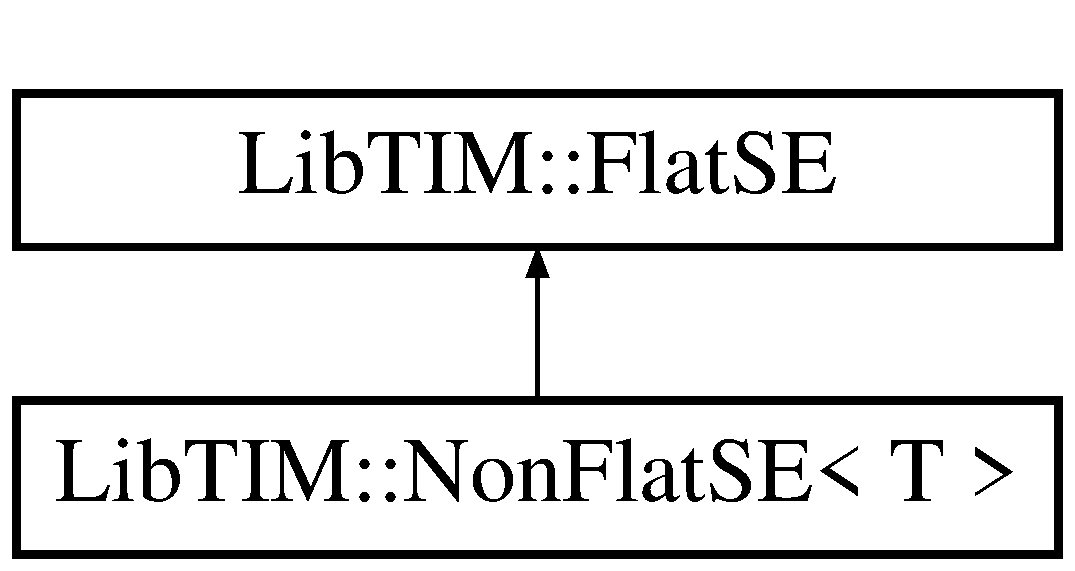
\includegraphics[height=2cm]{classLibTIM_1_1FlatSE}
\end{center}
\end{figure}
\subsection*{Public Types}
\begin{CompactItemize}
\item 
typedef std::vector$<$ {\bf Point}$<$ {\bf TCoord} $>$ $>$::{\bf iterator} {\bf iterator\_\-point}
\item 
typedef std::vector$<$ {\bf TOffset} $>$::{\bf iterator} {\bf iterator\_\-offset}
\item 
typedef {\bf iterator\_\-offset} {\bf iterator}
\end{CompactItemize}
\subsection*{Public Member Functions}
\begin{CompactItemize}
\item 
{\bf Flat\-SE} ()
\item 
{\bf Flat\-SE} (const {\bf Image}$<$ {\bf U8} $>$ \&im)
\item 
{\bf Flat\-SE} \& {\bf Flat\-SE::operator=} (const {\bf Flat\-SE} \&se)
\item 
{\bf Flat\-SE} (const {\bf Flat\-SE} \&se)
\item 
int {\bf get\-Nb\-Points} () const 
\begin{CompactList}\small\item\em returns the number of points contained in the structuring element (cardinal of the set) \item\end{CompactList}\item 
void {\bf set\-Context} (const {\bf TSize} $\ast$size)
\begin{CompactList}\small\item\em computes the offset of each point, according to \char`\"{}size\char`\"{} \item\end{CompactList}\item 
{\bf Point}$<$ {\bf TCoord} $>$ {\bf get\-Point} (int i) const 
\item 
void {\bf add\-Point} ({\bf Point}$<$ {\bf TCoord} $>$ p)
\item 
{\bf TOffset} {\bf get\-Offset} (int point)
\begin{CompactList}\small\item\em returns the offset of \char`\"{}point\char`\"{} \item\end{CompactList}\item 
{\bf TCoord} $\ast$ {\bf get\-Negative\-Offsets} ()
\item 
{\bf TCoord} $\ast$ {\bf get\-Positive\-Offsets} ()
\item 
void {\bf make\-Symmetric} ()
\item 
{\bf Image}$<$ {\bf U8} $>$ {\bf Flat\-SE::to\-Image} ()
\item 
{\bf Flat\-SE} \& {\bf operator+=} ({\bf Flat\-SE} \&b)
\item 
{\bf iterator} {\bf begin} ()
\item 
{\bf iterator} {\bf end} ()
\item 
{\bf iterator\_\-point} {\bf begin\_\-point} ()
\item 
{\bf iterator\_\-point} {\bf end\_\-point} ()
\item 
void {\bf make2DN4} ()
\begin{CompactList}\small\item\em Basic neighborhoods in 2D N4 and N8. \item\end{CompactList}\item 
void {\bf make2DN8} ()
\item 
void {\bf make2DN9} ()
\begin{CompactList}\small\item\em same as before but includes origin \item\end{CompactList}\item 
void {\bf make3DN6} ()
\begin{CompactList}\small\item\em In 3D N6,18,26. \item\end{CompactList}\item 
void {\bf make3DN18} ()
\item 
void {\bf make3DN26} ()
\item 
template$<$class Voxel\-Type$>$ void {\bf make\-Ball\-Euclidian2D} ({\bf Image}$<$ Voxel\-Type $>$ \&img, double r)
\item 
template$<$class Voxel\-Type$>$ void {\bf make\-Ball\-Chessboard2D} ({\bf Image}$<$ Voxel\-Type $>$ \&img, double rx, double ry)
\item 
template$<$class Voxel\-Type$>$ void {\bf make\-Ball\-Euclidian3D} ({\bf Image}$<$ Voxel\-Type $>$ \&img, double r)
\item 
template$<$class Voxel\-Type$>$ void {\bf make\-Circle2D} ({\bf Image}$<$ Voxel\-Type $>$ \&img, double r, double t)
\begin{CompactList}\small\item\em circle with specified thickness \item\end{CompactList}\item 
void {\bf print} ()
\item 
void {\bf reserve} (size\_\-t size)
\item 
void {\bf clear} ()
\end{CompactItemize}
\subsection*{Protected Attributes}
\begin{CompactItemize}
\item 
std::vector$<$ {\bf Point}$<$ {\bf TCoord} $>$ $>$ {\bf points}
\item 
std::vector$<$ {\bf TOffset} $>$ {\bf offsets}
\end{CompactItemize}


\subsection{Detailed Description}
Container base class for flat structuring elements (or binary masks). 

\begin{Desc}
\item[Example:]

\footnotesize\begin{verbatim}	FlatSE se;
	se.make2DN9();
	\end{verbatim}
\normalsize
 creates a 2D structuring element containing a 3x3 square. The origin is at the center. 

\footnotesize\begin{verbatim}	FlatSE se;
	se.makeBallEuclidian2D(r, im);
	\end{verbatim}
\normalsize
 creates 2D structuring element containing a ball of radius r according to the voxels spacing of im. The origin is at the center.\end{Desc}
WARNING: some algorithms require a {\em connexity\/} rather than a structuring element in parameters. To this end, use for example {\bf make2DN8()}{\rm (p.\,\pageref{classLibTIM_1_1FlatSE_a19})} to compute a 8-neighborhood (now the center is {\em not\/} included in the structuring element) Adding a {\em connexity\/} structure is in project.



\subsection{Member Typedef Documentation}
\index{LibTIM::FlatSE@{Lib\-TIM::Flat\-SE}!iterator@{iterator}}
\index{iterator@{iterator}!LibTIM::FlatSE@{Lib\-TIM::Flat\-SE}}
\subsubsection{\setlength{\rightskip}{0pt plus 5cm}typedef {\bf iterator\_\-offset} {\bf Lib\-TIM::Flat\-SE::iterator}}\label{classLibTIM_1_1FlatSE_w2}


\index{LibTIM::FlatSE@{Lib\-TIM::Flat\-SE}!iterator_offset@{iterator\_\-offset}}
\index{iterator_offset@{iterator\_\-offset}!LibTIM::FlatSE@{Lib\-TIM::Flat\-SE}}
\subsubsection{\setlength{\rightskip}{0pt plus 5cm}typedef std::vector$<${\bf TOffset} $>$::{\bf iterator} {\bf Lib\-TIM::Flat\-SE::iterator\_\-offset}}\label{classLibTIM_1_1FlatSE_w1}


\index{LibTIM::FlatSE@{Lib\-TIM::Flat\-SE}!iterator_point@{iterator\_\-point}}
\index{iterator_point@{iterator\_\-point}!LibTIM::FlatSE@{Lib\-TIM::Flat\-SE}}
\subsubsection{\setlength{\rightskip}{0pt plus 5cm}typedef std::vector$<${\bf Point}$<${\bf TCoord}$>$ $>$::{\bf iterator} {\bf Lib\-TIM::Flat\-SE::iterator\_\-point}}\label{classLibTIM_1_1FlatSE_w0}




\subsection{Constructor \& Destructor Documentation}
\index{LibTIM::FlatSE@{Lib\-TIM::Flat\-SE}!FlatSE@{FlatSE}}
\index{FlatSE@{FlatSE}!LibTIM::FlatSE@{Lib\-TIM::Flat\-SE}}
\subsubsection{\setlength{\rightskip}{0pt plus 5cm}Lib\-TIM::Flat\-SE::Flat\-SE ()\hspace{0.3cm}{\tt  [inline]}}\label{classLibTIM_1_1FlatSE_a0}


\index{LibTIM::FlatSE@{Lib\-TIM::Flat\-SE}!FlatSE@{FlatSE}}
\index{FlatSE@{FlatSE}!LibTIM::FlatSE@{Lib\-TIM::Flat\-SE}}
\subsubsection{\setlength{\rightskip}{0pt plus 5cm}Lib\-TIM::Flat\-SE::Flat\-SE (const {\bf Image}$<$ {\bf U8} $>$ \& {\em im})}\label{classLibTIM_1_1FlatSE_a1}


\index{LibTIM::FlatSE@{Lib\-TIM::Flat\-SE}!FlatSE@{FlatSE}}
\index{FlatSE@{FlatSE}!LibTIM::FlatSE@{Lib\-TIM::Flat\-SE}}
\subsubsection{\setlength{\rightskip}{0pt plus 5cm}Lib\-TIM::Flat\-SE::Flat\-SE (const {\bf Flat\-SE} \& {\em se})\hspace{0.3cm}{\tt  [inline]}}\label{classLibTIM_1_1FlatSE_a3}




\subsection{Member Function Documentation}
\index{LibTIM::FlatSE@{Lib\-TIM::Flat\-SE}!addPoint@{addPoint}}
\index{addPoint@{addPoint}!LibTIM::FlatSE@{Lib\-TIM::Flat\-SE}}
\subsubsection{\setlength{\rightskip}{0pt plus 5cm}void Lib\-TIM::Flat\-SE::add\-Point ({\bf Point}$<$ {\bf TCoord} $>$ {\em p})\hspace{0.3cm}{\tt  [inline]}}\label{classLibTIM_1_1FlatSE_a7}


\index{LibTIM::FlatSE@{Lib\-TIM::Flat\-SE}!begin@{begin}}
\index{begin@{begin}!LibTIM::FlatSE@{Lib\-TIM::Flat\-SE}}
\subsubsection{\setlength{\rightskip}{0pt plus 5cm}{\bf iterator} Lib\-TIM::Flat\-SE::begin ()\hspace{0.3cm}{\tt  [inline]}}\label{classLibTIM_1_1FlatSE_a14}


\index{LibTIM::FlatSE@{Lib\-TIM::Flat\-SE}!begin_point@{begin\_\-point}}
\index{begin_point@{begin\_\-point}!LibTIM::FlatSE@{Lib\-TIM::Flat\-SE}}
\subsubsection{\setlength{\rightskip}{0pt plus 5cm}{\bf iterator\_\-point} Lib\-TIM::Flat\-SE::begin\_\-point ()\hspace{0.3cm}{\tt  [inline]}}\label{classLibTIM_1_1FlatSE_a16}


\index{LibTIM::FlatSE@{Lib\-TIM::Flat\-SE}!clear@{clear}}
\index{clear@{clear}!LibTIM::FlatSE@{Lib\-TIM::Flat\-SE}}
\subsubsection{\setlength{\rightskip}{0pt plus 5cm}void Lib\-TIM::Flat\-SE::clear ()\hspace{0.3cm}{\tt  [inline]}}\label{classLibTIM_1_1FlatSE_a30}




Reimplemented in {\bf Lib\-TIM::Non\-Flat\-SE$<$ T $>$} {\rm (p.\,\pageref{classLibTIM_1_1NonFlatSE_a10})}.\index{LibTIM::FlatSE@{Lib\-TIM::Flat\-SE}!end@{end}}
\index{end@{end}!LibTIM::FlatSE@{Lib\-TIM::Flat\-SE}}
\subsubsection{\setlength{\rightskip}{0pt plus 5cm}{\bf iterator} Lib\-TIM::Flat\-SE::end ()\hspace{0.3cm}{\tt  [inline]}}\label{classLibTIM_1_1FlatSE_a15}


\index{LibTIM::FlatSE@{Lib\-TIM::Flat\-SE}!end_point@{end\_\-point}}
\index{end_point@{end\_\-point}!LibTIM::FlatSE@{Lib\-TIM::Flat\-SE}}
\subsubsection{\setlength{\rightskip}{0pt plus 5cm}{\bf iterator\_\-point} Lib\-TIM::Flat\-SE::end\_\-point ()\hspace{0.3cm}{\tt  [inline]}}\label{classLibTIM_1_1FlatSE_a17}


\index{LibTIM::FlatSE@{Lib\-TIM::Flat\-SE}!FlatSE::operator=@{FlatSE::operator=}}
\index{FlatSE::operator=@{FlatSE::operator=}!LibTIM::FlatSE@{Lib\-TIM::Flat\-SE}}
\subsubsection{\setlength{\rightskip}{0pt plus 5cm}{\bf Flat\-SE}\& Lib\-TIM::Flat\-SE::Flat\-SE::operator= (const {\bf Flat\-SE} \& {\em se})}\label{classLibTIM_1_1FlatSE_a2}


\index{LibTIM::FlatSE@{Lib\-TIM::Flat\-SE}!FlatSE::toImage@{FlatSE::toImage}}
\index{FlatSE::toImage@{FlatSE::toImage}!LibTIM::FlatSE@{Lib\-TIM::Flat\-SE}}
\subsubsection{\setlength{\rightskip}{0pt plus 5cm}{\bf Image}$<${\bf U8}$>$ Lib\-TIM::Flat\-SE::Flat\-SE::to\-Image ()}\label{classLibTIM_1_1FlatSE_a12}


\index{LibTIM::FlatSE@{Lib\-TIM::Flat\-SE}!getNbPoints@{getNbPoints}}
\index{getNbPoints@{getNbPoints}!LibTIM::FlatSE@{Lib\-TIM::Flat\-SE}}
\subsubsection{\setlength{\rightskip}{0pt plus 5cm}int Lib\-TIM::Flat\-SE::get\-Nb\-Points () const\hspace{0.3cm}{\tt  [inline]}}\label{classLibTIM_1_1FlatSE_a4}


returns the number of points contained in the structuring element (cardinal of the set) 

\index{LibTIM::FlatSE@{Lib\-TIM::Flat\-SE}!getNegativeOffsets@{getNegativeOffsets}}
\index{getNegativeOffsets@{getNegativeOffsets}!LibTIM::FlatSE@{Lib\-TIM::Flat\-SE}}
\subsubsection{\setlength{\rightskip}{0pt plus 5cm}{\bf TCoord} $\ast$ Lib\-TIM::Flat\-SE::get\-Negative\-Offsets ()\hspace{0.3cm}{\tt  [inline]}}\label{classLibTIM_1_1FlatSE_a9}


\index{LibTIM::FlatSE@{Lib\-TIM::Flat\-SE}!getOffset@{getOffset}}
\index{getOffset@{getOffset}!LibTIM::FlatSE@{Lib\-TIM::Flat\-SE}}
\subsubsection{\setlength{\rightskip}{0pt plus 5cm}{\bf TOffset} Lib\-TIM::Flat\-SE::get\-Offset (int {\em point})\hspace{0.3cm}{\tt  [inline]}}\label{classLibTIM_1_1FlatSE_a8}


returns the offset of \char`\"{}point\char`\"{} 

\index{LibTIM::FlatSE@{Lib\-TIM::Flat\-SE}!getPoint@{getPoint}}
\index{getPoint@{getPoint}!LibTIM::FlatSE@{Lib\-TIM::Flat\-SE}}
\subsubsection{\setlength{\rightskip}{0pt plus 5cm}{\bf Point}$<${\bf TCoord}$>$ Lib\-TIM::Flat\-SE::get\-Point (int {\em i}) const\hspace{0.3cm}{\tt  [inline]}}\label{classLibTIM_1_1FlatSE_a6}


\index{LibTIM::FlatSE@{Lib\-TIM::Flat\-SE}!getPositiveOffsets@{getPositiveOffsets}}
\index{getPositiveOffsets@{getPositiveOffsets}!LibTIM::FlatSE@{Lib\-TIM::Flat\-SE}}
\subsubsection{\setlength{\rightskip}{0pt plus 5cm}{\bf TCoord} $\ast$ Lib\-TIM::Flat\-SE::get\-Positive\-Offsets ()\hspace{0.3cm}{\tt  [inline]}}\label{classLibTIM_1_1FlatSE_a10}


\index{LibTIM::FlatSE@{Lib\-TIM::Flat\-SE}!make2DN4@{make2DN4}}
\index{make2DN4@{make2DN4}!LibTIM::FlatSE@{Lib\-TIM::Flat\-SE}}
\subsubsection{\setlength{\rightskip}{0pt plus 5cm}void Lib\-TIM::Flat\-SE::make2DN4 ()\hspace{0.3cm}{\tt  [inline]}}\label{classLibTIM_1_1FlatSE_a18}


Basic neighborhoods in 2D N4 and N8. 

Basic neighborhood (4-neighborhood). Warning: do not contain the origin!\index{LibTIM::FlatSE@{Lib\-TIM::Flat\-SE}!make2DN8@{make2DN8}}
\index{make2DN8@{make2DN8}!LibTIM::FlatSE@{Lib\-TIM::Flat\-SE}}
\subsubsection{\setlength{\rightskip}{0pt plus 5cm}void Lib\-TIM::Flat\-SE::make2DN8 ()\hspace{0.3cm}{\tt  [inline]}}\label{classLibTIM_1_1FlatSE_a19}


Basic neighborhood (8-neighborhood). Warning: do not contain the origin!\index{LibTIM::FlatSE@{Lib\-TIM::Flat\-SE}!make2DN9@{make2DN9}}
\index{make2DN9@{make2DN9}!LibTIM::FlatSE@{Lib\-TIM::Flat\-SE}}
\subsubsection{\setlength{\rightskip}{0pt plus 5cm}void Lib\-TIM::Flat\-SE::make2DN9 ()\hspace{0.3cm}{\tt  [inline]}}\label{classLibTIM_1_1FlatSE_a20}


same as before but includes origin 

\index{LibTIM::FlatSE@{Lib\-TIM::Flat\-SE}!make3DN18@{make3DN18}}
\index{make3DN18@{make3DN18}!LibTIM::FlatSE@{Lib\-TIM::Flat\-SE}}
\subsubsection{\setlength{\rightskip}{0pt plus 5cm}void Lib\-TIM::Flat\-SE::make3DN18 ()}\label{classLibTIM_1_1FlatSE_a22}


\index{LibTIM::FlatSE@{Lib\-TIM::Flat\-SE}!make3DN26@{make3DN26}}
\index{make3DN26@{make3DN26}!LibTIM::FlatSE@{Lib\-TIM::Flat\-SE}}
\subsubsection{\setlength{\rightskip}{0pt plus 5cm}void Lib\-TIM::Flat\-SE::make3DN26 ()}\label{classLibTIM_1_1FlatSE_a23}


\index{LibTIM::FlatSE@{Lib\-TIM::Flat\-SE}!make3DN6@{make3DN6}}
\index{make3DN6@{make3DN6}!LibTIM::FlatSE@{Lib\-TIM::Flat\-SE}}
\subsubsection{\setlength{\rightskip}{0pt plus 5cm}void Lib\-TIM::Flat\-SE::make3DN6 ()}\label{classLibTIM_1_1FlatSE_a21}


In 3D N6,18,26. 

\index{LibTIM::FlatSE@{Lib\-TIM::Flat\-SE}!makeBallChessboard2D@{makeBallChessboard2D}}
\index{makeBallChessboard2D@{makeBallChessboard2D}!LibTIM::FlatSE@{Lib\-TIM::Flat\-SE}}
\subsubsection{\setlength{\rightskip}{0pt plus 5cm}template$<$class Voxel\-Type$>$ void Lib\-TIM::Flat\-SE::make\-Ball\-Chessboard2D ({\bf Image}$<$ Voxel\-Type $>$ \& {\em img}, double {\em rx}, double {\em ry})}\label{classLibTIM_1_1FlatSE_a25}


\index{LibTIM::FlatSE@{Lib\-TIM::Flat\-SE}!makeBallEuclidian2D@{makeBallEuclidian2D}}
\index{makeBallEuclidian2D@{makeBallEuclidian2D}!LibTIM::FlatSE@{Lib\-TIM::Flat\-SE}}
\subsubsection{\setlength{\rightskip}{0pt plus 5cm}template$<$class Voxel\-Type$>$ void Lib\-TIM::Flat\-SE::make\-Ball\-Euclidian2D ({\bf Image}$<$ Voxel\-Type $>$ \& {\em img}, double {\em r})}\label{classLibTIM_1_1FlatSE_a24}


\index{LibTIM::FlatSE@{Lib\-TIM::Flat\-SE}!makeBallEuclidian3D@{makeBallEuclidian3D}}
\index{makeBallEuclidian3D@{makeBallEuclidian3D}!LibTIM::FlatSE@{Lib\-TIM::Flat\-SE}}
\subsubsection{\setlength{\rightskip}{0pt plus 5cm}template$<$class Voxel\-Type$>$ void Lib\-TIM::Flat\-SE::make\-Ball\-Euclidian3D ({\bf Image}$<$ Voxel\-Type $>$ \& {\em img}, double {\em r})}\label{classLibTIM_1_1FlatSE_a26}


\index{LibTIM::FlatSE@{Lib\-TIM::Flat\-SE}!makeCircle2D@{makeCircle2D}}
\index{makeCircle2D@{makeCircle2D}!LibTIM::FlatSE@{Lib\-TIM::Flat\-SE}}
\subsubsection{\setlength{\rightskip}{0pt plus 5cm}template$<$class T$>$ void Lib\-TIM::Flat\-SE::make\-Circle2D ({\bf Image}$<$ Voxel\-Type $>$ \& {\em img}, double {\em r}, double {\em t})}\label{classLibTIM_1_1FlatSE_a27}


circle with specified thickness 

\index{LibTIM::FlatSE@{Lib\-TIM::Flat\-SE}!makeSymmetric@{makeSymmetric}}
\index{makeSymmetric@{makeSymmetric}!LibTIM::FlatSE@{Lib\-TIM::Flat\-SE}}
\subsubsection{\setlength{\rightskip}{0pt plus 5cm}void Lib\-TIM::Flat\-SE::make\-Symmetric ()\hspace{0.3cm}{\tt  [inline]}}\label{classLibTIM_1_1FlatSE_a11}


\index{LibTIM::FlatSE@{Lib\-TIM::Flat\-SE}!operator+=@{operator+=}}
\index{operator+=@{operator+=}!LibTIM::FlatSE@{Lib\-TIM::Flat\-SE}}
\subsubsection{\setlength{\rightskip}{0pt plus 5cm}{\bf Flat\-SE}\& Lib\-TIM::Flat\-SE::operator+= ({\bf Flat\-SE} \& {\em b})\hspace{0.3cm}{\tt  [inline]}}\label{classLibTIM_1_1FlatSE_a13}


\index{LibTIM::FlatSE@{Lib\-TIM::Flat\-SE}!print@{print}}
\index{print@{print}!LibTIM::FlatSE@{Lib\-TIM::Flat\-SE}}
\subsubsection{\setlength{\rightskip}{0pt plus 5cm}void Lib\-TIM::Flat\-SE::print ()\hspace{0.3cm}{\tt  [inline]}}\label{classLibTIM_1_1FlatSE_a28}




Reimplemented in {\bf Lib\-TIM::Non\-Flat\-SE$<$ T $>$} {\rm (p.\,\pageref{classLibTIM_1_1NonFlatSE_a8})}.\index{LibTIM::FlatSE@{Lib\-TIM::Flat\-SE}!reserve@{reserve}}
\index{reserve@{reserve}!LibTIM::FlatSE@{Lib\-TIM::Flat\-SE}}
\subsubsection{\setlength{\rightskip}{0pt plus 5cm}void Lib\-TIM::Flat\-SE::reserve (size\_\-t {\em size})\hspace{0.3cm}{\tt  [inline]}}\label{classLibTIM_1_1FlatSE_a29}




Reimplemented in {\bf Lib\-TIM::Non\-Flat\-SE$<$ T $>$} {\rm (p.\,\pageref{classLibTIM_1_1NonFlatSE_a9})}.\index{LibTIM::FlatSE@{Lib\-TIM::Flat\-SE}!setContext@{setContext}}
\index{setContext@{setContext}!LibTIM::FlatSE@{Lib\-TIM::Flat\-SE}}
\subsubsection{\setlength{\rightskip}{0pt plus 5cm}void Lib\-TIM::Flat\-SE::set\-Context (const {\bf TSize} $\ast$ {\em size})\hspace{0.3cm}{\tt  [inline]}}\label{classLibTIM_1_1FlatSE_a5}


computes the offset of each point, according to \char`\"{}size\char`\"{} 



\subsection{Member Data Documentation}
\index{LibTIM::FlatSE@{Lib\-TIM::Flat\-SE}!offsets@{offsets}}
\index{offsets@{offsets}!LibTIM::FlatSE@{Lib\-TIM::Flat\-SE}}
\subsubsection{\setlength{\rightskip}{0pt plus 5cm}std::vector$<${\bf TOffset}$>$ {\bf Lib\-TIM::Flat\-SE::offsets}\hspace{0.3cm}{\tt  [protected]}}\label{classLibTIM_1_1FlatSE_p1}


\index{LibTIM::FlatSE@{Lib\-TIM::Flat\-SE}!points@{points}}
\index{points@{points}!LibTIM::FlatSE@{Lib\-TIM::Flat\-SE}}
\subsubsection{\setlength{\rightskip}{0pt plus 5cm}std::vector$<${\bf Point}$<${\bf TCoord}$>$ $>$ {\bf Lib\-TIM::Flat\-SE::points}\hspace{0.3cm}{\tt  [protected]}}\label{classLibTIM_1_1FlatSE_p0}




The documentation for this class was generated from the following files:\begin{CompactItemize}
\item 
Common/{\bf Flat\-SE.h}\item 
Common/{\bf Flat\-SE.hxx}\end{CompactItemize}

\section{Lib\-TIM::Histogram$<$ T $>$ Class Template Reference}
\label{classLibTIM_1_1Histogram}\index{LibTIM::Histogram@{LibTIM::Histogram}}
Container for histograms.  


{\tt \#include $<$Histogram.h$>$}

\subsection*{Public Member Functions}
\begin{CompactItemize}
\item 
{\bf Histogram} ({\bf Image}$<$ T $>$ \&im)
\begin{CompactList}\small\item\em Constructs an histogram from image im. \item\end{CompactList}\item 
void {\bf write} (const char $\ast$filename)
\begin{CompactList}\small\item\em Write histogram into file. \item\end{CompactList}\end{CompactItemize}


\subsection{Detailed Description}
\subsubsection*{template$<$class T$>$ class Lib\-TIM::Histogram$<$ T $>$}

Container for histograms. 

Structure describing an histogram. {\bf Histogram}{\rm (p.\,\pageref{classLibTIM_1_1Histogram})} can be constructed from an {\bf Image}{\rm (p.\,\pageref{classLibTIM_1_1Image})}



\subsection{Constructor \& Destructor Documentation}
\index{LibTIM::Histogram@{Lib\-TIM::Histogram}!Histogram@{Histogram}}
\index{Histogram@{Histogram}!LibTIM::Histogram@{Lib\-TIM::Histogram}}
\subsubsection{\setlength{\rightskip}{0pt plus 5cm}template$<$class T$>$ {\bf Lib\-TIM::Histogram}$<$ T $>$::{\bf Histogram} ({\bf Image}$<$ T $>$ \& {\em im})}\label{classLibTIM_1_1Histogram_a0}


Constructs an histogram from image im. 



\subsection{Member Function Documentation}
\index{LibTIM::Histogram@{Lib\-TIM::Histogram}!write@{write}}
\index{write@{write}!LibTIM::Histogram@{Lib\-TIM::Histogram}}
\subsubsection{\setlength{\rightskip}{0pt plus 5cm}template$<$class T$>$ void {\bf Lib\-TIM::Histogram}$<$ T $>$::write (const char $\ast$ {\em filename})}\label{classLibTIM_1_1Histogram_a1}


Write histogram into file. 

{\bf Histogram}{\rm (p.\,\pageref{classLibTIM_1_1Histogram})} is writed in a text file (xmgrace format)

The documentation for this class was generated from the following files:\begin{CompactItemize}
\item 
Common/{\bf Histogram.h}\item 
Common/{\bf Histogram.hxx}\end{CompactItemize}

\section{Lib\-TIM::Image$<$ T $>$ Class Template Reference}
\label{classLibTIM_1_1Image}\index{LibTIM::Image@{LibTIM::Image}}
Container base for images of generic type T in {\bf Lib\-TIM}{\rm (p.\,\pageref{namespaceLibTIM})}.  


{\tt \#include $<$Image.h$>$}

\subsection*{Public Types}
\begin{CompactItemize}
\item 
typedef {\bf Image\-Iterator}$<$ {\bf Image}, T $>$ {\bf iterator}
\begin{CompactList}\small\item\em Iterators. \item\end{CompactList}\item 
typedef {\bf Image\-Iterator}$<$ const {\bf Image}, const T $>$ {\bf const\_\-iterator}
\item 
typedef {\bf Image\-Iterator\-XYZ}$<$ {\bf Image}, T $>$ {\bf iterator\-XYZ}
\item 
typedef {\bf Image\-Iterator\-XYZ}$<$ const {\bf Image}, const T $>$ {\bf const\_\-iterator\-XYZ}
\item 
typedef std::reverse\_\-iterator$<$ {\bf const\_\-iterator} $>$ {\bf const\_\-reverse\_\-iterator}
\item 
typedef std::reverse\_\-iterator$<$ {\bf iterator} $>$ {\bf reverse\_\-iterator}
\end{CompactItemize}
\subsection*{Public Member Functions}
\begin{CompactItemize}
\item 
void {\bf save} (const char $\ast$filename)
\begin{CompactList}\small\item\em Save image file. \item\end{CompactList}\item 
{\bf Image} (const {\bf TSize} $\ast$size)
\begin{CompactList}\small\item\em Constructors. \item\end{CompactList}\item 
{\bf Image} (const {\bf TSize} x\-Size=1, const {\bf TSize} y\-Size=1, const {\bf TSize} z\-Size=1)
\item 
{\bf Image} (const {\bf TSize} $\ast$size, const {\bf TSpacing} $\ast$spacing, const T $\ast$data)
\item 
{\bf $\sim$Image} ()
\begin{CompactList}\small\item\em Destructor (delete the buffer). \item\end{CompactList}\item 
{\bf Image} (const {\bf Image}$<$ T $>$ \&im)
\begin{CompactList}\small\item\em Copy constructor. \item\end{CompactList}\item 
{\bf Image}$<$ T $>$ \& {\bf operator=} (const {\bf Image}$<$ T $>$ \&im)
\begin{CompactList}\small\item\em Assignment operator. \item\end{CompactList}\item 
template$<$class T2$>$ {\bf Image} (const {\bf Image}$<$ T2 $>$ \&im)
\begin{CompactList}\small\item\em Type conversion. \item\end{CompactList}\item 
{\bf TSize} $\ast$ {\bf get\-Size} () const 
\item 
{\bf TSize} {\bf get\-Size\-X} () const 
\item 
{\bf TSize} {\bf get\-Size\-Y} () const 
\item 
{\bf TSize} {\bf get\-Size\-Z} () const 
\item 
void {\bf set\-Size} ({\bf TSize} $\ast$size)
\item 
void {\bf set\-Size} ({\bf TSize} x, {\bf TSize} y, {\bf TSize} z)
\item 
{\bf TSpacing} $\ast$ {\bf get\-Spacing} ()
\item 
{\bf TSpacing} {\bf get\-Spacing\-X} () const 
\item 
{\bf TSpacing} {\bf get\-Spacing\-Y} () const 
\item 
{\bf TSpacing} {\bf get\-Spacing\-Z} () const 
\item 
void {\bf set\-Spacing\-X} ({\bf TSpacing} vx)
\item 
void {\bf set\-Spacing\-Y} ({\bf TSpacing} vy)
\item 
void {\bf set\-Spacing\-Z} ({\bf TSpacing} vz)
\item 
{\bf TOffset} {\bf get\-Buf\-Size} () const 
\item 
T $\ast$ {\bf get\-Data} ()
\item 
{\bf iterator} {\bf begin} ()
\item 
{\bf const\_\-iterator} {\bf begin} () const 
\item 
{\bf iterator} {\bf end} ()
\item 
{\bf const\_\-iterator} {\bf end} () const 
\item 
{\bf reverse\_\-iterator} {\bf rbegin} ()
\item 
{\bf const\_\-reverse\_\-iterator} {\bf rbegin} () const 
\item 
{\bf reverse\_\-iterator} {\bf rend} ()
\item 
{\bf const\_\-reverse\_\-iterator} {\bf rend} () const 
\item 
T \& {\bf operator()} ({\bf TCoord} x, {\bf TCoord} y, {\bf TCoord} z=0)
\begin{CompactList}\small\item\em Coordinates write version. \item\end{CompactList}\item 
T {\bf operator()} ({\bf TCoord} x, {\bf TCoord} y, {\bf TCoord} z=0) const 
\begin{CompactList}\small\item\em Coordinates read-only version. \item\end{CompactList}\item 
T \& {\bf operator()} ({\bf TOffset} offset)
\begin{CompactList}\small\item\em Offset write version. \item\end{CompactList}\item 
T {\bf operator()} ({\bf TOffset} offset) const 
\begin{CompactList}\small\item\em Offset read-only version. \item\end{CompactList}\item 
T \& {\bf operator()} ({\bf Point}$<$ {\bf TCoord} $>$ p)
\begin{CompactList}\small\item\em {\bf Point}{\rm (p.\,\pageref{classLibTIM_1_1Point})} write version. \item\end{CompactList}\item 
T {\bf operator()} ({\bf Point}$<$ {\bf TCoord} $>$ p) const 
\begin{CompactList}\small\item\em {\bf Point}{\rm (p.\,\pageref{classLibTIM_1_1Point})} read-only version. \item\end{CompactList}\item 
{\bf Image} \& {\bf operator+=} ({\bf Image}$<$ T $>$ \&op)
\begin{CompactList}\small\item\em {\bf Image}{\rm (p.\,\pageref{classLibTIM_1_1Image})} operators. \item\end{CompactList}\item 
{\bf Image} \& {\bf operator-=} ({\bf Image}$<$ T $>$ \&op)
\item 
{\bf Image} \& {\bf operator $\ast$=} ({\bf Image}$<$ T $>$ \&op)
\item 
{\bf Image} \& {\bf operator/=} ({\bf Image}$<$ T $>$ \&op)
\item 
{\bf Image} \& {\bf operator \&=} ({\bf Image}$<$ T $>$ \&op)
\begin{CompactList}\small\item\em Pointwise minimum and maximum. \item\end{CompactList}\item 
{\bf Image} \& {\bf operator$|$=} ({\bf Image}$<$ T $>$ \&op)
\item 
{\bf Image} \& {\bf operator!} (void)
\begin{CompactList}\small\item\em Negative. \item\end{CompactList}\item 
bool {\bf operator==} ({\bf Image}$<$ T $>$ \&op)
\item 
template$<$class T2$>$ void {\bf set\-Image\-Infos} ({\bf Image}$<$ T2 $>$ \&im)
\item 
T {\bf get\-Max} () const 
\begin{CompactList}\small\item\em Min and max. \item\end{CompactList}\item 
T {\bf get\-Min} () const 
\item 
void {\bf fill} (const T value)
\begin{CompactList}\small\item\em {\bf Image}{\rm (p.\,\pageref{classLibTIM_1_1Image})} misc. \item\end{CompactList}\item 
{\bf Image}$<$ T $>$ {\bf crop} (const {\bf TCoord} from\-X=0, const {\bf TCoord} to\-X=1, const {\bf TCoord} from\-Y=0, const {\bf TCoord} to\-Y=1, const {\bf TCoord} from\-Z=0, const {\bf TCoord} to\-Z=1)
\item 
void {\bf copy} ({\bf Image}$<$ T $>$ \&im, {\bf TCoord} x1, {\bf TCoord} y1, {\bf TCoord} z1, {\bf TCoord} x2, {\bf TCoord} y2, {\bf TCoord} z2, {\bf TCoord} px, {\bf TCoord} py, {\bf TCoord} pz)
\item 
void {\bf copy\-Fast} ({\bf Image}$<$ T $>$ \&im, int x1, int y1, int z1, int x2, int y2, int z2, int px, int py, int pz)
\item 
void {\bf copy\-Fast} ({\bf Image}$<$ T $>$ \&im, {\bf TCoord} px, {\bf TCoord} py, {\bf TCoord} pz)
\item 
void {\bf copy} ({\bf Image}$<$ T $>$ \&im, {\bf TCoord} px, {\bf TCoord} py, {\bf TCoord} pz)
\item 
void {\bf enlarge} ()
\item 
int {\bf get\-Offset} (int x, int y, int z)
\item 
{\bf Image}$<$ T $>$ {\bf get\-Reflection} ()
\item 
void {\bf print} ()
\item 
bool {\bf is\-Pos\-Valid} ({\bf TCoord} x, {\bf TCoord} y, {\bf TCoord} z=0) const 
\item 
bool {\bf is\-Pos\-Valid} ({\bf TOffset} offset) const 
\item 
bool {\bf is\-Pos\-Valid} ({\bf Point}$<$ {\bf TCoord} $>$ p) const 
\item 
template$<$$>$ int {\bf load} (const char $\ast$filename, {\bf Image}$<$ {\bf U8} $>$ \&im)
\item 
template$<$$>$ int {\bf load} (const char $\ast$filename, {\bf Image}$<$ {\bf U16} $>$ \&im)
\item 
template$<$$>$ int {\bf load} (const char $\ast$filename, {\bf Image}$<$ {\bf RGB} $>$ \&im)
\item 
template$<$$>$ void {\bf save} (const char $\ast$filename)
\item 
template$<$$>$ void {\bf save} (const char $\ast$filename)
\item 
template$<$$>$ void {\bf save} (const char $\ast$filename)
\end{CompactItemize}
\subsection*{Static Public Member Functions}
\begin{CompactItemize}
\item 
static int {\bf load} (const char $\ast$filename, {\bf Image}$<$ T $>$ \&im)
\begin{CompactList}\small\item\em {\bf Image}{\rm (p.\,\pageref{classLibTIM_1_1Image})} file loader. \item\end{CompactList}\end{CompactItemize}


\subsection{Detailed Description}
\subsubsection*{template$<$class T$>$ class Lib\-TIM::Image$<$ T $>$}

Container base for images of generic type T in {\bf Lib\-TIM}{\rm (p.\,\pageref{namespaceLibTIM})}. 

This structure represents the base image class of {\bf Lib\-TIM}{\rm (p.\,\pageref{namespaceLibTIM})}. It contains a buffer of elements of type T of size size[0]$\ast$size[1]$\ast$size[2] x,y and z voxels spacings are recorded in spacing[] \begin{Desc}
\item[Accessing elements]To access element (x,y,z) or offset (q), use: 

\footnotesize\begin{verbatim}val=im(x,y,z) \end{verbatim}
\normalsize
 

\footnotesize\begin{verbatim}val=im(q) \end{verbatim}
\normalsize
 To write element (x,y,z) or offset (q), use: 

\footnotesize\begin{verbatim}im(x,y,z)=val \end{verbatim}
\normalsize
 

\footnotesize\begin{verbatim}im(q)=val \end{verbatim}
\normalsize
\end{Desc}
\begin{Desc}
\item[Iterators]To iterate through elements, you should use iterators. There is two types of iterator: \begin{itemize}
\item 

\footnotesize\begin{verbatim}iterator \end{verbatim}
\normalsize
 to scan image in raster scan \item 

\footnotesize\begin{verbatim}reverse_iterator \end{verbatim}
\normalsize
 to scan image in anti-raster scan \item 

\footnotesize\begin{verbatim}iteratorXYZ \end{verbatim}
\normalsize
 to scan image in raster scan with the knowledge of coordinates \item 

\footnotesize\begin{verbatim}reverse_iteratorXYZ \end{verbatim}
\normalsize
 to scan image in anti-raster scan with the knowledge of coordinates\end{itemize}
{\bf begin()}{\rm (p.\,\pageref{group__Image_ga33})} and {\bf end()}{\rm (p.\,\pageref{group__Image_ga35})} methods return iterators on the beginning and the end of the {\bf Image}{\rm (p.\,\pageref{classLibTIM_1_1Image})} {\bf rbegin()}{\rm (p.\,\pageref{group__Image_ga37})} and {\bf rend()}{\rm (p.\,\pageref{group__Image_ga39})} methods are used with reverse\_\-iterators \end{Desc}
\begin{Desc}
\item[Example:]This piece of code initialized all elements of {\bf Image}{\rm (p.\,\pageref{classLibTIM_1_1Image})} to 0. (note that to do this you should better use the fill method) 

\footnotesize\begin{verbatim}	Image <U8> im;
	...
	Image<U8>::iterator it;
	Image<U8>::iterator end=im.end();
	for(it=im.begin(); it!=end; ++it)
		*it=0
	\end{verbatim}
\normalsize
\end{Desc}
Same thing with coordinates access (slower):



\footnotesize\begin{verbatim}	Image <U8> im;
	...
	Image<U8>::iteratorXYZ it;
	Image<U8>::iteratorXYZ end=im.end();
	for(it=im.begin(); it!=end; ++it)
		im(it.x,it.y,it.z)=0
	\end{verbatim}
\normalsize


Note that (as in these examples) it is faster to put im.end() in a variable.



\subsection{Member Function Documentation}
\index{LibTIM::Image@{Lib\-TIM::Image}!load@{load}}
\index{load@{load}!LibTIM::Image@{Lib\-TIM::Image}}
\subsubsection{\setlength{\rightskip}{0pt plus 5cm}template$<$$>$ int {\bf Lib\-TIM::Image}$<$ {\bf RGB} $>$::load (const char $\ast$ {\em filename}, {\bf Image}$<$ {\bf RGB} $>$ \& {\em im})\hspace{0.3cm}{\tt  [inline]}}\label{classLibTIM_1_1Image_a63}


\index{LibTIM::Image@{Lib\-TIM::Image}!load@{load}}
\index{load@{load}!LibTIM::Image@{Lib\-TIM::Image}}
\subsubsection{\setlength{\rightskip}{0pt plus 5cm}template$<$$>$ int {\bf Lib\-TIM::Image}$<$ {\bf U16} $>$::load (const char $\ast$ {\em filename}, {\bf Image}$<$ {\bf U16} $>$ \& {\em im})\hspace{0.3cm}{\tt  [inline]}}\label{classLibTIM_1_1Image_a62}


\index{LibTIM::Image@{Lib\-TIM::Image}!load@{load}}
\index{load@{load}!LibTIM::Image@{Lib\-TIM::Image}}
\subsubsection{\setlength{\rightskip}{0pt plus 5cm}template$<$$>$ int {\bf Lib\-TIM::Image}$<$ {\bf U8} $>$::load (const char $\ast$ {\em filename}, {\bf Image}$<$ {\bf U8} $>$ \& {\em im})\hspace{0.3cm}{\tt  [inline]}}\label{classLibTIM_1_1Image_a61}


\index{LibTIM::Image@{Lib\-TIM::Image}!save@{save}}
\index{save@{save}!LibTIM::Image@{Lib\-TIM::Image}}
\subsubsection{\setlength{\rightskip}{0pt plus 5cm}template$<$$>$ void {\bf Lib\-TIM::Image}$<$ {\bf RGB} $>$::save (const char $\ast$ {\em filename})\hspace{0.3cm}{\tt  [inline]}}\label{classLibTIM_1_1Image_a66}


\index{LibTIM::Image@{Lib\-TIM::Image}!save@{save}}
\index{save@{save}!LibTIM::Image@{Lib\-TIM::Image}}
\subsubsection{\setlength{\rightskip}{0pt plus 5cm}template$<$$>$ void {\bf Lib\-TIM::Image}$<$ {\bf U16} $>$::save (const char $\ast$ {\em filename})\hspace{0.3cm}{\tt  [inline]}}\label{classLibTIM_1_1Image_a65}


\index{LibTIM::Image@{Lib\-TIM::Image}!save@{save}}
\index{save@{save}!LibTIM::Image@{Lib\-TIM::Image}}
\subsubsection{\setlength{\rightskip}{0pt plus 5cm}template$<$$>$ void {\bf Lib\-TIM::Image}$<$ {\bf U8} $>$::save (const char $\ast$ {\em filename})\hspace{0.3cm}{\tt  [inline]}}\label{classLibTIM_1_1Image_a64}




The documentation for this class was generated from the following files:\begin{CompactItemize}
\item 
Common/{\bf Image.h}\item 
Common/{\bf Image.hxx}\end{CompactItemize}

\section{Lib\-TIM::Image\-Iterator$<$ TImage, T $>$ Class Template Reference}
\label{classLibTIM_1_1ImageIterator}\index{LibTIM::ImageIterator@{LibTIM::ImageIterator}}
{\tt \#include $<$Image\-Iterators.h$>$}

Inheritance diagram for Lib\-TIM::Image\-Iterator$<$ TImage, T $>$::\begin{figure}[H]
\begin{center}
\leavevmode
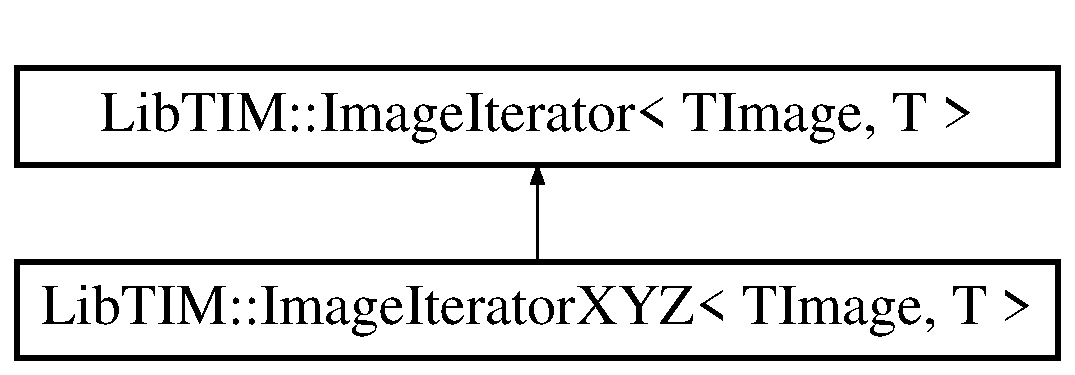
\includegraphics[height=2cm]{classLibTIM_1_1ImageIterator}
\end{center}
\end{figure}
\subsection*{Public Member Functions}
\begin{CompactItemize}
\item 
{\bf Image\-Iterator} ()
\item 
{\bf Image\-Iterator} (TImage $\ast${\bf im}, T $\ast$x)
\item 
T \& {\bf operator $\ast$} ()
\item 
T $\ast$ {\bf operator $\rightarrow$ } ()
\item 
{\bf Image\-Iterator}$<$ TImage, T $>$ \& {\bf operator++} ()
\item 
{\bf Image\-Iterator}$<$ TImage, T $>$ {\bf operator++} (int)
\item 
bool {\bf operator==} (const {\bf Image\-Iterator} \&x)
\item 
bool {\bf operator!=} (const {\bf Image\-Iterator} \&x)
\end{CompactItemize}
\subsection*{Public Attributes}
\begin{CompactItemize}
\item 
T $\ast$ {\bf ptr}
\item 
TImage $\ast$ {\bf im}
\end{CompactItemize}
\subsubsection*{template$<$class TImage, class T$>$ class Lib\-TIM::Image\-Iterator$<$ TImage, T $>$}



\subsection{Constructor \& Destructor Documentation}
\index{LibTIM::ImageIterator@{Lib\-TIM::Image\-Iterator}!ImageIterator@{ImageIterator}}
\index{ImageIterator@{ImageIterator}!LibTIM::ImageIterator@{Lib\-TIM::Image\-Iterator}}
\subsubsection{\setlength{\rightskip}{0pt plus 5cm}template$<$class TImage, class T$>$ {\bf Lib\-TIM::Image\-Iterator}$<$ TImage, T $>$::{\bf Image\-Iterator} ()\hspace{0.3cm}{\tt  [inline]}}\label{classLibTIM_1_1ImageIterator_a0}


\index{LibTIM::ImageIterator@{Lib\-TIM::Image\-Iterator}!ImageIterator@{ImageIterator}}
\index{ImageIterator@{ImageIterator}!LibTIM::ImageIterator@{Lib\-TIM::Image\-Iterator}}
\subsubsection{\setlength{\rightskip}{0pt plus 5cm}template$<$class TImage, class T$>$ {\bf Lib\-TIM::Image\-Iterator}$<$ TImage, T $>$::{\bf Image\-Iterator} (TImage $\ast$ {\em im}, T $\ast$ {\em x})\hspace{0.3cm}{\tt  [inline]}}\label{classLibTIM_1_1ImageIterator_a1}




\subsection{Member Function Documentation}
\index{LibTIM::ImageIterator@{Lib\-TIM::Image\-Iterator}!operator *@{operator $\ast$}}
\index{operator *@{operator $\ast$}!LibTIM::ImageIterator@{Lib\-TIM::Image\-Iterator}}
\subsubsection{\setlength{\rightskip}{0pt plus 5cm}template$<$class TImage, class T$>$ T\& {\bf Lib\-TIM::Image\-Iterator}$<$ TImage, T $>$::operator $\ast$ ()\hspace{0.3cm}{\tt  [inline]}}\label{classLibTIM_1_1ImageIterator_a2}




Reimplemented in {\bf Lib\-TIM::Image\-Iterator\-XYZ$<$ TImage, T $>$} {\rm (p.\,\pageref{classLibTIM_1_1ImageIteratorXYZ_a4})}.\index{LibTIM::ImageIterator@{Lib\-TIM::Image\-Iterator}!operator"!=@{operator"!=}}
\index{operator"!=@{operator"!=}!LibTIM::ImageIterator@{Lib\-TIM::Image\-Iterator}}
\subsubsection{\setlength{\rightskip}{0pt plus 5cm}template$<$class TImage, class T$>$ bool {\bf Lib\-TIM::Image\-Iterator}$<$ TImage, T $>$::operator!= (const {\bf Image\-Iterator}$<$ TImage, T $>$ \& {\em x})\hspace{0.3cm}{\tt  [inline]}}\label{classLibTIM_1_1ImageIterator_a7}


\index{LibTIM::ImageIterator@{Lib\-TIM::Image\-Iterator}!operator++@{operator++}}
\index{operator++@{operator++}!LibTIM::ImageIterator@{Lib\-TIM::Image\-Iterator}}
\subsubsection{\setlength{\rightskip}{0pt plus 5cm}template$<$class TImage, class T$>$ {\bf Image\-Iterator}$<$TImage, T$>$ {\bf Lib\-TIM::Image\-Iterator}$<$ TImage, T $>$::operator++ (int)\hspace{0.3cm}{\tt  [inline]}}\label{classLibTIM_1_1ImageIterator_a5}




Reimplemented in {\bf Lib\-TIM::Image\-Iterator\-XYZ$<$ TImage, T $>$} {\rm (p.\,\pageref{classLibTIM_1_1ImageIteratorXYZ_a7})}.\index{LibTIM::ImageIterator@{Lib\-TIM::Image\-Iterator}!operator++@{operator++}}
\index{operator++@{operator++}!LibTIM::ImageIterator@{Lib\-TIM::Image\-Iterator}}
\subsubsection{\setlength{\rightskip}{0pt plus 5cm}template$<$class TImage, class T$>$ {\bf Image\-Iterator}$<$TImage, T$>$\& {\bf Lib\-TIM::Image\-Iterator}$<$ TImage, T $>$::operator++ ()\hspace{0.3cm}{\tt  [inline]}}\label{classLibTIM_1_1ImageIterator_a4}




Reimplemented in {\bf Lib\-TIM::Image\-Iterator\-XYZ$<$ TImage, T $>$} {\rm (p.\,\pageref{classLibTIM_1_1ImageIteratorXYZ_a6})}.\index{LibTIM::ImageIterator@{Lib\-TIM::Image\-Iterator}!operator->@{operator-$>$}}
\index{operator->@{operator-$>$}!LibTIM::ImageIterator@{Lib\-TIM::Image\-Iterator}}
\subsubsection{\setlength{\rightskip}{0pt plus 5cm}template$<$class TImage, class T$>$ T$\ast$ {\bf Lib\-TIM::Image\-Iterator}$<$ TImage, T $>$::operator $\rightarrow$  ()\hspace{0.3cm}{\tt  [inline]}}\label{classLibTIM_1_1ImageIterator_a3}




Reimplemented in {\bf Lib\-TIM::Image\-Iterator\-XYZ$<$ TImage, T $>$} {\rm (p.\,\pageref{classLibTIM_1_1ImageIteratorXYZ_a5})}.\index{LibTIM::ImageIterator@{Lib\-TIM::Image\-Iterator}!operator==@{operator==}}
\index{operator==@{operator==}!LibTIM::ImageIterator@{Lib\-TIM::Image\-Iterator}}
\subsubsection{\setlength{\rightskip}{0pt plus 5cm}template$<$class TImage, class T$>$ bool {\bf Lib\-TIM::Image\-Iterator}$<$ TImage, T $>$::operator== (const {\bf Image\-Iterator}$<$ TImage, T $>$ \& {\em x})\hspace{0.3cm}{\tt  [inline]}}\label{classLibTIM_1_1ImageIterator_a6}




\subsection{Member Data Documentation}
\index{LibTIM::ImageIterator@{Lib\-TIM::Image\-Iterator}!im@{im}}
\index{im@{im}!LibTIM::ImageIterator@{Lib\-TIM::Image\-Iterator}}
\subsubsection{\setlength{\rightskip}{0pt plus 5cm}template$<$class TImage, class T$>$ TImage$\ast$ {\bf Lib\-TIM::Image\-Iterator}$<$ TImage, T $>$::{\bf im}}\label{classLibTIM_1_1ImageIterator_o1}


\index{LibTIM::ImageIterator@{Lib\-TIM::Image\-Iterator}!ptr@{ptr}}
\index{ptr@{ptr}!LibTIM::ImageIterator@{Lib\-TIM::Image\-Iterator}}
\subsubsection{\setlength{\rightskip}{0pt plus 5cm}template$<$class TImage, class T$>$ T$\ast$ {\bf Lib\-TIM::Image\-Iterator}$<$ TImage, T $>$::{\bf ptr}}\label{classLibTIM_1_1ImageIterator_o0}




The documentation for this class was generated from the following file:\begin{CompactItemize}
\item 
Common/{\bf Image\-Iterators.h}\end{CompactItemize}

\section{Lib\-TIM::Image\-Iterator\-XYZ$<$ TImage, T $>$ Class Template Reference}
\label{classLibTIM_1_1ImageIteratorXYZ}\index{LibTIM::ImageIteratorXYZ@{LibTIM::ImageIteratorXYZ}}
{\tt \#include $<$Image\-Iterators.h$>$}

Inheritance diagram for Lib\-TIM::Image\-Iterator\-XYZ$<$ TImage, T $>$::\begin{figure}[H]
\begin{center}
\leavevmode
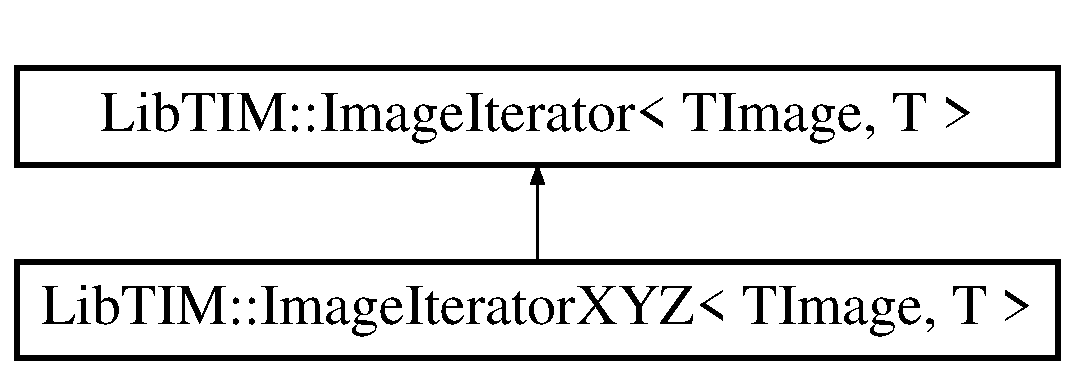
\includegraphics[height=2cm]{classLibTIM_1_1ImageIteratorXYZ}
\end{center}
\end{figure}
\subsection*{Public Member Functions}
\begin{CompactItemize}
\item 
{\bf Image\-Iterator\-XYZ} ()
\item 
{\bf Image\-Iterator\-XYZ} (T $\ast${\bf x})
\item 
void {\bf operator=} (const {\bf Image\-Iterator}$<$ TImage, T $>$ \&other)
\item 
{\bf Image\-Iterator\-XYZ} (const {\bf Image\-Iterator}$<$ TImage, T $>$ \&other)
\item 
T \& {\bf operator $\ast$} ()
\item 
T $\ast$ {\bf operator $\rightarrow$ } ()
\item 
{\bf Image\-Iterator\-XYZ}$<$ TImage, T $>$ \& {\bf operator++} ()
\item 
{\bf Image\-Iterator\-XYZ}$<$ TImage, T $>$ {\bf operator++} (int)
\end{CompactItemize}
\subsection*{Public Attributes}
\begin{CompactItemize}
\item 
{\bf TCoord} {\bf x}
\item 
{\bf TCoord} {\bf y}
\item 
{\bf TCoord} {\bf z}
\end{CompactItemize}
\subsubsection*{template$<$class TImage, class T$>$ class Lib\-TIM::Image\-Iterator\-XYZ$<$ TImage, T $>$}



\subsection{Constructor \& Destructor Documentation}
\index{LibTIM::ImageIteratorXYZ@{Lib\-TIM::Image\-Iterator\-XYZ}!ImageIteratorXYZ@{ImageIteratorXYZ}}
\index{ImageIteratorXYZ@{ImageIteratorXYZ}!LibTIM::ImageIteratorXYZ@{Lib\-TIM::Image\-Iterator\-XYZ}}
\subsubsection{\setlength{\rightskip}{0pt plus 5cm}template$<$class TImage, class T$>$ {\bf Lib\-TIM::Image\-Iterator\-XYZ}$<$ TImage, T $>$::{\bf Image\-Iterator\-XYZ} ()\hspace{0.3cm}{\tt  [inline]}}\label{classLibTIM_1_1ImageIteratorXYZ_a0}


\index{LibTIM::ImageIteratorXYZ@{Lib\-TIM::Image\-Iterator\-XYZ}!ImageIteratorXYZ@{ImageIteratorXYZ}}
\index{ImageIteratorXYZ@{ImageIteratorXYZ}!LibTIM::ImageIteratorXYZ@{Lib\-TIM::Image\-Iterator\-XYZ}}
\subsubsection{\setlength{\rightskip}{0pt plus 5cm}template$<$class TImage, class T$>$ {\bf Lib\-TIM::Image\-Iterator\-XYZ}$<$ TImage, T $>$::{\bf Image\-Iterator\-XYZ} (T $\ast$ {\em x})\hspace{0.3cm}{\tt  [inline]}}\label{classLibTIM_1_1ImageIteratorXYZ_a1}


\index{LibTIM::ImageIteratorXYZ@{Lib\-TIM::Image\-Iterator\-XYZ}!ImageIteratorXYZ@{ImageIteratorXYZ}}
\index{ImageIteratorXYZ@{ImageIteratorXYZ}!LibTIM::ImageIteratorXYZ@{Lib\-TIM::Image\-Iterator\-XYZ}}
\subsubsection{\setlength{\rightskip}{0pt plus 5cm}template$<$class TImage, class T$>$ {\bf Lib\-TIM::Image\-Iterator\-XYZ}$<$ TImage, T $>$::{\bf Image\-Iterator\-XYZ} (const {\bf Image\-Iterator}$<$ TImage, T $>$ \& {\em other})\hspace{0.3cm}{\tt  [inline]}}\label{classLibTIM_1_1ImageIteratorXYZ_a3}




\subsection{Member Function Documentation}
\index{LibTIM::ImageIteratorXYZ@{Lib\-TIM::Image\-Iterator\-XYZ}!operator *@{operator $\ast$}}
\index{operator *@{operator $\ast$}!LibTIM::ImageIteratorXYZ@{Lib\-TIM::Image\-Iterator\-XYZ}}
\subsubsection{\setlength{\rightskip}{0pt plus 5cm}template$<$class TImage, class T$>$ T\& {\bf Lib\-TIM::Image\-Iterator\-XYZ}$<$ TImage, T $>$::operator $\ast$ ()\hspace{0.3cm}{\tt  [inline]}}\label{classLibTIM_1_1ImageIteratorXYZ_a4}




Reimplemented from {\bf Lib\-TIM::Image\-Iterator$<$ TImage, T $>$} {\rm (p.\,\pageref{classLibTIM_1_1ImageIterator_a2})}.\index{LibTIM::ImageIteratorXYZ@{Lib\-TIM::Image\-Iterator\-XYZ}!operator++@{operator++}}
\index{operator++@{operator++}!LibTIM::ImageIteratorXYZ@{Lib\-TIM::Image\-Iterator\-XYZ}}
\subsubsection{\setlength{\rightskip}{0pt plus 5cm}template$<$class TImage, class T$>$ {\bf Image\-Iterator\-XYZ}$<$TImage, T$>$ {\bf Lib\-TIM::Image\-Iterator\-XYZ}$<$ TImage, T $>$::operator++ (int)\hspace{0.3cm}{\tt  [inline]}}\label{classLibTIM_1_1ImageIteratorXYZ_a7}




Reimplemented from {\bf Lib\-TIM::Image\-Iterator$<$ TImage, T $>$} {\rm (p.\,\pageref{classLibTIM_1_1ImageIterator_a5})}.\index{LibTIM::ImageIteratorXYZ@{Lib\-TIM::Image\-Iterator\-XYZ}!operator++@{operator++}}
\index{operator++@{operator++}!LibTIM::ImageIteratorXYZ@{Lib\-TIM::Image\-Iterator\-XYZ}}
\subsubsection{\setlength{\rightskip}{0pt plus 5cm}template$<$class TImage, class T$>$ {\bf Image\-Iterator\-XYZ}$<$TImage, T$>$\& {\bf Lib\-TIM::Image\-Iterator\-XYZ}$<$ TImage, T $>$::operator++ ()\hspace{0.3cm}{\tt  [inline]}}\label{classLibTIM_1_1ImageIteratorXYZ_a6}




Reimplemented from {\bf Lib\-TIM::Image\-Iterator$<$ TImage, T $>$} {\rm (p.\,\pageref{classLibTIM_1_1ImageIterator_a4})}.\index{LibTIM::ImageIteratorXYZ@{Lib\-TIM::Image\-Iterator\-XYZ}!operator->@{operator-$>$}}
\index{operator->@{operator-$>$}!LibTIM::ImageIteratorXYZ@{Lib\-TIM::Image\-Iterator\-XYZ}}
\subsubsection{\setlength{\rightskip}{0pt plus 5cm}template$<$class TImage, class T$>$ T$\ast$ {\bf Lib\-TIM::Image\-Iterator\-XYZ}$<$ TImage, T $>$::operator $\rightarrow$  ()\hspace{0.3cm}{\tt  [inline]}}\label{classLibTIM_1_1ImageIteratorXYZ_a5}




Reimplemented from {\bf Lib\-TIM::Image\-Iterator$<$ TImage, T $>$} {\rm (p.\,\pageref{classLibTIM_1_1ImageIterator_a3})}.\index{LibTIM::ImageIteratorXYZ@{Lib\-TIM::Image\-Iterator\-XYZ}!operator=@{operator=}}
\index{operator=@{operator=}!LibTIM::ImageIteratorXYZ@{Lib\-TIM::Image\-Iterator\-XYZ}}
\subsubsection{\setlength{\rightskip}{0pt plus 5cm}template$<$class TImage, class T$>$ void {\bf Lib\-TIM::Image\-Iterator\-XYZ}$<$ TImage, T $>$::operator= (const {\bf Image\-Iterator}$<$ TImage, T $>$ \& {\em other})\hspace{0.3cm}{\tt  [inline]}}\label{classLibTIM_1_1ImageIteratorXYZ_a2}




\subsection{Member Data Documentation}
\index{LibTIM::ImageIteratorXYZ@{Lib\-TIM::Image\-Iterator\-XYZ}!x@{x}}
\index{x@{x}!LibTIM::ImageIteratorXYZ@{Lib\-TIM::Image\-Iterator\-XYZ}}
\subsubsection{\setlength{\rightskip}{0pt plus 5cm}template$<$class TImage, class T$>$ {\bf TCoord} {\bf Lib\-TIM::Image\-Iterator\-XYZ}$<$ TImage, T $>$::{\bf x}}\label{classLibTIM_1_1ImageIteratorXYZ_o0}


\index{LibTIM::ImageIteratorXYZ@{Lib\-TIM::Image\-Iterator\-XYZ}!y@{y}}
\index{y@{y}!LibTIM::ImageIteratorXYZ@{Lib\-TIM::Image\-Iterator\-XYZ}}
\subsubsection{\setlength{\rightskip}{0pt plus 5cm}template$<$class TImage, class T$>$ {\bf TCoord} {\bf Lib\-TIM::Image\-Iterator\-XYZ}$<$ TImage, T $>$::{\bf y}}\label{classLibTIM_1_1ImageIteratorXYZ_o1}


\index{LibTIM::ImageIteratorXYZ@{Lib\-TIM::Image\-Iterator\-XYZ}!z@{z}}
\index{z@{z}!LibTIM::ImageIteratorXYZ@{Lib\-TIM::Image\-Iterator\-XYZ}}
\subsubsection{\setlength{\rightskip}{0pt plus 5cm}template$<$class TImage, class T$>$ {\bf TCoord} {\bf Lib\-TIM::Image\-Iterator\-XYZ}$<$ TImage, T $>$::{\bf z}}\label{classLibTIM_1_1ImageIteratorXYZ_o2}




The documentation for this class was generated from the following file:\begin{CompactItemize}
\item 
Common/{\bf Image\-Iterators.h}\end{CompactItemize}

\section{Lib\-TIM::Image\-Regions\-Infos$<$ T, T2 $>$ Class Template Reference}
\label{classLibTIM_1_1ImageRegionsInfos}\index{LibTIM::ImageRegionsInfos@{LibTIM::ImageRegionsInfos}}
{\tt \#include $<$Region\-Growing.h$>$}

\subsection*{Public Member Functions}
\begin{CompactItemize}
\item 
{\bf Image\-Regions\-Infos} ({\bf Image}$<$ T $>$ \&img, {\bf Image}$<$ T2 $>$ \&seed\-Regions)
\item 
double {\bf compute\-Distance} ({\bf Point}$<$ {\bf TCoord} $>$ \&p, {\bf Point}$<$ {\bf TCoord} $>$ \&q)
\begin{CompactList}\small\item\em Return the distance between p and q. The return value can be interpreted as a priority. \item\end{CompactList}\item 
double {\bf compute\-Distance} ({\bf TOffset} \&p, {\bf TOffset} \&q)
\item 
void {\bf set\-Point} ({\bf Point}$<$ {\bf TCoord} $>$ \&p, T2 label)
\item 
void {\bf set\-Point} ({\bf TOffset} \&p, T2 label)
\item 
void {\bf distance} ({\bf Point}$<$ {\bf TCoord} $>$ \&p, {\bf Point}$<$ {\bf TCoord} $>$ \&q)
\item 
void {\bf fusion} ({\bf Point}$<$ {\bf TCoord} $>$ \&p, T2 label)
\end{CompactItemize}
\subsubsection*{template$<$class T, class T2$>$ class Lib\-TIM::Image\-Regions\-Infos$<$ T, T2 $>$}



\subsection{Constructor \& Destructor Documentation}
\index{LibTIM::ImageRegionsInfos@{Lib\-TIM::Image\-Regions\-Infos}!ImageRegionsInfos@{ImageRegionsInfos}}
\index{ImageRegionsInfos@{ImageRegionsInfos}!LibTIM::ImageRegionsInfos@{Lib\-TIM::Image\-Regions\-Infos}}
\subsubsection{\setlength{\rightskip}{0pt plus 5cm}template$<$class T, class T2$>$ {\bf Lib\-TIM::Image\-Regions\-Infos}$<$ T, T2 $>$::{\bf Image\-Regions\-Infos} ({\bf Image}$<$ T $>$ \& {\em img}, {\bf Image}$<$ T2 $>$ \& {\em seed\-Regions})\hspace{0.3cm}{\tt  [inline]}}\label{classLibTIM_1_1ImageRegionsInfos_a0}




\subsection{Member Function Documentation}
\index{LibTIM::ImageRegionsInfos@{Lib\-TIM::Image\-Regions\-Infos}!computeDistance@{computeDistance}}
\index{computeDistance@{computeDistance}!LibTIM::ImageRegionsInfos@{Lib\-TIM::Image\-Regions\-Infos}}
\subsubsection{\setlength{\rightskip}{0pt plus 5cm}template$<$class T, class T2$>$ double {\bf Lib\-TIM::Image\-Regions\-Infos}$<$ T, T2 $>$::compute\-Distance ({\bf TOffset} \& {\em p}, {\bf TOffset} \& {\em q})\hspace{0.3cm}{\tt  [inline]}}\label{classLibTIM_1_1ImageRegionsInfos_a2}


\index{LibTIM::ImageRegionsInfos@{Lib\-TIM::Image\-Regions\-Infos}!computeDistance@{computeDistance}}
\index{computeDistance@{computeDistance}!LibTIM::ImageRegionsInfos@{Lib\-TIM::Image\-Regions\-Infos}}
\subsubsection{\setlength{\rightskip}{0pt plus 5cm}template$<$class T, class T2$>$ double {\bf Lib\-TIM::Image\-Regions\-Infos}$<$ T, T2 $>$::compute\-Distance ({\bf Point}$<$ {\bf TCoord} $>$ \& {\em p}, {\bf Point}$<$ {\bf TCoord} $>$ \& {\em q})\hspace{0.3cm}{\tt  [inline]}}\label{classLibTIM_1_1ImageRegionsInfos_a1}


Return the distance between p and q. The return value can be interpreted as a priority. 

\index{LibTIM::ImageRegionsInfos@{Lib\-TIM::Image\-Regions\-Infos}!distance@{distance}}
\index{distance@{distance}!LibTIM::ImageRegionsInfos@{Lib\-TIM::Image\-Regions\-Infos}}
\subsubsection{\setlength{\rightskip}{0pt plus 5cm}template$<$class T, class T2$>$ void {\bf Lib\-TIM::Image\-Regions\-Infos}$<$ T, T2 $>$::distance ({\bf Point}$<$ {\bf TCoord} $>$ \& {\em p}, {\bf Point}$<$ {\bf TCoord} $>$ \& {\em q})\hspace{0.3cm}{\tt  [inline]}}\label{classLibTIM_1_1ImageRegionsInfos_a5}


\index{LibTIM::ImageRegionsInfos@{Lib\-TIM::Image\-Regions\-Infos}!fusion@{fusion}}
\index{fusion@{fusion}!LibTIM::ImageRegionsInfos@{Lib\-TIM::Image\-Regions\-Infos}}
\subsubsection{\setlength{\rightskip}{0pt plus 5cm}template$<$class T, class T2$>$ void {\bf Lib\-TIM::Image\-Regions\-Infos}$<$ T, T2 $>$::fusion ({\bf Point}$<$ {\bf TCoord} $>$ \& {\em p}, T2 {\em label})\hspace{0.3cm}{\tt  [inline]}}\label{classLibTIM_1_1ImageRegionsInfos_a6}


\index{LibTIM::ImageRegionsInfos@{Lib\-TIM::Image\-Regions\-Infos}!setPoint@{setPoint}}
\index{setPoint@{setPoint}!LibTIM::ImageRegionsInfos@{Lib\-TIM::Image\-Regions\-Infos}}
\subsubsection{\setlength{\rightskip}{0pt plus 5cm}template$<$class T, class T2$>$ void {\bf Lib\-TIM::Image\-Regions\-Infos}$<$ T, T2 $>$::set\-Point ({\bf TOffset} \& {\em p}, T2 {\em label})\hspace{0.3cm}{\tt  [inline]}}\label{classLibTIM_1_1ImageRegionsInfos_a4}


\index{LibTIM::ImageRegionsInfos@{Lib\-TIM::Image\-Regions\-Infos}!setPoint@{setPoint}}
\index{setPoint@{setPoint}!LibTIM::ImageRegionsInfos@{Lib\-TIM::Image\-Regions\-Infos}}
\subsubsection{\setlength{\rightskip}{0pt plus 5cm}template$<$class T, class T2$>$ void {\bf Lib\-TIM::Image\-Regions\-Infos}$<$ T, T2 $>$::set\-Point ({\bf Point}$<$ {\bf TCoord} $>$ \& {\em p}, T2 {\em label})\hspace{0.3cm}{\tt  [inline]}}\label{classLibTIM_1_1ImageRegionsInfos_a3}




The documentation for this class was generated from the following file:\begin{CompactItemize}
\item 
Algorithms/{\bf Region\-Growing.h}\end{CompactItemize}

\section{Lib\-TIM::Node Struct Reference}
\label{structLibTIM_1_1Node}\index{LibTIM::Node@{LibTIM::Node}}
{\tt \#include $<$Component\-Tree.hxx$>$}

\subsection*{Public Attributes}
\begin{CompactItemize}
\item 
int {\bf label}
\item 
int {\bf h}
\item 
int {\bf area}
\item 
{\bf Node} $\ast$ {\bf father}
\item 
std::vector$<$ long int $>$ {\bf pixels}
\item 
std::vector$<$ struct {\bf Node} $\ast$ $>$ {\bf childs}
\item 
bool {\bf active}
\end{CompactItemize}


\subsection{Member Data Documentation}
\index{LibTIM::Node@{Lib\-TIM::Node}!active@{active}}
\index{active@{active}!LibTIM::Node@{Lib\-TIM::Node}}
\subsubsection{\setlength{\rightskip}{0pt plus 5cm}bool {\bf Lib\-TIM::Node::active}}\label{structLibTIM_1_1Node_o6}


\index{LibTIM::Node@{Lib\-TIM::Node}!area@{area}}
\index{area@{area}!LibTIM::Node@{Lib\-TIM::Node}}
\subsubsection{\setlength{\rightskip}{0pt plus 5cm}int {\bf Lib\-TIM::Node::area}}\label{structLibTIM_1_1Node_o2}


\index{LibTIM::Node@{Lib\-TIM::Node}!childs@{childs}}
\index{childs@{childs}!LibTIM::Node@{Lib\-TIM::Node}}
\subsubsection{\setlength{\rightskip}{0pt plus 5cm}std::vector$<$struct {\bf Node} $\ast$$>$ {\bf Lib\-TIM::Node::childs}}\label{structLibTIM_1_1Node_o5}


\index{LibTIM::Node@{Lib\-TIM::Node}!father@{father}}
\index{father@{father}!LibTIM::Node@{Lib\-TIM::Node}}
\subsubsection{\setlength{\rightskip}{0pt plus 5cm}struct {\bf Node}$\ast$ {\bf Lib\-TIM::Node::father}}\label{structLibTIM_1_1Node_o3}


\index{LibTIM::Node@{Lib\-TIM::Node}!h@{h}}
\index{h@{h}!LibTIM::Node@{Lib\-TIM::Node}}
\subsubsection{\setlength{\rightskip}{0pt plus 5cm}int {\bf Lib\-TIM::Node::h}}\label{structLibTIM_1_1Node_o1}


\index{LibTIM::Node@{Lib\-TIM::Node}!label@{label}}
\index{label@{label}!LibTIM::Node@{Lib\-TIM::Node}}
\subsubsection{\setlength{\rightskip}{0pt plus 5cm}int {\bf Lib\-TIM::Node::label}}\label{structLibTIM_1_1Node_o0}


\index{LibTIM::Node@{Lib\-TIM::Node}!pixels@{pixels}}
\index{pixels@{pixels}!LibTIM::Node@{Lib\-TIM::Node}}
\subsubsection{\setlength{\rightskip}{0pt plus 5cm}std::vector$<$long int $>$ {\bf Lib\-TIM::Node::pixels}}\label{structLibTIM_1_1Node_o4}




The documentation for this struct was generated from the following file:\begin{CompactItemize}
\item 
Algorithms/{\bf Component\-Tree.hxx}\end{CompactItemize}

\section{Lib\-TIM::Non\-Flat\-SE$<$ T $>$ Class Template Reference}
\label{classLibTIM_1_1NonFlatSE}\index{LibTIM::NonFlatSE@{LibTIM::NonFlatSE}}
Non-flat structuring elements (or ponderated masks).  


{\tt \#include $<$Non\-Flat\-SE.h$>$}

Inheritance diagram for Lib\-TIM::Non\-Flat\-SE$<$ T $>$::\begin{figure}[H]
\begin{center}
\leavevmode
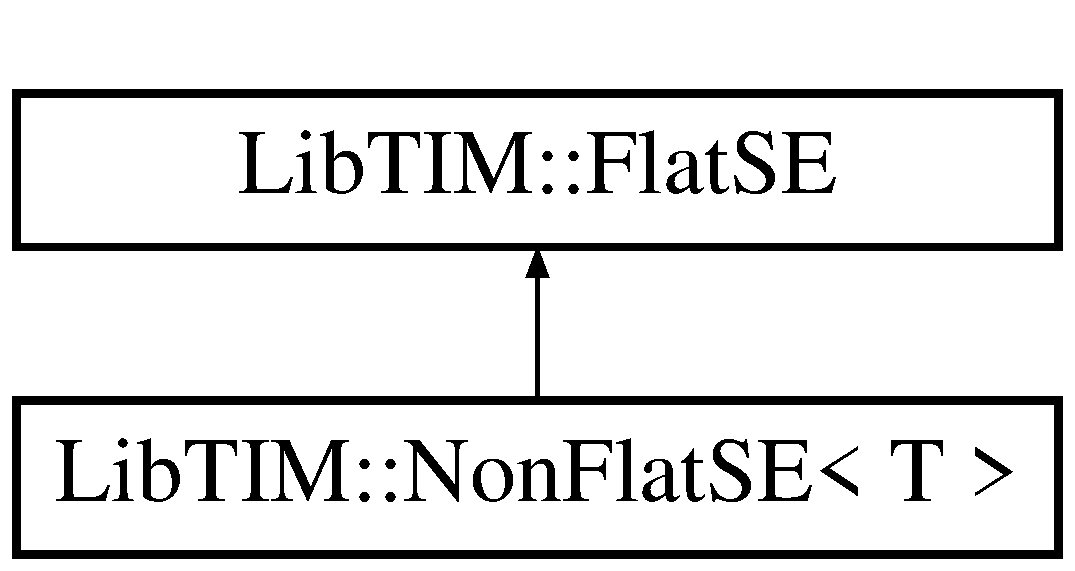
\includegraphics[height=2cm]{classLibTIM_1_1NonFlatSE}
\end{center}
\end{figure}
\subsection*{Public Member Functions}
\begin{CompactItemize}
\item 
{\bf Non\-Flat\-SE} ()
\item 
{\bf $\sim$Non\-Flat\-SE} ()
\item 
void {\bf make\-Chamfer2D} ()
\item 
{\bf Non\-Flat\-SE} {\bf raster\-Scan} ()
\item 
{\bf Non\-Flat\-SE} {\bf anti\-Raster\-Scan} ()
\item 
double {\bf get\-Norm} () const 
\item 
T {\bf get\-Value} (int i) const 
\item 
void {\bf add\-Point} ({\bf Point}$<$ {\bf TCoord} $>$ p, T attribute)
\item 
void {\bf print} ()
\item 
void {\bf reserve} (size\_\-t size)
\item 
void {\bf clear} ()
\item 
template$<$$>$ void {\bf make\-Chamfer2D} ()
\end{CompactItemize}


\subsection{Detailed Description}
\subsubsection*{template$<$class T$>$ class Lib\-TIM::Non\-Flat\-SE$<$ T $>$}

Non-flat structuring elements (or ponderated masks). 

Can be used for convolution, chanfrein masks, or non-flat morphology



\subsection{Constructor \& Destructor Documentation}
\index{LibTIM::NonFlatSE@{Lib\-TIM::Non\-Flat\-SE}!NonFlatSE@{NonFlatSE}}
\index{NonFlatSE@{NonFlatSE}!LibTIM::NonFlatSE@{Lib\-TIM::Non\-Flat\-SE}}
\subsubsection{\setlength{\rightskip}{0pt plus 5cm}template$<$class T$>$ {\bf Lib\-TIM::Non\-Flat\-SE}$<$ T $>$::{\bf Non\-Flat\-SE} ()\hspace{0.3cm}{\tt  [inline]}}\label{classLibTIM_1_1NonFlatSE_a0}


\index{LibTIM::NonFlatSE@{Lib\-TIM::Non\-Flat\-SE}!~NonFlatSE@{$\sim$NonFlatSE}}
\index{~NonFlatSE@{$\sim$NonFlatSE}!LibTIM::NonFlatSE@{Lib\-TIM::Non\-Flat\-SE}}
\subsubsection{\setlength{\rightskip}{0pt plus 5cm}template$<$class T$>$ {\bf Lib\-TIM::Non\-Flat\-SE}$<$ T $>$::$\sim${\bf Non\-Flat\-SE} ()\hspace{0.3cm}{\tt  [inline]}}\label{classLibTIM_1_1NonFlatSE_a1}




\subsection{Member Function Documentation}
\index{LibTIM::NonFlatSE@{Lib\-TIM::Non\-Flat\-SE}!addPoint@{addPoint}}
\index{addPoint@{addPoint}!LibTIM::NonFlatSE@{Lib\-TIM::Non\-Flat\-SE}}
\subsubsection{\setlength{\rightskip}{0pt plus 5cm}template$<$class T$>$ void {\bf Lib\-TIM::Non\-Flat\-SE}$<$ T $>$::add\-Point ({\bf Point}$<$ {\bf TCoord} $>$ {\em p}, T {\em attribute})\hspace{0.3cm}{\tt  [inline]}}\label{classLibTIM_1_1NonFlatSE_a7}


\index{LibTIM::NonFlatSE@{Lib\-TIM::Non\-Flat\-SE}!antiRasterScan@{antiRasterScan}}
\index{antiRasterScan@{antiRasterScan}!LibTIM::NonFlatSE@{Lib\-TIM::Non\-Flat\-SE}}
\subsubsection{\setlength{\rightskip}{0pt plus 5cm}template$<$class T$>$ {\bf Non\-Flat\-SE}$<$ T $>$ {\bf Lib\-TIM::Non\-Flat\-SE}$<$ T $>$::anti\-Raster\-Scan ()}\label{classLibTIM_1_1NonFlatSE_a4}


\index{LibTIM::NonFlatSE@{Lib\-TIM::Non\-Flat\-SE}!clear@{clear}}
\index{clear@{clear}!LibTIM::NonFlatSE@{Lib\-TIM::Non\-Flat\-SE}}
\subsubsection{\setlength{\rightskip}{0pt plus 5cm}template$<$class T$>$ void {\bf Lib\-TIM::Non\-Flat\-SE}$<$ T $>$::clear ()\hspace{0.3cm}{\tt  [inline]}}\label{classLibTIM_1_1NonFlatSE_a10}




Reimplemented from {\bf Lib\-TIM::Flat\-SE} {\rm (p.\,\pageref{classLibTIM_1_1FlatSE_a30})}.\index{LibTIM::NonFlatSE@{Lib\-TIM::Non\-Flat\-SE}!getNorm@{getNorm}}
\index{getNorm@{getNorm}!LibTIM::NonFlatSE@{Lib\-TIM::Non\-Flat\-SE}}
\subsubsection{\setlength{\rightskip}{0pt plus 5cm}template$<$class T$>$ double {\bf Lib\-TIM::Non\-Flat\-SE}$<$ T $>$::get\-Norm () const}\label{classLibTIM_1_1NonFlatSE_a5}


\index{LibTIM::NonFlatSE@{Lib\-TIM::Non\-Flat\-SE}!getValue@{getValue}}
\index{getValue@{getValue}!LibTIM::NonFlatSE@{Lib\-TIM::Non\-Flat\-SE}}
\subsubsection{\setlength{\rightskip}{0pt plus 5cm}template$<$class T$>$ T {\bf Lib\-TIM::Non\-Flat\-SE}$<$ T $>$::get\-Value (int {\em i}) const\hspace{0.3cm}{\tt  [inline]}}\label{classLibTIM_1_1NonFlatSE_a6}


\index{LibTIM::NonFlatSE@{Lib\-TIM::Non\-Flat\-SE}!makeChamfer2D@{makeChamfer2D}}
\index{makeChamfer2D@{makeChamfer2D}!LibTIM::NonFlatSE@{Lib\-TIM::Non\-Flat\-SE}}
\subsubsection{\setlength{\rightskip}{0pt plus 5cm}template$<$$>$ void {\bf Lib\-TIM::Non\-Flat\-SE}$<$ {\bf U8} $>$::make\-Chamfer2D ()\hspace{0.3cm}{\tt  [inline]}}\label{classLibTIM_1_1NonFlatSE_a11}


\index{LibTIM::NonFlatSE@{Lib\-TIM::Non\-Flat\-SE}!makeChamfer2D@{makeChamfer2D}}
\index{makeChamfer2D@{makeChamfer2D}!LibTIM::NonFlatSE@{Lib\-TIM::Non\-Flat\-SE}}
\subsubsection{\setlength{\rightskip}{0pt plus 5cm}template$<$class T$>$ void {\bf Lib\-TIM::Non\-Flat\-SE}$<$ T $>$::make\-Chamfer2D ()}\label{classLibTIM_1_1NonFlatSE_a2}


\index{LibTIM::NonFlatSE@{Lib\-TIM::Non\-Flat\-SE}!print@{print}}
\index{print@{print}!LibTIM::NonFlatSE@{Lib\-TIM::Non\-Flat\-SE}}
\subsubsection{\setlength{\rightskip}{0pt plus 5cm}template$<$class T$>$ void {\bf Lib\-TIM::Non\-Flat\-SE}$<$ T $>$::print ()\hspace{0.3cm}{\tt  [inline]}}\label{classLibTIM_1_1NonFlatSE_a8}




Reimplemented from {\bf Lib\-TIM::Flat\-SE} {\rm (p.\,\pageref{classLibTIM_1_1FlatSE_a28})}.\index{LibTIM::NonFlatSE@{Lib\-TIM::Non\-Flat\-SE}!rasterScan@{rasterScan}}
\index{rasterScan@{rasterScan}!LibTIM::NonFlatSE@{Lib\-TIM::Non\-Flat\-SE}}
\subsubsection{\setlength{\rightskip}{0pt plus 5cm}template$<$class T$>$ {\bf Non\-Flat\-SE}$<$ T $>$ {\bf Lib\-TIM::Non\-Flat\-SE}$<$ T $>$::raster\-Scan ()}\label{classLibTIM_1_1NonFlatSE_a3}


\index{LibTIM::NonFlatSE@{Lib\-TIM::Non\-Flat\-SE}!reserve@{reserve}}
\index{reserve@{reserve}!LibTIM::NonFlatSE@{Lib\-TIM::Non\-Flat\-SE}}
\subsubsection{\setlength{\rightskip}{0pt plus 5cm}template$<$class T$>$ void {\bf Lib\-TIM::Non\-Flat\-SE}$<$ T $>$::reserve (size\_\-t {\em size})\hspace{0.3cm}{\tt  [inline]}}\label{classLibTIM_1_1NonFlatSE_a9}




Reimplemented from {\bf Lib\-TIM::Flat\-SE} {\rm (p.\,\pageref{classLibTIM_1_1FlatSE_a29})}.

The documentation for this class was generated from the following files:\begin{CompactItemize}
\item 
Common/{\bf Non\-Flat\-SE.h}\item 
Common/{\bf Non\-Flat\-SE.hxx}\end{CompactItemize}

\section{Lib\-TIM::Ordered\-Queue$<$ T $>$ Class Template Reference}
\label{classLibTIM_1_1OrderedQueue}\index{LibTIM::OrderedQueue@{LibTIM::OrderedQueue}}
Ordered {\bf Queue}{\rm (p.\,\pageref{classLibTIM_1_1Queue})}.  


{\tt \#include $<$Ordered\-Queue.h$>$}

\subsection*{Public Member Functions}
\begin{CompactItemize}
\item 
{\bf Ordered\-Queue} ()
\begin{CompactList}\small\item\em Creates an empty ordered queue. \item\end{CompactList}\item 
{\bf $\sim$Ordered\-Queue} ()
\item 
void {\bf put} (int order, T \_\-val)
\begin{CompactList}\small\item\em add an element in OQ with specified order \item\end{CompactList}\item 
T {\bf get} ()
\begin{CompactList}\small\item\em get a element in OQueue \item\end{CompactList}\item 
bool {\bf empty} ()
\begin{CompactList}\small\item\em bool if OQueue is empty \item\end{CompactList}\end{CompactItemize}


\subsection{Detailed Description}
\subsubsection*{template$<$class T$>$ class Lib\-TIM::Ordered\-Queue$<$ T $>$}

Ordered {\bf Queue}{\rm (p.\,\pageref{classLibTIM_1_1Queue})}. 

This structure allow the use of ordered queue, it is templated to deal with any type. the order is integer and decreasing ( order=0 have more priority than order=1)



\subsection{Constructor \& Destructor Documentation}
\index{LibTIM::OrderedQueue@{Lib\-TIM::Ordered\-Queue}!OrderedQueue@{OrderedQueue}}
\index{OrderedQueue@{OrderedQueue}!LibTIM::OrderedQueue@{Lib\-TIM::Ordered\-Queue}}
\subsubsection{\setlength{\rightskip}{0pt plus 5cm}template$<$class T$>$ {\bf Lib\-TIM::Ordered\-Queue}$<$ T $>$::{\bf Ordered\-Queue} ()\hspace{0.3cm}{\tt  [inline]}}\label{classLibTIM_1_1OrderedQueue_a0}


Creates an empty ordered queue. 

\index{LibTIM::OrderedQueue@{Lib\-TIM::Ordered\-Queue}!~OrderedQueue@{$\sim$OrderedQueue}}
\index{~OrderedQueue@{$\sim$OrderedQueue}!LibTIM::OrderedQueue@{Lib\-TIM::Ordered\-Queue}}
\subsubsection{\setlength{\rightskip}{0pt plus 5cm}template$<$class T$>$ {\bf Lib\-TIM::Ordered\-Queue}$<$ T $>$::$\sim${\bf Ordered\-Queue} ()\hspace{0.3cm}{\tt  [inline]}}\label{classLibTIM_1_1OrderedQueue_a1}




\subsection{Member Function Documentation}
\index{LibTIM::OrderedQueue@{Lib\-TIM::Ordered\-Queue}!empty@{empty}}
\index{empty@{empty}!LibTIM::OrderedQueue@{Lib\-TIM::Ordered\-Queue}}
\subsubsection{\setlength{\rightskip}{0pt plus 5cm}template$<$class T$>$ bool {\bf Lib\-TIM::Ordered\-Queue}$<$ T $>$::empty ()\hspace{0.3cm}{\tt  [inline]}}\label{classLibTIM_1_1OrderedQueue_a4}


bool if OQueue is empty 

\index{LibTIM::OrderedQueue@{Lib\-TIM::Ordered\-Queue}!get@{get}}
\index{get@{get}!LibTIM::OrderedQueue@{Lib\-TIM::Ordered\-Queue}}
\subsubsection{\setlength{\rightskip}{0pt plus 5cm}template$<$class T$>$ T {\bf Lib\-TIM::Ordered\-Queue}$<$ T $>$::get ()\hspace{0.3cm}{\tt  [inline]}}\label{classLibTIM_1_1OrderedQueue_a3}


get a element in OQueue 

\index{LibTIM::OrderedQueue@{Lib\-TIM::Ordered\-Queue}!put@{put}}
\index{put@{put}!LibTIM::OrderedQueue@{Lib\-TIM::Ordered\-Queue}}
\subsubsection{\setlength{\rightskip}{0pt plus 5cm}template$<$class T$>$ void {\bf Lib\-TIM::Ordered\-Queue}$<$ T $>$::put (int {\em order}, T {\em \_\-val})\hspace{0.3cm}{\tt  [inline]}}\label{classLibTIM_1_1OrderedQueue_a2}


add an element in OQ with specified order 



The documentation for this class was generated from the following file:\begin{CompactItemize}
\item 
Common/{\bf Ordered\-Queue.h}\end{CompactItemize}

\section{Lib\-TIM::Ordered\-Queue\-Double$<$ T $>$ Class Template Reference}
\label{classLibTIM_1_1OrderedQueueDouble}\index{LibTIM::OrderedQueueDouble@{LibTIM::OrderedQueueDouble}}
Ordered {\bf Queue}{\rm (p.\,\pageref{classLibTIM_1_1Queue})} with double priority.  


{\tt \#include $<$Ordered\-Queue.h$>$}

\subsection*{Public Member Functions}
\begin{CompactItemize}
\item 
{\bf Ordered\-Queue\-Double} ()
\begin{CompactList}\small\item\em Creates an empty ordered queue. \item\end{CompactList}\item 
{\bf $\sim$Ordered\-Queue\-Double} ()
\item 
void {\bf put} (double order, T \_\-val)
\begin{CompactList}\small\item\em add an element in OQ with specified order \item\end{CompactList}\item 
T {\bf get} ()
\begin{CompactList}\small\item\em get a element in OQueue \item\end{CompactList}\item 
bool {\bf empty} ()
\begin{CompactList}\small\item\em bool if OQueue is empty \item\end{CompactList}\end{CompactItemize}


\subsection{Detailed Description}
\subsubsection*{template$<$class T$>$ class Lib\-TIM::Ordered\-Queue\-Double$<$ T $>$}

Ordered {\bf Queue}{\rm (p.\,\pageref{classLibTIM_1_1Queue})} with double priority. 

This structure allow the use of ordered queue, it is templated to deal with any type. the order is double and is decreasing ( order=0 have more priority than order=1)



\subsection{Constructor \& Destructor Documentation}
\index{LibTIM::OrderedQueueDouble@{Lib\-TIM::Ordered\-Queue\-Double}!OrderedQueueDouble@{OrderedQueueDouble}}
\index{OrderedQueueDouble@{OrderedQueueDouble}!LibTIM::OrderedQueueDouble@{Lib\-TIM::Ordered\-Queue\-Double}}
\subsubsection{\setlength{\rightskip}{0pt plus 5cm}template$<$class T$>$ {\bf Lib\-TIM::Ordered\-Queue\-Double}$<$ T $>$::{\bf Ordered\-Queue\-Double} ()\hspace{0.3cm}{\tt  [inline]}}\label{classLibTIM_1_1OrderedQueueDouble_a0}


Creates an empty ordered queue. 

\index{LibTIM::OrderedQueueDouble@{Lib\-TIM::Ordered\-Queue\-Double}!~OrderedQueueDouble@{$\sim$OrderedQueueDouble}}
\index{~OrderedQueueDouble@{$\sim$OrderedQueueDouble}!LibTIM::OrderedQueueDouble@{Lib\-TIM::Ordered\-Queue\-Double}}
\subsubsection{\setlength{\rightskip}{0pt plus 5cm}template$<$class T$>$ {\bf Lib\-TIM::Ordered\-Queue\-Double}$<$ T $>$::$\sim${\bf Ordered\-Queue\-Double} ()\hspace{0.3cm}{\tt  [inline]}}\label{classLibTIM_1_1OrderedQueueDouble_a1}




\subsection{Member Function Documentation}
\index{LibTIM::OrderedQueueDouble@{Lib\-TIM::Ordered\-Queue\-Double}!empty@{empty}}
\index{empty@{empty}!LibTIM::OrderedQueueDouble@{Lib\-TIM::Ordered\-Queue\-Double}}
\subsubsection{\setlength{\rightskip}{0pt plus 5cm}template$<$class T$>$ bool {\bf Lib\-TIM::Ordered\-Queue\-Double}$<$ T $>$::empty ()\hspace{0.3cm}{\tt  [inline]}}\label{classLibTIM_1_1OrderedQueueDouble_a4}


bool if OQueue is empty 

\index{LibTIM::OrderedQueueDouble@{Lib\-TIM::Ordered\-Queue\-Double}!get@{get}}
\index{get@{get}!LibTIM::OrderedQueueDouble@{Lib\-TIM::Ordered\-Queue\-Double}}
\subsubsection{\setlength{\rightskip}{0pt plus 5cm}template$<$class T$>$ T {\bf Lib\-TIM::Ordered\-Queue\-Double}$<$ T $>$::get ()\hspace{0.3cm}{\tt  [inline]}}\label{classLibTIM_1_1OrderedQueueDouble_a3}


get a element in OQueue 

\index{LibTIM::OrderedQueueDouble@{Lib\-TIM::Ordered\-Queue\-Double}!put@{put}}
\index{put@{put}!LibTIM::OrderedQueueDouble@{Lib\-TIM::Ordered\-Queue\-Double}}
\subsubsection{\setlength{\rightskip}{0pt plus 5cm}template$<$class T$>$ void {\bf Lib\-TIM::Ordered\-Queue\-Double}$<$ T $>$::put (double {\em order}, T {\em \_\-val})\hspace{0.3cm}{\tt  [inline]}}\label{classLibTIM_1_1OrderedQueueDouble_a2}


add an element in OQ with specified order 



The documentation for this class was generated from the following file:\begin{CompactItemize}
\item 
Common/{\bf Ordered\-Queue.h}\end{CompactItemize}

\section{Lib\-TIM::Point$<$ T $>$ Class Template Reference}
\label{classLibTIM_1_1Point}\index{LibTIM::Point@{LibTIM::Point}}
{\bf Point}{\rm (p.\,\pageref{classLibTIM_1_1Point})} Structure.  


{\tt \#include $<$Point.h$>$}

\subsection*{Public Member Functions}
\begin{CompactItemize}
\item 
{\bf Point} ({\bf TCoord} {\bf x}=0, {\bf TCoord} {\bf y}=0, {\bf TCoord} {\bf z}=0)
\item 
{\bf Point} \& {\bf operator+=} ({\bf Point}$<$ T $>$ q)
\item 
{\bf Point} \& {\bf operator-=} ({\bf Point}$<$ T $>$ q)
\item 
bool {\bf operator==} ({\bf Point}$<$ T $>$ q)
\item 
void {\bf operator=} (const {\bf Point}$<$ T $>$ \&q)
\item 
{\bf Point} (const {\bf Point} \&q)
\item 
void {\bf operator()} (T {\bf x}, T {\bf y}, T {\bf z})
\item 
void {\bf print} ()
\end{CompactItemize}
\subsection*{Public Attributes}
\begin{CompactItemize}
\item 
T {\bf x}
\item 
T {\bf y}
\item 
T {\bf z}
\end{CompactItemize}


\subsection{Detailed Description}
\subsubsection*{template$<$class T$>$ class Lib\-TIM::Point$<$ T $>$}

{\bf Point}{\rm (p.\,\pageref{classLibTIM_1_1Point})} Structure. 

Basic structure to manipulate 3D points of type T



\subsection{Constructor \& Destructor Documentation}
\index{LibTIM::Point@{Lib\-TIM::Point}!Point@{Point}}
\index{Point@{Point}!LibTIM::Point@{Lib\-TIM::Point}}
\subsubsection{\setlength{\rightskip}{0pt plus 5cm}template$<$class T$>$ {\bf Lib\-TIM::Point}$<$ T $>$::{\bf Point} ({\bf TCoord} {\em x} = {\tt 0}, {\bf TCoord} {\em y} = {\tt 0}, {\bf TCoord} {\em z} = {\tt 0})\hspace{0.3cm}{\tt  [inline]}}\label{classLibTIM_1_1Point_a0}


\index{LibTIM::Point@{Lib\-TIM::Point}!Point@{Point}}
\index{Point@{Point}!LibTIM::Point@{Lib\-TIM::Point}}
\subsubsection{\setlength{\rightskip}{0pt plus 5cm}template$<$class T$>$ {\bf Lib\-TIM::Point}$<$ T $>$::{\bf Point} (const {\bf Point}$<$ T $>$ \& {\em q})\hspace{0.3cm}{\tt  [inline]}}\label{classLibTIM_1_1Point_a5}




\subsection{Member Function Documentation}
\index{LibTIM::Point@{Lib\-TIM::Point}!operator()@{operator()}}
\index{operator()@{operator()}!LibTIM::Point@{Lib\-TIM::Point}}
\subsubsection{\setlength{\rightskip}{0pt plus 5cm}template$<$class T$>$ void {\bf Lib\-TIM::Point}$<$ T $>$::operator() (T {\em x}, T {\em y}, T {\em z})\hspace{0.3cm}{\tt  [inline]}}\label{classLibTIM_1_1Point_a6}


\index{LibTIM::Point@{Lib\-TIM::Point}!operator+=@{operator+=}}
\index{operator+=@{operator+=}!LibTIM::Point@{Lib\-TIM::Point}}
\subsubsection{\setlength{\rightskip}{0pt plus 5cm}template$<$class T$>$ {\bf Point}\& {\bf Lib\-TIM::Point}$<$ T $>$::operator+= ({\bf Point}$<$ T $>$ {\em q})\hspace{0.3cm}{\tt  [inline]}}\label{classLibTIM_1_1Point_a1}


\index{LibTIM::Point@{Lib\-TIM::Point}!operator-=@{operator-=}}
\index{operator-=@{operator-=}!LibTIM::Point@{Lib\-TIM::Point}}
\subsubsection{\setlength{\rightskip}{0pt plus 5cm}template$<$class T$>$ {\bf Point}\& {\bf Lib\-TIM::Point}$<$ T $>$::operator-= ({\bf Point}$<$ T $>$ {\em q})\hspace{0.3cm}{\tt  [inline]}}\label{classLibTIM_1_1Point_a2}


\index{LibTIM::Point@{Lib\-TIM::Point}!operator=@{operator=}}
\index{operator=@{operator=}!LibTIM::Point@{Lib\-TIM::Point}}
\subsubsection{\setlength{\rightskip}{0pt plus 5cm}template$<$class T$>$ void {\bf Lib\-TIM::Point}$<$ T $>$::operator= (const {\bf Point}$<$ T $>$ \& {\em q})\hspace{0.3cm}{\tt  [inline]}}\label{classLibTIM_1_1Point_a4}


\index{LibTIM::Point@{Lib\-TIM::Point}!operator==@{operator==}}
\index{operator==@{operator==}!LibTIM::Point@{Lib\-TIM::Point}}
\subsubsection{\setlength{\rightskip}{0pt plus 5cm}template$<$class T$>$ bool {\bf Lib\-TIM::Point}$<$ T $>$::operator== ({\bf Point}$<$ T $>$ {\em q})\hspace{0.3cm}{\tt  [inline]}}\label{classLibTIM_1_1Point_a3}


\index{LibTIM::Point@{Lib\-TIM::Point}!print@{print}}
\index{print@{print}!LibTIM::Point@{Lib\-TIM::Point}}
\subsubsection{\setlength{\rightskip}{0pt plus 5cm}template$<$class T$>$ void {\bf Lib\-TIM::Point}$<$ T $>$::print ()\hspace{0.3cm}{\tt  [inline]}}\label{classLibTIM_1_1Point_a7}




\subsection{Member Data Documentation}
\index{LibTIM::Point@{Lib\-TIM::Point}!x@{x}}
\index{x@{x}!LibTIM::Point@{Lib\-TIM::Point}}
\subsubsection{\setlength{\rightskip}{0pt plus 5cm}template$<$class T$>$ T {\bf Lib\-TIM::Point}$<$ T $>$::{\bf x}}\label{classLibTIM_1_1Point_o0}


\index{LibTIM::Point@{Lib\-TIM::Point}!y@{y}}
\index{y@{y}!LibTIM::Point@{Lib\-TIM::Point}}
\subsubsection{\setlength{\rightskip}{0pt plus 5cm}template$<$class T$>$ T {\bf Lib\-TIM::Point}$<$ T $>$::{\bf y}}\label{classLibTIM_1_1Point_o1}


\index{LibTIM::Point@{Lib\-TIM::Point}!z@{z}}
\index{z@{z}!LibTIM::Point@{Lib\-TIM::Point}}
\subsubsection{\setlength{\rightskip}{0pt plus 5cm}template$<$class T$>$ T {\bf Lib\-TIM::Point}$<$ T $>$::{\bf z}}\label{classLibTIM_1_1Point_o2}




The documentation for this class was generated from the following file:\begin{CompactItemize}
\item 
Common/{\bf Point.h}\end{CompactItemize}

\section{Lib\-TIM::Queue$<$ T $>$ Class Template Reference}
\label{classLibTIM_1_1Queue}\index{LibTIM::Queue@{LibTIM::Queue}}
{\tt \#include $<$Ordered\-Queue.h$>$}

\subsection*{Public Member Functions}
\begin{CompactItemize}
\item 
{\bf Queue} ()
\item 
void {\bf put} (T \_\-t)
\begin{CompactList}\small\item\em add an element in {\bf Queue}{\rm (p.\,\pageref{classLibTIM_1_1Queue})} \item\end{CompactList}\item 
T {\bf get} ()
\begin{CompactList}\small\item\em get a element in {\bf Queue}{\rm (p.\,\pageref{classLibTIM_1_1Queue})} \item\end{CompactList}\item 
bool {\bf empty} ()
\begin{CompactList}\small\item\em bool if {\bf Queue}{\rm (p.\,\pageref{classLibTIM_1_1Queue})} is empty \item\end{CompactList}\end{CompactItemize}
\subsubsection*{template$<$class T$>$ class Lib\-TIM::Queue$<$ T $>$}



\subsection{Constructor \& Destructor Documentation}
\index{LibTIM::Queue@{Lib\-TIM::Queue}!Queue@{Queue}}
\index{Queue@{Queue}!LibTIM::Queue@{Lib\-TIM::Queue}}
\subsubsection{\setlength{\rightskip}{0pt plus 5cm}template$<$class T$>$ {\bf Lib\-TIM::Queue}$<$ T $>$::{\bf Queue} ()\hspace{0.3cm}{\tt  [inline]}}\label{classLibTIM_1_1Queue_a0}




\subsection{Member Function Documentation}
\index{LibTIM::Queue@{Lib\-TIM::Queue}!empty@{empty}}
\index{empty@{empty}!LibTIM::Queue@{Lib\-TIM::Queue}}
\subsubsection{\setlength{\rightskip}{0pt plus 5cm}template$<$class T$>$ bool {\bf Lib\-TIM::Queue}$<$ T $>$::empty ()\hspace{0.3cm}{\tt  [inline]}}\label{classLibTIM_1_1Queue_a3}


bool if {\bf Queue}{\rm (p.\,\pageref{classLibTIM_1_1Queue})} is empty 

\index{LibTIM::Queue@{Lib\-TIM::Queue}!get@{get}}
\index{get@{get}!LibTIM::Queue@{Lib\-TIM::Queue}}
\subsubsection{\setlength{\rightskip}{0pt plus 5cm}template$<$class T$>$ T {\bf Lib\-TIM::Queue}$<$ T $>$::get ()\hspace{0.3cm}{\tt  [inline]}}\label{classLibTIM_1_1Queue_a2}


get a element in {\bf Queue}{\rm (p.\,\pageref{classLibTIM_1_1Queue})} 

\index{LibTIM::Queue@{Lib\-TIM::Queue}!put@{put}}
\index{put@{put}!LibTIM::Queue@{Lib\-TIM::Queue}}
\subsubsection{\setlength{\rightskip}{0pt plus 5cm}template$<$class T$>$ void {\bf Lib\-TIM::Queue}$<$ T $>$::put (T {\em \_\-t})\hspace{0.3cm}{\tt  [inline]}}\label{classLibTIM_1_1Queue_a1}


add an element in {\bf Queue}{\rm (p.\,\pageref{classLibTIM_1_1Queue})} 



The documentation for this class was generated from the following file:\begin{CompactItemize}
\item 
Common/{\bf Ordered\-Queue.h}\end{CompactItemize}

\section{Random Class Reference}
\label{classRandom}\index{Random@{Random}}
{\tt \#include $<$random-singleton.h$>$}

\subsection*{Static Public Member Functions}
\begin{CompactItemize}
\item 
static void {\bf Randomize} (long that\-Seed=0)
\item 
template$<$typename T$>$ static T {\bf Uniform} (T min, T max)
\item 
static double {\bf Uniform} (void)
\item 
static double {\bf Gaussian} (double mean=0, double standard\-Deviation=1)
\item 
static double {\bf Exponential} (double lambda)
\end{CompactItemize}


\subsection{Member Function Documentation}
\index{Random@{Random}!Exponential@{Exponential}}
\index{Exponential@{Exponential}!Random@{Random}}
\subsubsection{\setlength{\rightskip}{0pt plus 5cm}static double Random::Exponential (double {\em lambda})\hspace{0.3cm}{\tt  [inline, static]}}\label{classRandom_e4}


\index{Random@{Random}!Gaussian@{Gaussian}}
\index{Gaussian@{Gaussian}!Random@{Random}}
\subsubsection{\setlength{\rightskip}{0pt plus 5cm}double Random::Gaussian (double {\em mean} = {\tt 0}, double {\em standard\-Deviation} = {\tt 1})\hspace{0.3cm}{\tt  [static]}}\label{classRandom_e3}


\index{Random@{Random}!Randomize@{Randomize}}
\index{Randomize@{Randomize}!Random@{Random}}
\subsubsection{\setlength{\rightskip}{0pt plus 5cm}void Random::Randomize (long {\em that\-Seed} = {\tt 0})\hspace{0.3cm}{\tt  [static]}}\label{classRandom_e0}


\index{Random@{Random}!Uniform@{Uniform}}
\index{Uniform@{Uniform}!Random@{Random}}
\subsubsection{\setlength{\rightskip}{0pt plus 5cm}static double Random::Uniform (void)\hspace{0.3cm}{\tt  [inline, static]}}\label{classRandom_e2}


\index{Random@{Random}!Uniform@{Uniform}}
\index{Uniform@{Uniform}!Random@{Random}}
\subsubsection{\setlength{\rightskip}{0pt plus 5cm}template$<$typename T$>$ static T Random::Uniform (T {\em min}, T {\em max})\hspace{0.3cm}{\tt  [inline, static]}}\label{classRandom_e1}




The documentation for this class was generated from the following files:\begin{CompactItemize}
\item 
Algorithms/{\bf random-singleton.h}\item 
Algorithms/{\bf random-singleton.cpp}\end{CompactItemize}

\section{Lib\-TIM::Region Struct Reference}
\label{structLibTIM_1_1Region}\index{LibTIM::Region@{LibTIM::Region}}
{\tt \#include $<$Region\-Growing.hxx$>$}

\subsection*{Public Attributes}
\begin{CompactItemize}
\item 
long int $\ast$ {\bf sum\-Intensity}
\item 
int $\ast$ {\bf nb\-Points}
\end{CompactItemize}


\subsection{Member Data Documentation}
\index{LibTIM::Region@{Lib\-TIM::Region}!nbPoints@{nbPoints}}
\index{nbPoints@{nbPoints}!LibTIM::Region@{Lib\-TIM::Region}}
\subsubsection{\setlength{\rightskip}{0pt plus 5cm}int$\ast$ {\bf Lib\-TIM::Region::nb\-Points}}\label{structLibTIM_1_1Region_o1}


\index{LibTIM::Region@{Lib\-TIM::Region}!sumIntensity@{sumIntensity}}
\index{sumIntensity@{sumIntensity}!LibTIM::Region@{Lib\-TIM::Region}}
\subsubsection{\setlength{\rightskip}{0pt plus 5cm}long int$\ast$ {\bf Lib\-TIM::Region::sum\-Intensity}}\label{structLibTIM_1_1Region_o0}




The documentation for this struct was generated from the following file:\begin{CompactItemize}
\item 
Algorithms/{\bf Region\-Growing.hxx}\end{CompactItemize}

\section{Lib\-TIM::Table$<$ T, N $>$ Struct Template Reference}
\label{structLibTIM_1_1Table}\index{LibTIM::Table@{LibTIM::Table}}
{\tt \#include $<$Types.h$>$}

\subsection*{Public Member Functions}
\begin{CompactItemize}
\item 
{\bf Table} ()
\item 
{\bf Table} (const {\bf Table} \&v)
\item 
{\bf Table} (int p)
\item 
{\bf Table} (int $\ast$vect)
\item 
T \& {\bf operator[$\,$]} (int i)
\end{CompactItemize}
\subsection*{Public Attributes}
\begin{CompactItemize}
\item 
T {\bf el} [N]
\end{CompactItemize}
\subsubsection*{template$<$class T, int N$>$ struct Lib\-TIM::Table$<$ T, N $>$}



\subsection{Constructor \& Destructor Documentation}
\index{LibTIM::Table@{Lib\-TIM::Table}!Table@{Table}}
\index{Table@{Table}!LibTIM::Table@{Lib\-TIM::Table}}
\subsubsection{\setlength{\rightskip}{0pt plus 5cm}template$<$class T, int N$>$ {\bf Lib\-TIM::Table}$<$ T, N $>$::{\bf Table} ()\hspace{0.3cm}{\tt  [inline]}}\label{structLibTIM_1_1Table_a0}


\index{LibTIM::Table@{Lib\-TIM::Table}!Table@{Table}}
\index{Table@{Table}!LibTIM::Table@{Lib\-TIM::Table}}
\subsubsection{\setlength{\rightskip}{0pt plus 5cm}template$<$class T, int N$>$ {\bf Lib\-TIM::Table}$<$ T, N $>$::{\bf Table} (const {\bf Table}$<$ T, N $>$ \& {\em v})\hspace{0.3cm}{\tt  [inline]}}\label{structLibTIM_1_1Table_a1}


\index{LibTIM::Table@{Lib\-TIM::Table}!Table@{Table}}
\index{Table@{Table}!LibTIM::Table@{Lib\-TIM::Table}}
\subsubsection{\setlength{\rightskip}{0pt plus 5cm}template$<$class T, int N$>$ {\bf Lib\-TIM::Table}$<$ T, N $>$::{\bf Table} (int {\em p})\hspace{0.3cm}{\tt  [inline]}}\label{structLibTIM_1_1Table_a2}


\index{LibTIM::Table@{Lib\-TIM::Table}!Table@{Table}}
\index{Table@{Table}!LibTIM::Table@{Lib\-TIM::Table}}
\subsubsection{\setlength{\rightskip}{0pt plus 5cm}template$<$class T, int N$>$ {\bf Lib\-TIM::Table}$<$ T, N $>$::{\bf Table} (int $\ast$ {\em vect})\hspace{0.3cm}{\tt  [inline]}}\label{structLibTIM_1_1Table_a3}




\subsection{Member Function Documentation}
\index{LibTIM::Table@{Lib\-TIM::Table}!operator[]@{operator[]}}
\index{operator[]@{operator[]}!LibTIM::Table@{Lib\-TIM::Table}}
\subsubsection{\setlength{\rightskip}{0pt plus 5cm}template$<$class T, int N$>$ T\& {\bf Lib\-TIM::Table}$<$ T, N $>$::operator[$\,$] (int {\em i})\hspace{0.3cm}{\tt  [inline]}}\label{structLibTIM_1_1Table_a4}




\subsection{Member Data Documentation}
\index{LibTIM::Table@{Lib\-TIM::Table}!el@{el}}
\index{el@{el}!LibTIM::Table@{Lib\-TIM::Table}}
\subsubsection{\setlength{\rightskip}{0pt plus 5cm}template$<$class T, int N$>$ T {\bf Lib\-TIM::Table}$<$ T, N $>$::{\bf el}[N]}\label{structLibTIM_1_1Table_o0}




The documentation for this struct was generated from the following file:\begin{CompactItemize}
\item 
Common/{\bf Types.h}\end{CompactItemize}

\chapter{Lib\-TIM File Documentation}
\section{Algorithms/Adaptative\-SE.h File Reference}
\label{AdaptativeSE_8h}\index{Algorithms/AdaptativeSE.h@{Algorithms/AdaptativeSE.h}}
{\tt \#include \char`\"{}Adaptative\-SE.hxx\char`\"{}}\par

\section{Algorithms/Adaptative\-SE.hxx File Reference}
\label{AdaptativeSE_8hxx}\index{Algorithms/AdaptativeSE.hxx@{Algorithms/AdaptativeSE.hxx}}
{\tt \#include $<$cmath$>$}\par
\subsection*{Namespaces}
\begin{CompactItemize}
\item 
namespace {\bf Lib\-TIM}
\end{CompactItemize}
\subsection*{Functions}
\begin{CompactItemize}
\item 
template$<$class T$>$ void {\bf Lib\-TIM::dynamic\-Se\-Norm\-L2} (Image$<$ T $>$ \&img, const Point$<$ {\bf TCoord} $>$ \&p, const Flat\-SE \&B, int param, Flat\-SE \&se)
\item 
template$<$class T$>$ void {\bf Lib\-TIM::dynamic\-Se\-Norm\-L2Rand} (Image$<$ T $>$ \&img, const Point$<$ {\bf TCoord} $>$ \&p, const Flat\-SE \&B, int param, Flat\-SE \&se, int nb\-Points)
\item 
template$<$class T$>$ void {\bf Lib\-TIM::dynamic\-Se\-Norm\-L2NPoints} (Image$<$ T $>$ \&img, const Point$<$ {\bf TCoord} $>$ \&p, const Flat\-SE \&B, int NPoints, Flat\-SE \&se)
\item 
template$<$class T$>$ Image$<$ unsigned char $>$ {\bf Lib\-TIM::compute\-Neighborhood\-S1} (const Image$<$ T $>$ \&im)
\item 
template$<$class T$>$ Image$<$ vector$<$ bool $>$ $>$ {\bf Lib\-TIM::compute\-Neighborhood\-S1v2} (const Image$<$ T $>$ \&im)
\item 
template$<$class T$>$ void {\bf Lib\-TIM::dynamic\-Se\-S1} (Image$<$ T $>$ \&img, const Point$<$ {\bf TCoord} $>$ \&p, int param, Flat\-SE \&se)
\item 
void {\bf Lib\-TIM::dynamic\-Se\-S1v2} (Image$<$ vector$<$ bool $>$ $>$ \&img, const Point$<$ {\bf TCoord} $>$ \&p, int param, Flat\-SE \&se)
\item 
template$<$class T$>$ Image$<$ T $>$ {\bf Lib\-TIM::print\-Se\-At\-Point} (Image$<$ T $>$ \&img, Flat\-SE \&se, Point$<$ {\bf TCoord} $>$ \&p)
\end{CompactItemize}

\section{Algorithms/Component\-Tree.h File Reference}
\label{ComponentTree_8h}\index{Algorithms/ComponentTree.h@{Algorithms/ComponentTree.h}}
{\tt \#include \char`\"{}Component\-Tree.hxx\char`\"{}}\par

\section{Algorithms/Component\-Tree.hxx File Reference}
\label{ComponentTree_8hxx}\index{Algorithms/ComponentTree.hxx@{Algorithms/ComponentTree.hxx}}
{\tt \#include \char`\"{}Common/Ordered\-Queue.h\char`\"{}}\par
\subsection*{Namespaces}
\begin{CompactItemize}
\item 
namespace {\bf Lib\-TIM}
\end{CompactItemize}
\subsection*{Classes}
\begin{CompactItemize}
\item 
struct {\bf Lib\-TIM::Node}
\end{CompactItemize}
\subsection*{Typedefs}
\begin{CompactItemize}
\item 
typedef Node {\bf Lib\-TIM::t\-Node}
\end{CompactItemize}
\subsection*{Functions}
\begin{CompactItemize}
\item 
vector$<$ long int $>$ {\bf Lib\-TIM::merge\_\-pixels} ({\bf t\-Node} $\ast$tree)
\begin{CompactList}\small\item\em Aggregate all subpixels from the node tree. \item\end{CompactList}\item 
void {\bf Lib\-TIM::filter\-Area} ({\bf t\-Node} $\ast$root, int area)
\item 
void {\bf Lib\-TIM::print\-Tree} ({\bf t\-Node} $\ast$tree)
\item 
void {\bf Lib\-TIM::make\_\-father} ({\bf t\-Node} $\ast$$\ast$$\ast$index, int label1, int label2, int h1, int h2)
\item 
{\bf t\-Node} $\ast$ {\bf Lib\-TIM::init\_\-tree} (void)
\item 
Image$<$ {\bf U8} $>$ {\bf Lib\-TIM::reconstruct\-Image} ({\bf t\-Node} $\ast$tree, const {\bf TSize} $\ast$size)
\begin{CompactList}\small\item\em Reconstruct image from tree. \item\end{CompactList}\item 
template$<$class T$>$ {\bf t\-Node} $\ast$ {\bf Lib\-TIM::compute\-Component\-Tree} (Image$<$ T $>$ \&im, Flat\-SE \&se)
\item 
void {\bf Lib\-TIM::father} ({\bf t\-Node} $\ast$tree, {\bf t\-Node} $\ast$child)
\item 
{\bf t\-Node} $\ast$ {\bf Lib\-TIM::init\_\-tree} (int h, int n)
\item 
template$<$class T$>$ {\bf t\-Node} $\ast$ {\bf Lib\-TIM::compute\-Component\-Tree\-Bens\-Method} (Image$<$ T $>$ \&im, Flat\-SE \&se)
\item 
int {\bf Lib\-TIM::compute\-Area} ({\bf t\-Node} $\ast$tree)
\item 
template$<$class T$>$ int {\bf Lib\-TIM::flood} (Image$<$ T $>$ \&im, std::map$<$ int, std::queue$<$ int $>$ $>$ \&oq, int h, int h\-Min, vector$<$ int $>$ \&STATUS, vector$<$ int $>$ \&number\_\-nodes, vector$<$ bool $>$ \&node\_\-at\_\-level, Flat\-SE \&se, std::map$<$ T, std::map$<$ {\bf TLabel}, struct Node $\ast$ $>$ $>$ \&index)
\item 
template$<$class T$>$ int {\bf Lib\-TIM::flood2} (Image$<$ T $>$ \&im, std::map$<$ int, std::queue$<$ int $>$ $>$ \&oq, int h, int h\-Min, vector$<$ int $>$ \&STATUS, vector$<$ int $>$ \&number\_\-nodes, vector$<$ bool $>$ \&node\_\-at\_\-level, Flat\-SE \&se, std::map$<$ T, std::map$<$ {\bf TLabel}, struct Node $\ast$ $>$ $>$ \&index)
\begin{CompactList}\small\item\em New method to deal with neighbors. \item\end{CompactList}\item 
template$<$class T$>$ {\bf t\-Node} $\ast$ {\bf Lib\-TIM::compute\-Component\-Tree2V1} (Image$<$ T $>$ \&im, Flat\-SE \&se)
\begin{CompactList}\small\item\em Following Salembier recursive implementation... \item\end{CompactList}\item 
template$<$class T$>$ {\bf t\-Node} $\ast$ {\bf Lib\-TIM::compute\-Component\-Tree2} (Image$<$ T $>$ \&im, Flat\-SE \&se)
\begin{CompactList}\small\item\em Following Salembier recursive implementation... \item\end{CompactList}\end{CompactItemize}

\section{Algorithms/Connected\-Components.h File Reference}
\label{ConnectedComponents_8h}\index{Algorithms/ConnectedComponents.h@{Algorithms/ConnectedComponents.h}}
{\tt \#include \char`\"{}Connected\-Components.hxx\char`\"{}}\par

\section{Algorithms/Connected\-Components.hxx File Reference}
\label{ConnectedComponents_8hxx}\index{Algorithms/ConnectedComponents.hxx@{Algorithms/ConnectedComponents.hxx}}
{\tt \#include $<$queue$>$}\par
{\tt \#include $<$map$>$}\par
{\tt \#include \char`\"{}Algorithms/Morphology.h\char`\"{}}\par
\subsection*{Namespaces}
\begin{CompactItemize}
\item 
namespace {\bf Lib\-TIM}
\end{CompactItemize}
\subsection*{Functions}
\begin{CompactItemize}
\item 
template$<$class T$>$ Image$<$ {\bf TLabel} $>$ {\bf Lib\-TIM::label\-Connected\-Components} (Image$<$ T $>$ \&img, Flat\-SE \&se)
\item 
void {\bf Lib\-TIM::keep\-Iest\-Largest\-Component} (Image$<$ {\bf TLabel} $>$ \&img, Flat\-SE \&se, int Iest)
\end{CompactItemize}

\section{Algorithms/Distance\-Transform.h File Reference}
\label{DistanceTransform_8h}\index{Algorithms/DistanceTransform.h@{Algorithms/DistanceTransform.h}}
{\tt \#include \char`\"{}Distance\-Transform.hxx\char`\"{}}\par

\section{Algorithms/Distance\-Transform.hxx File Reference}
\label{DistanceTransform_8hxx}\index{Algorithms/DistanceTransform.hxx@{Algorithms/DistanceTransform.hxx}}
\subsection*{Namespaces}
\begin{CompactItemize}
\item 
namespace {\bf Lib\-TIM}
\end{CompactItemize}
\subsection*{Functions}
\begin{CompactItemize}
\item 
template$<$class T, class T2$>$ Image$<$ {\bf U16} $>$ {\bf Lib\-TIM::chamfer\-Distance\-Transform} (Image$<$ T $>$ \&im, Non\-Flat\-SE$<$ T2 $>$ \&mask)
\end{CompactItemize}

\section{Algorithms/KMeans.h File Reference}
\label{KMeans_8h}\index{Algorithms/KMeans.h@{Algorithms/KMeans.h}}
{\tt \#include \char`\"{}KMeans.hxx\char`\"{}}\par

\section{Algorithms/KMeans.hxx File Reference}
\label{KMeans_8hxx}\index{Algorithms/KMeans.hxx@{Algorithms/KMeans.hxx}}
{\tt \#include $<$cmath$>$}\par
{\tt \#include $<$vector$>$}\par
\subsection*{Namespaces}
\begin{CompactItemize}
\item 
namespace {\bf Lib\-TIM}
\end{CompactItemize}
\subsection*{Defines}
\begin{CompactItemize}
\item 
\#define {\bf EPSILON}~0.0000001
\end{CompactItemize}
\subsection*{Functions}
\begin{CompactItemize}
\item 
template$<$class T$>$ Image$<$ {\bf TLabel} $>$ {\bf Lib\-TIM::k\-Means\-Scalar\-Image} (const Image$<$ T $>$ \&img, std::vector$<$ double $>$ \&centroids)
\end{CompactItemize}


\subsection{Define Documentation}
\index{KMeans.hxx@{KMeans.hxx}!EPSILON@{EPSILON}}
\index{EPSILON@{EPSILON}!KMeans.hxx@{KMeans.hxx}}
\subsubsection{\setlength{\rightskip}{0pt plus 5cm}\#define EPSILON~0.0000001}\label{KMeans_8hxx_a0}



\section{Algorithms/Misc.h File Reference}
\label{Misc_8h}\index{Algorithms/Misc.h@{Algorithms/Misc.h}}
{\tt \#include \char`\"{}Misc.hxx\char`\"{}}\par

\section{Algorithms/Misc.hxx File Reference}
\label{Misc_8hxx}\index{Algorithms/Misc.hxx@{Algorithms/Misc.hxx}}
\subsection*{Namespaces}
\begin{CompactItemize}
\item 
namespace {\bf Lib\-TIM}
\end{CompactItemize}
\subsection*{Functions}
\begin{CompactItemize}
\item 
template$<$class T$>$ void {\bf Lib\-TIM::adjust\-Contrast} (Image$<$ T $>$ \&im)
\item 
template$<$class T$>$ void {\bf Lib\-TIM::adjust\-Contrast} (Image$<$ T $>$ \&im, T A, T B)
\begin{CompactList}\small\item\em Same thing but with A and B given in parameters. \item\end{CompactList}\item 
template$<$class T, class T2$>$ Image$<$ T $>$ {\bf Lib\-TIM::compute\-Marker\-Mean} (Image$<$ T $>$ \&src, Image$<$ T2 $>$ \&marker)
\begin{CompactList}\small\item\em For each marker compute the mean of the points on original image. \item\end{CompactList}\item 
template$<$class T, class T2$>$ Image$<$ T $>$ {\bf Lib\-TIM::compute\-Marker\-Mean\-Fast} (Image$<$ T $>$ \&src, Image$<$ T2 $>$ \&marker)
\begin{CompactList}\small\item\em For each marker compute the mean of the points on original image. \item\end{CompactList}\item 
template$<$class T$>$ void {\bf Lib\-TIM::decimate\-Template} (Image$<$ T $>$ \&im, int nx=1, int ny=1, int nz=1)
\begin{CompactList}\small\item\em {\bf Image}{\rm (p.\,\pageref{classLibTIM_1_1Image})} decimation by imposing a regular grid -$>$ useful for simplifying structuring elements. \item\end{CompactList}\item 
std::map$<$ {\bf TLabel}, Point$<$ double $>$ $>$ {\bf Lib\-TIM::centroids} (Image$<$ {\bf TLabel} $>$ \&im)
\begin{CompactList}\small\item\em compute the centroids of labelled objects (first moments) in 2D images \item\end{CompactList}\item 
template$<$class T$>$ void {\bf Lib\-TIM::draw\-Contour} (Image$<$ T $>$ \&im, const Image$<$ {\bf U8} $>$ \&mask, const T val)
\end{CompactItemize}

\section{Algorithms/Morphology.h File Reference}
\label{Morphology_8h}\index{Algorithms/Morphology.h@{Algorithms/Morphology.h}}
{\tt \#include \char`\"{}Morphology.hxx\char`\"{}}\par

\section{Algorithms/Morphology.hxx File Reference}
\label{Morphology_8hxx}\index{Algorithms/Morphology.hxx@{Algorithms/Morphology.hxx}}
{\tt \#include $<$queue$>$}\par
{\tt \#include \char`\"{}Common/Flat\-SE.h\char`\"{}}\par
{\tt \#include \char`\"{}Common/Image.h\char`\"{}}\par
\subsection*{Namespaces}
\begin{CompactItemize}
\item 
namespace {\bf Lib\-TIM}
\end{CompactItemize}
\subsection*{Functions}
\begin{CompactItemize}
\item 
template$<$class T$>$ void {\bf Lib\-TIM::add\-Borders} (Image$<$ T $>$ \&im, {\bf TCoord} $\ast$pre\-Width, {\bf TCoord} $\ast$post\-Width, T value)
\item 
template$<$class T$>$ void {\bf Lib\-TIM::add\-Borders} (Image$<$ T $>$ \&im, Flat\-SE \&se, T value)
\item 
template$<$class T$>$ Image$<$ T $>$ {\bf Lib\-TIM::dilation} (Image$<$ T $>$ im, Flat\-SE se)
\begin{CompactList}\small\item\em Basic flat-dilation algorithm. \item\end{CompactList}\item 
template$<$class T$>$ Image$<$ T $>$ {\bf Lib\-TIM::erosion} (Image$<$ T $>$ im, Flat\-SE se)
\begin{CompactList}\small\item\em Basic flat-erosion algorithm. \item\end{CompactList}\item 
template$<$class T$>$ Image$<$ T $>$ {\bf Lib\-TIM::dilation\-Border\-Max} (Image$<$ T $>$ im, Flat\-SE se)
\begin{CompactList}\small\item\em Border max version of dilation. \item\end{CompactList}\item 
template$<$class T$>$ Image$<$ T $>$ {\bf Lib\-TIM::erosion\-Border\-Min} (Image$<$ T $>$ im, Flat\-SE se)
\begin{CompactList}\small\item\em Border min version of erosion. \item\end{CompactList}\item 
template$<$class T$>$ Image$<$ T $>$ {\bf Lib\-TIM::opening} (Image$<$ T $>$ im, Flat\-SE se)
\begin{CompactList}\small\item\em Opening. \item\end{CompactList}\item 
template$<$class T$>$ Image$<$ T $>$ {\bf Lib\-TIM::closing} (Image$<$ T $>$ im, Flat\-SE se)
\begin{CompactList}\small\item\em Closing. \item\end{CompactList}\item 
template$<$class T$>$ Image$<$ T $>$ {\bf Lib\-TIM::morphological\-Gradient} (Image$<$ T $>$ im, Flat\-SE se)
\begin{CompactList}\small\item\em Morphological gradient. \item\end{CompactList}\item 
template$<$class T$>$ Image$<$ T $>$ {\bf Lib\-TIM::internal\-Morphological\-Gradient} (Image$<$ T $>$ im, Flat\-SE se)
\begin{CompactList}\small\item\em Internal morphological gradient. \item\end{CompactList}\item 
template$<$class T$>$ Image$<$ T $>$ {\bf Lib\-TIM::external\-Morphological\-Gradient} (Image$<$ T $>$ im, Flat\-SE se)
\begin{CompactList}\small\item\em External morphological gradient. \item\end{CompactList}\item 
template$<$class T$>$ Image$<$ T $>$ {\bf Lib\-TIM::rank\-Filter} (Image$<$ T $>$ im, Flat\-SE se, int rank)
\begin{CompactList}\small\item\em Rank filter. \item\end{CompactList}\item 
template$<$class T$>$ Image$<$ {\bf U8} $>$ {\bf Lib\-TIM::regional\-Minima} (Image$<$ T $>$ img, Flat\-SE se)
\begin{CompactList}\small\item\em Regional Minima Extraction. \item\end{CompactList}\item 
template$<$class T$>$ Image$<$ {\bf U8} $>$ {\bf Lib\-TIM::regional\-Maxima} (Image$<$ T $>$ img, Flat\-SE se)
\begin{CompactList}\small\item\em Regional Maxima Extraction. \item\end{CompactList}\item 
template$<$class T$>$ void {\bf Lib\-TIM::geodesic\-Reconstruction\-By\-Erosion} (Image$<$ T $>$ \&marker, Image$<$ T $>$ mask, Flat\-SE \&se)
\begin{CompactList}\small\item\em Geodesic reconstruction by erosion. \item\end{CompactList}\item 
template$<$class T$>$ void {\bf Lib\-TIM::geodesic\-Reconstruction\-By\-Dilation} (Image$<$ T $>$ \&marker, Image$<$ T $>$ mask, Flat\-SE \&se)
\begin{CompactList}\small\item\em Geodesic reconstruction by dilation. \item\end{CompactList}\item 
template$<$class T$>$ void {\bf Lib\-TIM::h\-Min\-Filter} (Image$<$ T $>$ \&img, Flat\-SE \&se, int h)
\begin{CompactList}\small\item\em h-Min filter \item\end{CompactList}\item 
template$<$class T$>$ void {\bf Lib\-TIM::h\-Max\-Filter} (Image$<$ T $>$ \&img, Flat\-SE \&se, int h)
\begin{CompactList}\small\item\em h-Max filter \item\end{CompactList}\item 
template$<$class T$>$ Image$<$ int $>$ {\bf Lib\-TIM::hit\-Or\-Miss\-Difference\-Image} (Image$<$ T $>$ \&im, Flat\-SE \&se\-A, Flat\-SE \&se\-B)
\begin{CompactList}\small\item\em Hit-or-miss difference {\bf Image}{\rm (p.\,\pageref{classLibTIM_1_1Image})}. \item\end{CompactList}\item 
template$<$class T$>$ int {\bf Lib\-TIM::hit\-Or\-Miss\-Maximum\-Difference} (Image$<$ T $>$ im, Flat\-SE \&se\-A, Flat\-SE \&se\-B)
\begin{CompactList}\small\item\em Maximum of the hit\-Or\-Miss\-Difference\-Image. \item\end{CompactList}\item 
template$<$class T$>$ Image$<$ T $>$ {\bf Lib\-TIM::hit\-Or\-Miss\-Integral\-K} (Image$<$ T $>$ \&im, Flat\-SE \&se\-A, Flat\-SE \&se\-B)
\begin{CompactList}\small\item\em Grey-level hit-or-miss: Soille's version. \item\end{CompactList}\item 
template$<$class T$>$ Image$<$ T $>$ {\bf Lib\-TIM::hit\-Or\-Miss\-Supremal\-H} (Image$<$ T $>$ \&im, Flat\-SE \&se\-A, Flat\-SE \&se\-B)
\begin{CompactList}\small\item\em Grey-level hit-or-miss: Ronse's version. \item\end{CompactList}\item 
template$<$class T$>$ Image$<$ T $>$ {\bf Lib\-TIM::hit\-Or\-Miss\-Supremal\-K} (Image$<$ T $>$ \&im, Flat\-SE \&se\-A, Flat\-SE \&se\-B)
\begin{CompactList}\small\item\em Supremal K version of grey-level hit-or-miss. \item\end{CompactList}\item 
template$<$class T$>$ Image$<$ T $>$ {\bf Lib\-TIM::hit\-Or\-Miss\-Integral\-KOpening} (Image$<$ T $>$ \&im, Flat\-SE \&se\-A, Flat\-SE \&se\-B)
\begin{CompactList}\small\item\em Grey-level hit-or-miss opening: Soille's version. \item\end{CompactList}\item 
template$<$class T$>$ Image$<$ T $>$ {\bf Lib\-TIM::hit\-Or\-Miss\-Supremal\-KOpening} (Image$<$ T $>$ \&im, Flat\-SE \&se\-A, Flat\-SE \&se\-B)
\begin{CompactList}\small\item\em Grey-level hit-or-miss opening: Supremal K version. \item\end{CompactList}\item 
template$<$class T$>$ Image$<$ T $>$ {\bf Lib\-TIM::hit\-Or\-Miss\-Supremal\-HOpening} (Image$<$ T $>$ \&im, Flat\-SE \&se\-A, Flat\-SE \&se\-B)
\begin{CompactList}\small\item\em Grey-level hit-or-miss opening: Ronse's version. \item\end{CompactList}\end{CompactItemize}

\section{Algorithms/random-singleton.cpp File Reference}
\label{random-singleton_8cpp}\index{Algorithms/random-singleton.cpp@{Algorithms/random-singleton.cpp}}
{\tt \#include \char`\"{}random-singleton.h\char`\"{}}\par
{\tt \#include $<$cfloat$>$}\par
\subsection*{Namespaces}
\begin{CompactItemize}
\item 
namespace {\bf std}
\end{CompactItemize}

\section{Algorithms/random-singleton.h File Reference}
\label{random-singleton_8h}\index{Algorithms/random-singleton.h@{Algorithms/random-singleton.h}}
{\tt \#include $<$cmath$>$}\par
{\tt \#include $<$limits$>$}\par
\subsection*{Classes}
\begin{CompactItemize}
\item 
class {\bf Random}
\end{CompactItemize}

\section{Algorithms/Region\-Growing.h File Reference}
\label{RegionGrowing_8h}\index{Algorithms/RegionGrowing.h@{Algorithms/RegionGrowing.h}}
{\tt \#include \char`\"{}Common/Ordered\-Queue.h\char`\"{}}\par
{\tt \#include \char`\"{}Common/Image.h\char`\"{}}\par
{\tt \#include $<$cmath$>$}\par
{\tt \#include $<$map$>$}\par
{\tt \#include \char`\"{}Region\-Growing.hxx\char`\"{}}\par
\subsection*{Namespaces}
\begin{CompactItemize}
\item 
namespace {\bf Lib\-TIM}
\end{CompactItemize}
\subsection*{Classes}
\begin{CompactItemize}
\item 
class {\bf Lib\-TIM::Image\-Regions\-Infos$<$ T, T2 $>$}
\end{CompactItemize}

\section{Algorithms/Region\-Growing.hxx File Reference}
\label{RegionGrowing_8hxx}\index{Algorithms/RegionGrowing.hxx@{Algorithms/RegionGrowing.hxx}}
{\tt \#include \char`\"{}Common/Flat\-SE.h\char`\"{}}\par
{\tt \#include \char`\"{}Common/Image.h\char`\"{}}\par
{\tt \#include \char`\"{}Algorithms/Misc.h\char`\"{}}\par
{\tt \#include $<$list$>$}\par
\subsection*{Namespaces}
\begin{CompactItemize}
\item 
namespace {\bf Lib\-TIM}
\end{CompactItemize}
\subsection*{Classes}
\begin{CompactItemize}
\item 
struct {\bf Lib\-TIM::Region}
\end{CompactItemize}
\subsection*{Functions}
\begin{CompactItemize}
\item 
int {\bf Lib\-TIM::label\-To\-Offset} ({\bf TLabel} label)
\item 
double {\bf Lib\-TIM::compute\-Priority} (pair$<$ long int, int $>$ offset, Image$<$ {\bf U8} $>$ \&src, struct Region \&region)
\item 
template$<$class T, class T2$>$ void {\bf Lib\-TIM::Region\-Growing\-Criterion} (Image$<$ T $>$ \&src, Image$<$ T2 $>$ \&marker, Flat\-SE \&se, bool observe=false)
\item 
template$<$class T$>$ void {\bf Lib\-TIM::seeded\-Region\-Growing\-Exact\-Algorithm} (Image$<$ T $>$ \&im, Image$<$ {\bf TLabel} $>$ \&marker, Flat\-SE \&se, bool observe=false)
\begin{CompactList}\small\item\em Seeded region-growing algorithm: non-biased implementation. \item\end{CompactList}\item 
template$<$class T, class T2$>$ void {\bf Lib\-TIM::seeded\-Region\-Growing} (Image$<$ T $>$ \&img, Image$<$ T2 $>$ \&marker, Flat\-SE \&se, bool observe=false)
\item 
template$<$class T, class T2$>$ void {\bf Lib\-TIM::seeded\-Region\-Growing0} (Image$<$ T $>$ \&img, Image$<$ T2 $>$ \&marker, Flat\-SE \&se, bool observe=false)
\end{CompactItemize}

\section{Algorithms/Tarjan.h File Reference}
\label{Tarjan_8h}\index{Algorithms/Tarjan.h@{Algorithms/Tarjan.h}}
{\tt \#include \char`\"{}Tarjan.hxx\char`\"{}}\par

\section{Algorithms/Tarjan.hxx File Reference}
\label{Tarjan_8hxx}\index{Algorithms/Tarjan.hxx@{Algorithms/Tarjan.hxx}}
{\tt \#include $<$vector$>$}\par
\subsection*{Namespaces}
\begin{CompactItemize}
\item 
namespace {\bf Lib\-TIM}
\end{CompactItemize}
\subsection*{Typedefs}
\begin{CompactItemize}
\item 
typedef vector$<$ int $>$ {\bf Lib\-TIM::tree\-Type}
\end{CompactItemize}
\subsection*{Functions}
\begin{CompactItemize}
\item 
void {\bf Lib\-TIM::Make\-Set} ({\bf tree\-Type} \&tree, const int \&offset)
\item 
int {\bf Lib\-TIM::Find} ({\bf tree\-Type} \&tree, const int \&offset)
\item 
int {\bf Lib\-TIM::Find\-Simple} ({\bf tree\-Type} \&tree, const int \&offset)
\item 
int {\bf Lib\-TIM::Link} ({\bf tree\-Type} \&tree, int \&x, int \&y)
\item 
void {\bf Lib\-TIM::Make\-Set} (int $\ast$tree, const int \&offset)
\item 
int {\bf Lib\-TIM::Find} (int $\ast$tree, const int \&offset)
\item 
int {\bf Lib\-TIM::Link} (int $\ast$tree, int \&x, int \&y)
\item 
template$<$class T$>$ Image$<$ {\bf TLabel} $>$ {\bf Lib\-TIM::label\-Connected\-Components\-Tarjan} (const Image$<$ T $>$ \&im, const Flat\-SE \&se)
\item 
template$<$class T$>$ Image$<$ {\bf TLabel} $>$ {\bf Lib\-TIM::label\-Connected\-Components\-Tarjan2} (const Image$<$ T $>$ \&im, const Flat\-SE \&se)
\end{CompactItemize}

\section{Algorithms/Template\-Matching.h File Reference}
\label{TemplateMatching_8h}\index{Algorithms/TemplateMatching.h@{Algorithms/TemplateMatching.h}}
{\tt \#include \char`\"{}Template\-Matching.hxx\char`\"{}}\par

\section{Algorithms/Template\-Matching.hxx File Reference}
\label{TemplateMatching_8hxx}\index{Algorithms/TemplateMatching.hxx@{Algorithms/TemplateMatching.hxx}}
\subsection*{Namespaces}
\begin{CompactItemize}
\item 
namespace {\bf Lib\-TIM}
\end{CompactItemize}
\subsection*{Functions}
\begin{CompactItemize}
\item 
template$<$class T$>$ Image$<$ int $>$ {\bf Lib\-TIM::template\-Matching\-L2} (const Image$<$ T $>$ \&im, const Non\-Flat\-SE$<$ {\bf U8} $>$ \&mask)
\item 
template$<$class T, class T2$>$ Image$<$ T $>$ {\bf Lib\-TIM::print\-Best\-Template} (const Image$<$ T2 $>$ \&res\-TM, const Image$<$ T $>$ \&im, const Flat\-SE \&A, T2 value)
\begin{CompactList}\small\item\em Same thing but with two templates: one for foreground (255), the other for background (0). \item\end{CompactList}\item 
template$<$class T$>$ Image$<$ double $>$ {\bf Lib\-TIM::template\-Matching\-Correlation} (const Image$<$ T $>$ \&im, const Non\-Flat\-SE$<$ {\bf U8} $>$ \&mask)
\end{CompactItemize}

\section{Algorithms/Thresholding.h File Reference}
\label{Thresholding_8h}\index{Algorithms/Thresholding.h@{Algorithms/Thresholding.h}}
{\tt \#include \char`\"{}Thresholding.hxx\char`\"{}}\par

\section{Algorithms/Thresholding.hxx File Reference}
\label{Thresholding_8hxx}\index{Algorithms/Thresholding.hxx@{Algorithms/Thresholding.hxx}}
\subsection*{Namespaces}
\begin{CompactItemize}
\item 
namespace {\bf Lib\-TIM}
\end{CompactItemize}
\subsection*{Functions}
\begin{CompactItemize}
\item 
template$<$class T$>$ Image$<$ T $>$ {\bf Lib\-TIM::threshold} (Image$<$ T $>$ \&im, T t\-Low, T t\-High)
\begin{CompactList}\small\item\em Thresholding. \item\end{CompactList}\item 
template$<$class T$>$ Image$<$ T $>$ {\bf Lib\-TIM::threshold} (Image$<$ T $>$ \&im, int t\-Low, int t\-High)
\begin{CompactList}\small\item\em Thresholding (overloaded). \item\end{CompactList}\item 
template$<$class T$>$ Image$<$ {\bf U8} $>$ {\bf Lib\-TIM::binarize} (Image$<$ T $>$ \&im)
\begin{CompactList}\small\item\em Binarization: 0-$>$0, !=0 -$>$ 255. \item\end{CompactList}\end{CompactItemize}

\section{Algorithms/Viscous\-Watershed.h File Reference}
\label{ViscousWatershed_8h}\index{Algorithms/ViscousWatershed.h@{Algorithms/ViscousWatershed.h}}
{\tt \#include \char`\"{}Viscous\-Watershed.hxx\char`\"{}}\par

\section{Algorithms/Viscous\-Watershed.hxx File Reference}
\label{ViscousWatershed_8hxx}\index{Algorithms/ViscousWatershed.hxx@{Algorithms/ViscousWatershed.hxx}}
{\tt \#include $<$cmath$>$}\par
{\tt \#include $<$map$>$}\par
\subsection*{Namespaces}
\begin{CompactItemize}
\item 
namespace {\bf Lib\-TIM}
\end{CompactItemize}
\subsection*{Functions}
\begin{CompactItemize}
\item 
template$<$class T$>$ int {\bf Lib\-TIM::function\-R0} (double r0, T t)
\item 
template$<$class T$>$ void {\bf Lib\-TIM::viscous\-Closing\-Mercury\-Basic} (Image$<$ T $>$ \&src, double r0)
\item 
template$<$class T$>$ void {\bf Lib\-TIM::viscous\-Closing\-Mercury} (Image$<$ T $>$ \&src, double r0)
\begin{CompactList}\small\item\em Version two: we try to optimize a little. \item\end{CompactList}\end{CompactItemize}

\section{Algorithms/Watershed.h File Reference}
\label{Watershed_8h}\index{Algorithms/Watershed.h@{Algorithms/Watershed.h}}
{\tt \#include \char`\"{}Watershed.hxx\char`\"{}}\par

\section{Algorithms/Watershed.hxx File Reference}
\label{Watershed_8hxx}\index{Algorithms/Watershed.hxx@{Algorithms/Watershed.hxx}}
{\tt \#include \char`\"{}Common/Ordered\-Queue.h\char`\"{}}\par
\subsection*{Namespaces}
\begin{CompactItemize}
\item 
namespace {\bf Lib\-TIM}
\end{CompactItemize}
\subsection*{Functions}
\begin{CompactItemize}
\item 
template$<$class T, class T2$>$ void {\bf Lib\-TIM::watershed\-Meyer} (Image$<$ T $>$ \&img, Image$<$ T2 $>$ \&marker, Flat\-SE \&se, bool observe=false)
\end{CompactItemize}

\section{Common/Flat\-SE.h File Reference}
\label{FlatSE_8h}\index{Common/FlatSE.h@{Common/FlatSE.h}}
{\tt \#include $<$iostream$>$}\par
{\tt \#include $<$vector$>$}\par
{\tt \#include $<$limits$>$}\par
{\tt \#include \char`\"{}Image.h\char`\"{}}\par
{\tt \#include \char`\"{}Point.h\char`\"{}}\par
{\tt \#include \char`\"{}Flat\-SE.hxx\char`\"{}}\par
\subsection*{Namespaces}
\begin{CompactItemize}
\item 
namespace {\bf Lib\-TIM}
\end{CompactItemize}
\subsection*{Classes}
\begin{CompactItemize}
\item 
class {\bf Lib\-TIM::Flat\-SE}
\begin{CompactList}\small\item\em Container base class for flat structuring elements (or binary masks). \item\end{CompactList}\end{CompactItemize}

\section{Common/Flat\-SE.hxx File Reference}
\label{FlatSE_8hxx}\index{Common/FlatSE.hxx@{Common/FlatSE.hxx}}
\subsection*{Namespaces}
\begin{CompactItemize}
\item 
namespace {\bf Lib\-TIM}
\end{CompactItemize}

\section{Common/Histogram.h File Reference}
\label{Histogram_8h}\index{Common/Histogram.h@{Common/Histogram.h}}
{\tt \#include \char`\"{}Image.h\char`\"{}}\par
{\tt \#include $<$map$>$}\par
{\tt \#include \char`\"{}Histogram.hxx\char`\"{}}\par
\subsection*{Namespaces}
\begin{CompactItemize}
\item 
namespace {\bf Lib\-TIM}
\end{CompactItemize}
\subsection*{Classes}
\begin{CompactItemize}
\item 
class {\bf Lib\-TIM::Histogram$<$ T $>$}
\begin{CompactList}\small\item\em Container for histograms. \item\end{CompactList}\end{CompactItemize}

\section{Common/Histogram.hxx File Reference}
\label{Histogram_8hxx}\index{Common/Histogram.hxx@{Common/Histogram.hxx}}
{\tt \#include $<$fstream$>$}\par
\subsection*{Namespaces}
\begin{CompactItemize}
\item 
namespace {\bf Lib\-TIM}
\end{CompactItemize}

\section{Common/Image.h File Reference}
\label{Image_8h}\index{Common/Image.h@{Common/Image.h}}
{\tt \#include $<$iostream$>$}\par
{\tt \#include $<$limits$>$}\par
{\tt \#include $<$vector$>$}\par
{\tt \#include \char`\"{}Types.h\char`\"{}}\par
{\tt \#include \char`\"{}Point.h\char`\"{}}\par
{\tt \#include \char`\"{}Ordered\-Queue.h\char`\"{}}\par
{\tt \#include \char`\"{}Image\-Iterators.h\char`\"{}}\par
{\tt \#include \char`\"{}Image.hxx\char`\"{}}\par
{\tt \#include \char`\"{}Image\-IO.hxx\char`\"{}}\par
\subsection*{Namespaces}
\begin{CompactItemize}
\item 
namespace {\bf Lib\-TIM}
\end{CompactItemize}
\subsection*{Classes}
\begin{CompactItemize}
\item 
class {\bf Lib\-TIM::Image$<$ T $>$}
\begin{CompactList}\small\item\em Container base for images of generic type T in {\bf Lib\-TIM}{\rm (p.\,\pageref{namespaceLibTIM})}. \item\end{CompactList}\end{CompactItemize}
\subsection*{Defines}
\begin{CompactItemize}
\item 
\#define {\bf Image\_\-internal\_\-h}
\end{CompactItemize}
\subsection*{Functions}
\begin{CompactItemize}
\item 
template$<$class T$>$ Image$<$ T $>$ {\bf Lib\-TIM::operator+} (Image$<$ T $>$ \&a, Image$<$ T $>$ \&b)
\begin{CompactList}\small\item\em {\bf Image}{\rm (p.\,\pageref{classLibTIM_1_1Image})} operators. \item\end{CompactList}\item 
template$<$class T$>$ Image$<$ T $>$ {\bf Lib\-TIM::operator-} (Image$<$ T $>$ \&a, Image$<$ T $>$ \&b)
\item 
template$<$class T$>$ Image$<$ T $>$ {\bf Lib\-TIM::operator $\ast$} (Image$<$ T $>$ \&a, Image$<$ T $>$ \&b)
\item 
template$<$class T$>$ Image$<$ T $>$ {\bf Lib\-TIM::operator+} (Image$<$ T $>$ \&a, T s)
\begin{CompactList}\small\item\em Mixed mode arithmetic: operations with a scalar. \item\end{CompactList}\item 
template$<$class T$>$ Image$<$ T $>$ {\bf Lib\-TIM::operator-} (Image$<$ T $>$ \&a, T s)
\item 
template$<$class T$>$ Image$<$ T $>$ {\bf Lib\-TIM::operator $\ast$} (Image$<$ T $>$ \&a, T s)
\end{CompactItemize}


\subsection{Define Documentation}
\index{Image.h@{Image.h}!Image_internal_h@{Image\_\-internal\_\-h}}
\index{Image_internal_h@{Image\_\-internal\_\-h}!Image.h@{Image.h}}
\subsubsection{\setlength{\rightskip}{0pt plus 5cm}\#define Image\_\-internal\_\-h}\label{Image_8h_a0}



\section{Common/Image.hxx File Reference}
\label{Image_8hxx}\index{Common/Image.hxx@{Common/Image.hxx}}
{\tt \#include $<$assert.h$>$}\par
\subsection*{Namespaces}
\begin{CompactItemize}
\item 
namespace {\bf Lib\-TIM}
\end{CompactItemize}

\section{Common/Image\-IO.hxx File Reference}
\label{ImageIO_8hxx}\index{Common/ImageIO.hxx@{Common/ImageIO.hxx}}
{\tt \#include $<$fstream$>$}\par
{\tt \#include $<$string$>$}\par
{\tt \#include $<$sstream$>$}\par
\subsection*{Namespaces}
\begin{CompactItemize}
\item 
namespace {\bf Lib\-TIM}
\end{CompactItemize}
\subsection*{Functions}
\begin{CompactItemize}
\item 
std::string {\bf Lib\-TIM::GImage\-IO\_\-Next\-Line} (std::ifstream \&file)
\item 
void {\bf Lib\-TIM::GImage\-IO\_\-Read\-PPMHeader} (std::ifstream \&file, std::string \&format, unsigned int \&width, unsigned int \&height, unsigned int \&colormax)
\end{CompactItemize}

\section{Common/Image\-Iterators.h File Reference}
\label{ImageIterators_8h}\index{Common/ImageIterators.h@{Common/ImageIterators.h}}
{\tt \#include \char`\"{}Image.h\char`\"{}}\par
\subsection*{Namespaces}
\begin{CompactItemize}
\item 
namespace {\bf Lib\-TIM}
\end{CompactItemize}
\subsection*{Classes}
\begin{CompactItemize}
\item 
class {\bf Lib\-TIM::Image\-Iterator$<$ TImage, T $>$}
\item 
class {\bf Lib\-TIM::Image\-Iterator\-XYZ$<$ TImage, T $>$}
\end{CompactItemize}

\section{Common/Non\-Flat\-SE.h File Reference}
\label{NonFlatSE_8h}\index{Common/NonFlatSE.h@{Common/NonFlatSE.h}}
{\tt \#include $<$cmath$>$}\par
{\tt \#include $<$limits$>$}\par
{\tt \#include \char`\"{}Point.h\char`\"{}}\par
{\tt \#include \char`\"{}Flat\-SE.h\char`\"{}}\par
{\tt \#include \char`\"{}Non\-Flat\-SE.hxx\char`\"{}}\par
\subsection*{Namespaces}
\begin{CompactItemize}
\item 
namespace {\bf Lib\-TIM}
\end{CompactItemize}
\subsection*{Classes}
\begin{CompactItemize}
\item 
class {\bf Lib\-TIM::Non\-Flat\-SE$<$ T $>$}
\begin{CompactList}\small\item\em Non-flat structuring elements (or ponderated masks). \item\end{CompactList}\end{CompactItemize}

\section{Common/Non\-Flat\-SE.hxx File Reference}
\label{NonFlatSE_8hxx}\index{Common/NonFlatSE.hxx@{Common/NonFlatSE.hxx}}
\subsection*{Namespaces}
\begin{CompactItemize}
\item 
namespace {\bf Lib\-TIM}
\end{CompactItemize}

\section{Common/Ordered\-Queue.h File Reference}
\label{OrderedQueue_8h}\index{Common/OrderedQueue.h@{Common/OrderedQueue.h}}
{\tt \#include $<$utility$>$}\par
{\tt \#include $<$functional$>$}\par
{\tt \#include $<$queue$>$}\par
{\tt \#include $<$vector$>$}\par
{\tt \#include $<$set$>$}\par
{\tt \#include $<$map$>$}\par
\subsection*{Namespaces}
\begin{CompactItemize}
\item 
namespace {\bf Lib\-TIM}
\end{CompactItemize}
\subsection*{Classes}
\begin{CompactItemize}
\item 
class {\bf Lib\-TIM::Ordered\-Queue$<$ T $>$}
\begin{CompactList}\small\item\em Ordered {\bf Queue}{\rm (p.\,\pageref{classLibTIM_1_1Queue})}. \item\end{CompactList}\item 
class {\bf Lib\-TIM::Ordered\-Queue\-Double$<$ T $>$}
\begin{CompactList}\small\item\em Ordered {\bf Queue}{\rm (p.\,\pageref{classLibTIM_1_1Queue})} with double priority. \item\end{CompactList}\item 
class {\bf Lib\-TIM::Queue$<$ T $>$}
\end{CompactItemize}

\section{Common/Point.h File Reference}
\label{Point_8h}\index{Common/Point.h@{Common/Point.h}}
\subsection*{Namespaces}
\begin{CompactItemize}
\item 
namespace {\bf Lib\-TIM}
\end{CompactItemize}
\subsection*{Classes}
\begin{CompactItemize}
\item 
class {\bf Lib\-TIM::Point$<$ T $>$}
\begin{CompactList}\small\item\em {\bf Point}{\rm (p.\,\pageref{classLibTIM_1_1Point})} Structure. \item\end{CompactList}\end{CompactItemize}
\subsection*{Functions}
\begin{CompactItemize}
\item 
template$<$class T$>$ Point$<$ T $>$ {\bf Lib\-TIM::operator+} (Point$<$ T $>$ p, Point$<$ T $>$ q)
\item 
template$<$class T$>$ Point$<$ T $>$ {\bf Lib\-TIM::operator-} (Point$<$ T $>$ p, Point$<$ T $>$ q)
\end{CompactItemize}

\section{Common/Types.h File Reference}
\label{Types_8h}\index{Common/Types.h@{Common/Types.h}}
\subsection*{Namespaces}
\begin{CompactItemize}
\item 
namespace {\bf Lib\-TIM}
\end{CompactItemize}
\subsection*{Classes}
\begin{CompactItemize}
\item 
struct {\bf Lib\-TIM::Table$<$ T, N $>$}
\end{CompactItemize}
\subsection*{Typedefs}
\begin{CompactItemize}
\item 
typedef unsigned char {\bf Lib\-TIM::U8}
\item 
typedef signed char {\bf Lib\-TIM::S8}
\item 
typedef unsigned short {\bf Lib\-TIM::U16}
\item 
typedef signed short {\bf Lib\-TIM::S16}
\item 
typedef unsigned long {\bf Lib\-TIM::U32}
\item 
typedef signed long {\bf Lib\-TIM::S32}
\item 
typedef Table$<$ {\bf U8}, 3 $>$ {\bf Lib\-TIM::RGB}
\item 
typedef unsigned short {\bf Lib\-TIM::TSize}
\item 
typedef double {\bf Lib\-TIM::TSpacing}
\item 
typedef int {\bf Lib\-TIM::TCoord}
\item 
typedef unsigned long {\bf Lib\-TIM::TLabel}
\item 
typedef long {\bf Lib\-TIM::TOffset}
\end{CompactItemize}
\subsection*{Variables}
\begin{CompactItemize}
\item 
const float {\bf Lib\-TIM::FLOAT\_\-EPSILON} = 0.0000000001f
\end{CompactItemize}

\printindex
\end{document}
